\chapter{Inner Product Spaces} \label{ch 6}

Most applications of mathematics are involved with the concept of \textbf{measurement} and hence of the \textbf{magnitude} or \textbf{relative size} of various \textbf{quantities}.
So it is not surprising that the fields of real and complex numbers, which have a \emph{built-in notion of \textbf{distance}}, should play a special role.
Except for \SEC{6.8}, in this chapter \textbf{we assume that all vector spaces are over either the field of real numbers or the field of complex numbers}.
See \CH{8.d} for properties of complex numbers.
We introduce the idea of \textbf{distance} or \textbf{length} into vector spaces via a much richer structure, the so-called \textbf{inner product space structure}.
This added structure provides applications to geometry (Sections 6.5 and 6.11), physics (Section 6.9), conditioning in systems of linear equations (Section 6. 10), least squares (Section 6.3) , and quadratic forms (Section 6.8).

\section{Inner Products and Norms} \label{sec 6.1}

Many geometric notions such as angle, length, and perpendicularity in \(\SET{R}^2\) and \(\SET{R}^3\) may be extended to more general real and complex vector spaces.
All of these ideas are related to the concept of \emph{inner product}.

\begin{definition} \label{def 6.1}
Let \(\V\) be a vector space over \(F\).
An \textbf{inner product} on \(\V\) is a \emph{function} that assigns, to every ordered pair of vectors \(x\) and \(y\) in \(\V\), a \textbf{scalar} in \(F\), denoted \(\LG x, y \RG\), such that for all \(x, y\), and \(z\) in \(\V\) and all \(c\) in \(F\), the following bold:
\begin{enumerate}
\item \(\LG x + z, y \RG = \LG x, y \RG + \LG z, y \RG\).
\item \(\LG cx, y \RG = c \LG x, y \RG\).
\item \(\conjugatet{\LG x, y \RG} = \LG y, x \RG\), where the bar denotes complex conjugation.
\item If \(x \ne \OV\), then \(\LG x, x \RG\) is a positive real number.
\end{enumerate}
\end{definition}

\begin{note}
For (d), in particular \(\LG x, x \RG\) cannot be a complex number, it must be a real number.
\end{note}

\begin{remark} \label{remark 6.1.1}
Remember the assumption in the beginning of the chapter that we assume \(F\) to be either \(\SET{C}\) or \(\SET{R}\).
Note that (c) reduces to \(\LG x, y \RG = \LG y, x \RG\) if \(F = \SET{R}\).
Conditions (a) and (b) simply require that the inner product \emph{be linear in the first component}.

It is easily shown that if \(a_1, a_2, ..., a_n \in F\) and \(y, v_1, v_2, ..., v_n \in \V\), then (by induction and \DEF{6.1}(a)(b))
\[
    \LG \sum_{i = 1}^n a_i v_i, y \RG = \sum_{i = 1}^n a_i \left< v_i, y \right>
\]
\end{remark}

\begin{example} \label{example 6.1.1}
For \(x = (a_1, a_2, ..., a_n)\) and \(y = (b_1, b_2, ..., b_n)\) in \(F^n\), define
\[
    \LG x, y \RG = \sum_{i = 1}^n a_i \conjugatet{b_i}.
\]
The verification that \(\InnerOp\) satisfies conditions \DEF{6.1}(a) through (d) is easy.
For example, if \(z = (c_1, c_2, ..., c_n)\), we have for (a)
\begin{align*}
    \LG x + z, y \RG & = \sum_{i = 1}^n (a_i + c_i) \conjugatet{b_i} & \text{by def of the operation} \\
    & = \sum_{i = 1}^n a_i \conjugatet{b_i} + \sum_{i = 1}^n c_i \conjugatet{b_i} & \text{by distributivity of field} \\
    & = \LG x, y \RG + \LG z, y \RG.
\end{align*}
Thus, for \(x = (1 + \iu, 4)\) and \(y = (2 - 3\iu, 4 + 5\iu)\) in \(\SET{C}^2\),
\[
    \LG x, y \RG = (1 + \iu)\conjugatet{(2 - 3\iu)} + 4\conjugatet{(4 + 5\iu)} = (1 + \iu)(2 + 3\iu) + 4(4 - 5\iu) = 15 - 15\iu.
\]
\end{example}

\begin{remark} \label{remark 6.1.2}
The inner product in \EXAMPLE{6.1.1} is called the \textbf{standard inner product} on \(F^n\).
When \(F = \SET{R}\), the conjugations are \emph{not needed}, and in early courses this standard inner product is usually called the \textbf{dot product} and is denoted by \(x \cdot y\) instead of \(\LG x,y \RG\).
\end{remark}

\begin{example} \label{example 6.1.2}
If \(\LG x, y \RG\) is any inner product on a vector space \(\V\) and \(r > 0\), we may define \emph{another} inner product by the rule \(\LG x, y \RG' = r \LG x, y \RG\).
If \(r \le 0\), then \DEF{6.1}(d) would \emph{not} hold.
\end{example}

\begin{example} \label{example 6.1.3}
Let \(\V = \CONT([0, 1])\), the vector space of \emph{real-valued continuous functions} on \([0, 1]\).
For \(f, g \in V\), define \(\LG f, g \RG = \int_0^1 f(t)g(t) dt\).
Since the preceding \emph{integral is linear} in \(f\), \DEF{6.1}(a) and (b) are immediate, and (c) is trivial.
(Again note that in this context (c) is only \(\LG f, g \RG = \LG g, f \RG\), and it's of course true since \(\int_0^1 f(t)g(t) dt = \int_0^1 g(t)f(t) dt\).)

If \(f \ne 0\), then \(f^2\) is \textbf{bounded away from zero} on some \emph{subinterval} of \([0, 1]\) (\emph{continuity} is used here; refer to Calculus or Analysis course), and hence \(\LG f, f \RG = \int_0^1 [f(t)]^2 dt > 0\).
\end{example}

\begin{definition} \label{def 6.2}
Let \(A \in M_{m \X n}(F)\).
We define the \textbf{conjugate transpose} or \textbf{adjoint} of \(A\) to be the \(n \X m\) matrix \(A^*\) such that \((A^*)_{ij} = \conjugatet{A_{ji}}\) for all \(i, j\).

(Also see \ADEF{4.4} and the corresponding exercises.)
(And it's of course that \((A^*)^* = A\)).
\end{definition}

\begin{example} \label{example 6.1.4}
Let
\[
    A = \begin{pmatrix} \iu & 1 + 2\iu \\ 2 & 3 + 4\iu \end{pmatrix}.
\]
Then
\[
    A^* = \begin{pmatrix} -\iu & 2 \\ 1 - 2\iu & 3 - 4\iu \end{pmatrix}.
\]
\end{example}

\begin{remark} \label{remark 6.1.3}
Notice that if \(x\) and \(y\) are viewed as column vectors in \(F^n\), and \(\InnerOp\) is the standard inner product, then we have \(\LG x, y \RG = y^* x\), since
\begin{align*}
    \LG x, y \RG & = \sum_{i = 1}^n x_i \conjugatet{y_i} & \text{by def of standard inner product} \\
    & = \begin{pmatrix} \conjugatet{y_1} & \conjugatet{y_2} & ... & \conjugatet{y_n} \end{pmatrix} \begin{pmatrix} x_1 \\ x_2 \\ \vdots \\ x_n \end{pmatrix} & \text{by def of ``matrix'' multiplication,} \\
    & & \text{where the ``matrices'' are \(1 \X n\) and \(n \X 1\)} \\
    & = y^* x & \text{by \DEF{6.2}}
\end{align*}
\end{remark}

\begin{remark} \label{remark 6.1.4}
The conjugate transpose of a matrix plays a \emph{very important role} in the remainder of this chapter. In the case that \(A\) has \emph{real} entries, \emph{\(A^*\) is simply the transpose of \(A\)}.
\end{remark}

\begin{example} \label{example 6.1.5}
Let \(\V = M_{n \X n}(F)\), and define \(\LG A, B \RG = \TRACE(B^* A)\) for \(A, B \in V\).
(Recall that the trace of a matrix \(A\) is defined by \(\TRACE(A) = \sum_{i = 1}^n A_{ii}\).)
We verify that (a) and (d) of the definition of inner product hold and leave (b) and (c) to the reader. For this purpose, let \(A, B, C \in V\).
Then
\begin{align*}
    \LG A + B, C \RG & = \TRACE(C^* (A + B)) & \text{by def of the operation} \\
        & = \TRACE(C^* A + C^* B) & \text{by \THM{2.12}(a)} \\
        & = \TRACE(C^* A) + \TRACE(C^* B) & \text{by \EXEC{1.3.6}} \\
        & = \LG A, C \RG + \LG B, C \RG & \text{by def of the operation}
\end{align*}
Also
\begin{align*}
    \LG A, A \RG & = \TRACE(A^* A) & \text{by def of the operation} \\
        & = \sum_{i = 1}^n (A^* A)_{ii} & \text{by def of trace} \\
        & = \sum_{i = 1}^n \sum_{k = 1}^n (A^*)_{ik} A_{ki} & \text{by def of matrix multiplication} \\
        & = \sum_{i = 1}^n \sum_{k = 1}^n \RED{\conjugatet{A}_{ki}} A_{ki} & \text{by \DEF{6.2}} \\
        & = \sum_{i = 1}^n \sum_{k = 1}^n \abs{A_{ki}}^2 & \text{by \RMK{d.5}}
\end{align*}
Now if \(A \ne O\), the zero vector of \(M_{n \X n}\), then \(A_{ki} \ne 0\) for some \(k\) and \(i\) hence \(\abs{A_{ki}}^2 > 0\).
So the double summation in the last equation is positive, that is, \(\LG A, A \RG > 0\).
\end{example}

\begin{additional definition} \label{adef 6.1}
The inner product on \(M_{n \X n}(F)\) in \EXAMPLE{5.1.5} is called the \textbf{Frobenius inner product}.
\end{additional definition}

\begin{remark} \label{remark 6.1.5}
In fact we can see the Frobenius inner product as a \emph{component-wise (standard) inner product of two matrices} \(A, B\) as though they are vectors.
That is,
\[
    \LG A, B \RG = \sum_{i, j} A_{ij} \conjugatet{B_{ij}}.
\]
\end{remark}

\begin{remark} \label{remark 6.1.6}
A vector space \(\V\) over \(F\) endowed with a specific inner product is called an \textbf{inner product space}.
(Again by the assumption in the beginning of the chapter that we assume \(F\) to be either \(\SET{C}\) or \(\SET{R}\).)
If \(F = \SET{C}\), we call \(\V\) a \textbf{complex inner product space}, whereas if \(F = \SET{R}\), we call \(\V\) a \textbf{real inner product space}.

Thus \EXAMPLE{6.1.1}, \EXAMPLE{6.1.3}, and \EXAMPLE{6.1.5} also provide examples of inner product spaces.
\begin{center}\emph{
    For the remainder of this chapter, \(F^n\) denotes the inner product space with the \textbf{standard} inner product as defined in \EXAMPLE{6.1.1}, and \(M_{n \X n}(F)\) denotes the inner product space with the \textbf{Frobenius} inner product as defined in \EXAMPLE{5.1.5}.
}\end{center}
\end{remark}

\begin{remark} \label{remark 6.1.7}
The reader is cautioned that \emph{two distinct inner products on a given vector space yield two distinct inner product spaces}.
For instance, it can be shown that both
\[
    \LG f(x), g(x) \RG_1 = \int_0^1 f(t) g(t) d t
    \quad \text { and } \quad
    \LG f(x), g(x) \RG_{2} = \int_{\RED{-1}}^{1} f(t) g(t) d t
\]
are inner products on the vector space \(\POLYRINF\).
Even though the underlying vector space is the same, however, these two inner products yield two different inner product spaces.
For example, the polynomials \(f(x) = x\) and \(g(x) = x^2\) are \emph{orthogonal}(see \DEF{6.4}) in the second inner product space, but not in the first.
\end{remark}

\begin{remark} \label{remark 6.1.8}
A very important inner product space that resembles \(\CONT([O, 1])\) is the space \(\textsf{H}\) of continuous \textbf{complex}-valued functions defined on the interval \([0, 2\pi]\) with the inner product
\[
    \LG f, g \RG = \frac{1}{2\pi} \int_0^{2\pi} f(t) \conjugatet{g(t)} dt.
\]
The reason for the constant \(1/2\pi\) will become evident later.
This inner product space, which arises often \emph{in the context of physical situations}, is examined
more closely in later sections.

At this point, we mention a few facts about integration of complex-valued functions.
First, the imaginary number \(\iu\) can be treated as a constant under the integration sign.
Second, every complex-valued function \(f\) may be written as \(f = f_1 + i f_2\), where \(f_i\) and \(f_2\) are real-valued functions.
Thus we have
\[
    \int f dt = \int f_1 dt + \iu \int f_2 dt \quad \text{ and } \quad \conjugatet{\int f} dt = \int \conjugatet{f} dt
\]
From these properties, as well as the assumption of continuity, it follows that \(\textsf{H}\) is an inner product space (see \EXEC{6.1.16}(a)).
\end{remark}

\begin{theorem} \label{thm 6.1}
Let \(\V\) be an inner product space.
Then for \(x, y, z \in \V\) and \(c \in F\), the following statements are true.
\begin{enumerate}
\item \(\LG x, y + z \RG = \LG x, y \RG + \LG x, z \RG\).
\item \(\LG x, cy \RG = \conjugatet{c} \LG x, y \RG\).
\item \(\LG x, \OV \RG = \LG \OV, x \RG = 0\).
\item \(\LG x, x \RG = 0\) if and only if \(x = \OV\).
\item If \(\LG x, y \RG = \LG x, z \RG\) \emph{for all} \(x \in \V\), then \(y = z\).
\end{enumerate}
\end{theorem}

\begin{note}
A particular consequence of (e) is \EXEC{6.1.1}(h), which is a way to check whether a given vector is zero vector.
\end{note}

\begin{proof} \ 

\begin{enumerate}
\item We have
\begin{align*}
    \LG x, y + z \RG & = \conjugatet{\LG y + z, x \RG} & \text{by \DEF{6.1}(c)} \\
        & = \conjugatet{\LG y, x \RG + \LG z, x \RG} & \text{by \DEF{6.1}(a)} \\
        & = \conjugatet{\LG y, x \RG} + \conjugatet{\LG z, x \RG} & \text{by \THM{d.2}(b)} \\
        & = \LG x, y \RG + \LG x, z \RG & \text{by \DEF{6.1}(c)}
\end{align*}

\item We have
\begin{align*}
    \LG x, cy \RG & = \conjugatet{\LG cy, x \RG} & \text{by \DEF{6.1}(c)} \\
        & = \conjugatet{c \LG y, x \RG} & \text{by \DEF{6.1}(b)} \\
        & = \conjugatet{c} \conjugatet{\LG y, x \RG} & \text{by \THM{d.2}(c)} \\
        & = \conjugatet{c} \LG x, y \RG & \text{by \DEF{6.1}(c)}
\end{align*}

\item We have
\begin{align*}
    \LG x, \OV \RG & = \LG x, -1 \cdot \OV \RG & \text{since \(\OV = -1 \cdot \OV\)} \\
        & = \conjugatet{-1} \LG x, \OV \RG = -1 \LG x, \OV \RG & \text{by part(b)} \\
    \implies & 2 \LG x, \OV \RG = 0
    \implies \LG x, \OV \RG = 0 & \text{since \(F = \SET{C}\) have characteristic zero}
\end{align*}
Similarly,
\begin{align*}
    \LG \OV, x \RG & = \LG -1 \cdot \OV, x \RG & \text{since \(\OV = -1 \cdot \OV\)} \\
        & = -1 \LG \OV, x \RG & \text{by \DEF{6.1}(b)} \\
    \implies & 2 \LG \OV, x \RG = 0
    \implies \LG \OV, x \RG = 0 & \text{since \(F = \SET{C}\) have characteristic zero}
\end{align*}

\item
\(\Longrightarrow\): Suppose \(\LG x, x \RG = 0\) but \(x \ne \OV\).
But by \DEF{6.1}(d), \(\LG x, x \RG\) will be a positive real number, which is not zero, a contradiction.
Hence \(x = \OV\).

\(\Longleftarrow\): Suppose \(x = \OV\).
Then in particular by part(c), \(\LG x, x \RG = \LG x, \OV \RG = 0\).

\item Suppose \(\LG x, y \RG = \LG x, z \RG\) for all \(x \in \V\).
Then for any \(x \in \V\),
\begin{align*}
             & \LG x, y \RG = \LG x, z \RG \\
    \implies & \LG x, y \RG + (-1) \LG x, z \RG = 0 & \text{of course} \\
    \implies & \LG x, y \RG + \LG x, \conjugatet{(-1)} z \RG = 0 & \text{by part(b)} \\
    \implies & \LG x, y \RG + \LG x, (-1) z \RG = 0 & \text{of course} \\
    \implies & \LG x, y - z \RG = 0 \quad \MAROON{(1)} & \text{by part(a)} \\
\end{align*}
In particular, for \(x = y - z\), from \MAROON{(1)} we have \(\LG x, y - z \RG = \LG y - z, y - z \RG = 0\).
Then by part(d), \(y - z = \OV\), hence \(y = z\).
\end{enumerate}
\end{proof}

\begin{remark} \label{remark 6.1.9}
The reader should observe that (a) and (b) of \THM{6.1} show that the inner product is \textbf{conjugate linear} in the \emph{second} component.
That is, for any inner product space \(\V\) and \(v, w_1, w_2 \in \V\) and scalar \(c \in F\),
\[
    \LG v, c w_1 + w_2 \RG = \RED{\conjugatet{c}} \LG v, w_1 \RG + \LG v, w_2 \RG.
\]
\end{remark}

In order to generalize the notion of \textbf{length} in \(\SET{R}^3\) to arbitrary inner product spaces, we need only observe that the length of \(x = (a, b, c) \in \SET{R}^3\) is (conventionally) given by (the Euclidean distance) \( \sqrt{a^2 + b^2 + c^2} \), which is equal to \(\sqrt{\LG x, x\RG}\) (where \(\InnerOp\) again denotes the standard inner product here).
This leads to the following definition.

\begin{definition} \label{def 6.3}
Let \(\V\) be an inner product space.
For \(x \in \V\), we define the \textbf{norm} or \textbf{length} of \(x\) by \(\norm{x} = \sqrt{\LG x, x \RG}\).
\end{definition}

\begin{example} \label{example 6.1.6}
Let \(\V = F^n\).
(Hence we use the standard inner product.)
If \(x = (a_1, a_2, ..., a_n)\), then
\begin{align*}
    \norm{x} & = \LG x, x \RG^{1/2} \\
        & = \LG (a_1, a_2, ..., a_n), (a_1, a_2, ..., a_n) \RG^{1/2}
        = \left[ \sum_{i = 1}^n \abs{a_n}^2 \right]^{1/2} & \text{by def of standard inner product.}
\end{align*}
\emph{is} the Euclidean definition of length.
Note that if \(n = 1\), we have \(\norm{a} = \abs{a}\).
\end{example}

As we might expect, the well-known properties of Euclidean length in \(\SET{R}^3\) \emph{hold in general}, as shown next.

\begin{theorem} \label{thm 6.2}
Let \(\V\) be an inner product space over \(F\).
Then for all \(x, y \in \V\) and \(c \in F\), the following statements are true.
\begin{enumerate}
\item \(\norm{c \cdot x} = \abs{c} \cdot \norm{x}\).
\item \(\norm{x} = 0\) if and only if \(x = \OV\).
In any case, \(\norm{x} \ge 0\).
\item \emph{(Caucby-Schwarz Inequality)} \(\abs{\LG x, y \RG} \le \norm{x} \cdot \norm{y}\).
\item \emph{(Triangle Inequality)} \(\norm{x + y} \le \norm{x} + \norm{y}\).
\end{enumerate}
\end{theorem}

\begin{proof} \ 

\begin{enumerate}
\item We have
\begin{align*}
    \norm{c \cdot x} & = \sqrt{\LG c \cdot x, c \cdot x \RG} & \text{by \DEF{6.3}} \\
        & = \sqrt{c \conjugatet{c} \LG x, x \RG} & \text{by by \DEF{6.1}(b) and \THM{6.1}(b)} \\
        & = \sqrt{\abs{c}^2 \LG x, x \RG} & \text{by \RMK{d.5}} \\
        & = \abs{c} \sqrt{\LG x, x \RG} & \text{of course by complex field algebra} \\
        & = \abs{c} \norm{x} & \text{by \DEF{6.3}}
\end{align*}

\item We have
\begin{align*}
         & \norm{x} = 0 \\
    \iff & \sqrt{\LG x, x \RG} = 0 & \text{by \DEF{6.3}} \\
    \iff & \LG x, x \RG = 0^2 = 0 & \text{of course} \\
    \iff & x = \OV & \text{by \THM{6.1}(d)}
\end{align*}
And \(\norm{x} \ge 0\) is implied by \DEF{6.1}(d) and \THM{6.1}(d).

\item We have to show \(\abs{\LG x, y \RG} \le \norm{x} \cdot \norm{y}\).
If \(y = \OV\), then by part(b), \(\norm{y} = 0\), hence the right side of the equation is \(\norm{x} \cdot \norm{y} = \norm{x} \cdot 0 = 0\).
And \(\LG x, y \RG = \LG x, \OV \RG = 0\) by \THM{6.1}(c), hence the left side of the equation is \(\abs{\LG x, y \RG} = \abs{0} = 0\).
So the inequality holds when \(y = \OV\).

Now assume that \(y \ne \OV\).
For any \(c \in F\), we have
\begin{align*}
    0 & \le \LG x - cy, x - cy \RG & \text{by \DEF{6.1}(d) and \THM{6.1}(d)} \\
      & = \LG x, x - cy \RG - c \LG y, x - cy \RG & \text{linear in the first component} \\
      & = \LG x, x \RG - \conjugatet{c} \LG x, y \RG - c \LG y, x \RG - c \cdot \conjugatet{(-c)} \LG y, y \RG & \text{\emph{conjugate linear} in the second component} \\
      & = \LG x, x \RG - \conjugatet{c} \LG x, y \RG - c \LG y, x \RG + c \cdot \conjugatet{c} \LG y, y \RG & \text{of course}
\end{align*}
In particular, if we set
\[
    c = \frac{\LG x, y \RG}{\LG y, y \RG},
\]
then each of \(\conjugatet{c} \LG x, y \RG, c \LG y, x \RG\), and \(c \cdot \conjugatet{c} \LG y, y \RG\) equals
\[
    \frac{\LG x, y \RG \LG y, x \RG}{\LG y, y \RG}
    = \frac{\LG x, y \RG \conjugatet{\LG x, y \RG}}{\norm{y}^2}
    = \frac{\abs{ \LG x, y \RG }^2}{\norm{y}^2}
\]
So the preceding inequality becomes
\begin{align*}
    0 & \le \LG x, x \RG - \conjugatet{c} \LG x, y \RG - c \LG y, x \RG + c \cdot \conjugatet{c} \LG y, y \RG \\
      & = \LG x, x \RG - \frac{\abs{ \LG x, y \RG }^2}{\norm{y}^2} - \frac{\abs{ \LG x, y \RG }^2}{\norm{y}^2} + \frac{\abs{ \LG x, y \RG }^2}{\norm{y}^2} \\
      & = \LG x, x \RG - \frac{\abs{ \LG x, y \RG }^2}{\norm{y}^2} \\
      & = \norm{x}^2 - \frac{\abs{ \LG x, y \RG }^2}{\norm{y}^2},
\end{align*}
which implies \(\abs{ \LG x, y \RG }^2 \le \norm{x}^2 \cdot \norm{y}^2\), and since each of \(\LG x, y \RG, \norm{x}, \norm{y}\) is nonnegative, by taking square root, we get (c) as desired.

\item We have
\begin{align*}
    \norm{x + y}^2 & = \LG x + y, x + y \RG & \text{by \DEF{6.3}} \\
        & = \LG x, x + y \RG + \LG y, x + y \RG & \text{by \DEF{6.1}(a)} \\
        & = \LG x, x \RG + \LG x, y \RG + \LG y, x \RG + \LG y, y \RG & \text{by \THM{6.1}(a)} \\
        & = \norm{x}^2 + \LG x, y \RG + \LG y, x \RG + \norm{y}^2 & \text{by \DEF{6.3}} \\
        & = \norm{x}^2 + \LG x, y \RG + \conjugatet{\LG x, y \RG} + \norm{y}^2 & \text{by \DEF{6.1}(c)} \\
        & \RED{*}= \norm{x}^2 + 2 \cdot \mathcal{R}\LG x, y \RG + \norm{y}^2 \\
        & \le \norm{x}^2 + 2 \cdot \left| \LG x, y \RG \right| + \norm{y}^2 \\
        & \le \norm{x}^2 + 2 \cdot \norm{x} \norm{y} + \norm{y}^2 & \text{by part(c)} \\
        & = \left(\norm{x} + \norm{y}\right)^2,
\end{align*}
\RED{*}where \(\mathcal{R}\LG x, y \RG\) denotes the \emph{real part} of the complex number \(\LG x, y \RG\), and hence \(\mathcal{R}\LG x, y \RG \le \left| \LG x, y \RG \right|\).
(That is, let \(\LG x, y \RG = a + b \iu\), then \(\mathcal{R}\LG x, y \RG = a \le \sqrt{a^2 + b^2} = \abs{a + b\iu} = \abs{\LG x, y \RG}\).)
And again since each term is nonnegative, by taking square root of the inequality, we get (d).
\end{enumerate}
\end{proof}

\begin{note}
The case when \emph{equality} results in (c) and (d) is considered in \EXEC{6.1.15}.

For (c), the condition is \(x = cy\) for some scalar \(c\).
(That is, \(x, y\) are ``parallel''.)

For (d), the condition is \(x = cy\) for some \emph{nonnegative} scalar \(c\).
(That is, \(x, y\) are not only ``parallel'' but have the ``same direction''.)
\end{note}

\begin{example} \label{example 6.1.7}
For \(F^n\), we may apply (c) and (d) of \THM{6.2} to the standard inner product to obtain the following \emph{well-known inequalities};
That is, given \(a = (a_1, ..., a_n), b = (b_1, ..., b_n) \in F^n\), we have
\begin{align*}
    \left| \sum_{i = 1}^n a_i \conjugatet{b_i} \right|
        & = \left| \LG a, b \RG \right| & \text{by def of standard inner product} \\
        &\ \RED{\le} \norm{a} \cdot \norm{y} & \text{by \THM{6.1}(c)} \\
        & = \left[ \sum_{i = 1}^n a_i\conjugatet{a_i} \right]^{1/2} \cdot \left[ \sum_{i = 1}^n b_i\conjugatet{b_i} \right]^{1/2} & \text{by \DEF{6.3} and standard inner product} \\
        & = \left[ \sum_{i = 1}^n \abs{a_i}^2 \right]^{1/2} \cdot \left[ \sum_{i = 1}^n \abs{b_i}^2 \right]^{1/2} & \text{by \RMK{d.5}}
\end{align*}
Similarly, by \THM{6.2}(d) and the def of standard inner product,
\[
    \left[ \sum_{i = 1}^n \abs{a_i + b_i}^2 \right]^{1/2} \le \left[ \sum_{i = 1}^n \abs{a_i}^2 \right]^{1/2} + \left[ \sum_{i = 1}^n \abs{b_i}^2 \right]^{1/2}.
\]
\end{example}

\begin{note}
當然我們也可直接從實數或複數的定義推出柯西不等式,可參考分析課本。
\end{note}

The reader may recall from earlier courses that, for \(x\) and \(y\) in \(\SET{R}^3\) or \(\SET{R}^2\), we have that \(\LG x, y \RG = \norm{x} \cdot \norm{y} \cos \theta\), where \(\theta (0 \le \theta \le \pi)\) denotes the \emph{angle} between \(x\) and \(y\).
This equation implies \THM{6.2}(c) immediately since \(\abs{ \cos \theta } \le 1\).
Notice also that nonzero vectors \(x\) and \(y\) are \emph{perpendicular} if and only if \(\cos \theta = 0\), that is, if and only if \(\LG x, y \RG = 0\).
We are now at the point where we can \textbf{generalize the notion of perpendicularity} to arbitrary inner product spaces.

\begin{definition} \label{def 6.4}
Let \(\V\) be an inner product space.

\BLUE{(1)} Vectors \(x\) and \(y\) in \(\V\) are \textbf{orthogonal} (or \textbf{perpendicular}) if \(\LG x, y \RG = 0\).

\BLUE{(2)} A subset \(S\) of \(\V\) is \textbf{orthogonal} if any two distinct vectors in \(S\) are orthogonal.

\BLUE{(3)} A vector \(x\) in \(\V\) is a \textbf{unit vector} if \(\norm{x} = 1\).

\BLUE{(4)} Finally, a subset \(S\) of \(\V\) is \textbf{ortho\RED{normal}} if \(S\) is orthogonal \emph{and} consists entirely of unit vectors.

Note that we never assume \(\V\) to be finite-dimensional.

And note that if \(S = \{ v_1, v_2, ... \}\), then \(S\) is orthonormal if and only if \(\LG v_i, v_i \RG = \delta_{ij}\), where \(\delta_{ij}\) denotes the Kronecker delta.
Also, observe that multiplying vectors by \emph{nonzero} scalars does not affect their orthogonality and that if \(x\) is any nonzero vector, then \(\cfrac{1}{\norm{x}} x\) is a unit vector.
The process of multiplying a nonzero vector by the reciprocal of its length is called \textbf{normalizing}.

\end{definition}

\begin{example} \label{example 6.1.8}
In \(F^3\) (with standard inner product), \(\{ (1, 1, 0), (1, -1, 1), (-1, 1, 2) \}\) is an orthogonal set of nonzero vectors, but it is \emph{not} orthonormal;
however, if we \emph{normalize} the vectors in the set, we obtain the orthonormal set
\[
    \left\{ \frac{1}{\sqrt{2}}(1, 1, 0), \frac{1}{\sqrt{3}}(1, -1, 1), \frac{1}{\sqrt{6}}(-1, 1, 2) \right\}
\]
\end{example}

Our next example is of an \textbf{\emph{infinite} orthonormal set} that is \emph{important in (real and complex) analysis}.
This set is used in later examples in this chapter.

\begin{example} \label{example 6.1.9}
Recall the inner product space \(\textsf{H}\) (defined in \RMK{6.1.8}).
We introduce an important orthonormal subset \(S\) of \(\textsf{H}\).
For what follows, \(\iu\) is the imaginary number such that \(\iu^2 = -1\).
For any integer \(n\), let \(f_n(t) = e^{\iu n t}\), where \(0 \le t \le 2 \pi\).
Now define \(S = \{ f_n : n \text{ is an integer} \}\).
Clearly \(S\) is a subset of \(H\).

Recall that \(e^{\iu nt} = \cos nt + \iu \sin nt\). \MAROON{(1)}
And using the property that \(\conjugatet{e^{\iu t}} = e^{-\iu t}\) \MAROON{(2)}\RED{*} for every real number \(t\), we have, for \(m \ne n\),
\begin{align*}
    \LG f_m, f_n \RG & = \frac{1}{2\pi} \int_0^{2\pi} e^{\iu m t} \conjugatet{e^{\iu n t}} dt & \text{by def of inner prod. for \(\textsf{H}\)} \\
        & = \frac{1}{2\pi} \int_0^{2\pi} e^{\iu m t} e^{-\iu n t} dt & \text{by \MAROON{(2)}} \\
        & = \frac{1}{2\pi} \int_0^{2\pi} e^{\iu (m - n) t} dt & \text{by exponential algebra} \\
        & = \frac{1}{2\pi \iu(m - n)} \left[ e^{\iu(m - n)t} \Big|_0^{2\pi} \right] & \text{by (complex) Calculus} \\
        & = \frac{1}{2\pi \iu(m - n)} \left[ e^{\iu(m - n)2\pi} - e^0 \right] \\
        & = \frac{1}{2\pi \iu(m - n)} \left[ \cos[(m - n)2\pi] + \iu \sin[(m - n)2\pi] - e^0 \right] & \text{by \MAROON{(1)}} \\
        & = \frac{1}{2\pi \iu(m - n)} \left[ 1 + 0 - 1 \right] & \text{of course} \\
        & = \frac{1}{2\pi \iu(m - n)} \cdot 0 = 0.
\end{align*}
Also,
\[
    \LG f_n, f_n \RG = \frac{1}{2\pi} \int_0^{2\pi} e^{\iu(n - n)t} dt = \frac{1}{2\pi} \int_0^{2\pi} 1 dt = 1. 
\]
Hence by \DEF{6.4}(4), \(S\) is an orthonormal set of \(\textsf{H}\).
\end{example}

\begin{note}
For \MAROON{(2)}\RED{*} in \EXAMPLE{6.1.9}:
\begin{align*}
    \conjugatet{e^{\iu t}} & = \conjugatet{\cos(t) + \iu \sin(t)} & \text{by def of \(e^{\iu t}\)} \\
        & = \cos(t) - \iu \sin(t) \\
        & = \cos(-t) - \iu \sin(t) & \text{since \(\cos\) is even function} \\
        & = \cos(-t) - \iu \cdot (-\sin(-t)) & \text{since \(\sin\) is odd function} \\
        & = \cos(-t) + \iu \sin(-t) & \text{of course} \\
        & = e^{\iu \cdot (-t)} = e^{-\iu t} & \text{by def of \(e^{\iu \cdot (-t)}\)}
\end{align*}
\end{note}

\exercisesection

\begin{exercise} \label{exercise 6.1.1}
Label the following statements as true or false.
\begin{enumerate}
\item An inner product is a scalar-valued function on the set of ordered pairs of vectors.
\item An inner product space must be over the field of real or complex numbers.
\item An inner product is linear in both components.
\item There is exactly one inner product on the vector space \(\SET{R}^n\).
\item The triangle inequality only holds in finite-dimensional inner product spaces.
\item Only square matrices have a conjugate-transpose.
\item If \(x, y\), and \(z\) are vectors in an inner product space such that \((x, y) = (x, z)\), then \(y = z\).
\item If \((x, y) = 0\) for all \(x\) in an inner product space, then \(y = \OV\).
\end{enumerate}
\end{exercise}

\begin{proof} \ 

\begin{enumerate}
\item True by \DEF{6.1}.
\item It seems that it must be true; see some \href{https://math.stackexchange.com/questions/49348/inner-product-spaces-over-finite-fields}{reference1},
\href{https://mathoverflow.net/questions/129413/what-fields-can-be-used-for-an-inner-product-space}{reference 2}.

\item False; in general (by \RMK{6.1.8}) it is only \emph{conjugate linear} in the second component.
\item False, any function that satisfies \DEF{6.1} is an inner product.
\EXAMPLE{6.1.2} is a (counter)example.

\item False. \THM{6.2}(d) does not require that the corresponding vector space need to be finite-dimensional.

\item False. \DEF{6.2} does not require the corresponding matrix should be square.
\item False. Counterexample can be found, e.g. \(x = \OV\).
\item True. In this case we have \(\LG x, \RED{\OV} \RG = 0 = \LG x, \RED{y} \RG\) for all \(x\) in the inner product space.
Then by \THM{6.1}(e), \(y = \OV\).
\end{enumerate}
\end{proof}

\begin{exercise} \label{exercise 6.1.2}
Let \(x = (2, 1 + \iu, \iu)\) and \(y = (2 - \iu, 2, 1 + 2\iu)\) be vectors in \(\SET{C}^3\).
Compute \(\LG x, y \RG, \norm{x}, \norm{y}\), and \(\norm{x + y}\).
Then verify both the Cauchy-Schwarz inequality and the triangle inequality.
\end{exercise}
We have
\begin{align*}
    \LG x, y \RG & = 2(\conjugatet{2-\iu}) + (1+\iu)(\conjugatet{2}) + (\iu) \conjugatet{(1 + 2 \iu}) \\
    & = 2(2 + \iu) + (1 + \iu) 2 + (\iu)(1 - 2\iu) \\
    & = 4 + 2\iu + 2 + 2\iu + \iu + 2 \\
    & = 8 + 5\iu
\end{align*}
\begin{align*}
    \norm{x} &= \sqrt{\LG x, x \RG} = \sqrt{2 \cdot 2 + (1+\iu)(1-\iu) + \iu(-\iu)} = \sqrt{4 + 2 + 1}= \sqrt{7} \\
    \norm{y} &= \sqrt{\LG y, y \RG} = \sqrt{(2-\iu)(2+\iu) + 2(2) + (1 + 2\iu)(1 - 2\iu)} = \sqrt{5 + 4 + 5} = \sqrt{14} \\
    x + y &= (4 - \iu, 3 + \iu, 1 + 3\iu) \\
    \norm{x + y} & = \sqrt{(4-\iu)(4 + \iu) + (3 + \iu)(3 - \iu) + (1 + 3\iu)(1 - 3\iu)} = \sqrt{17 + 10 + 10} = \sqrt{37} \\
    \text { For Cauchy,} & \norm{\LG x, y \RG} = \abs{8 + 5\iu} = \sqrt{89}, \norm{x} \cdot \norm{y} = \sqrt{98} \\
    \text { So } & \norm{\LG x, y \RG} < \norm{x} \cdot \norm{y} \\
    \text { For Triangular,} & \norm{x + y} = \sqrt{37}, \norm{x} + \norm{y} = \sqrt{7} + \sqrt{14} \\
    \text{ So } & \norm{x + y} < \norm{x} + \norm{y}.
\end{align*}
\begin{proof}
\end{proof}

\begin{exercise} \label{exercise 6.1.3}
In \(\CONT([0, 1])\), let \(f(t) = t\) and \(g(t) = e^t\).
Compute \(\LG f, g \RG\) (as defined in \EXAMPLE{6.1.3}), \(\norm{f}, \norm{g}\), and \(\norm{f + g}\). Then verify both the Cauchy-Schwarz inequality and the triangle inequality.
\end{exercise}

\begin{proof}
We put the definition here:
\[
    \LG f, g \RG = \int_0^1 f(x)g(x) dx.
\]
Thus, for \(f(x) = x\) and \(g(x) = e^x\) we have
\begin{align*}
    \LG f, g \RG & = \LG x, e^x \RG = \int_0^1 x e^x dx & \text{by definition} \\
    & = xe^x \Big|_0^1 - \int_0^1 e^x dx & \text{By Calculus, \emph{integration by parts}} \\
    & = e - e^x \Big|_0^1 = e - e - (-1) = 1.
\end{align*}
And similarly,
\begin{align*}
    \norm{f}^2 & = \LG x, x \RG = \int_0^1 x^2 dx
    = \frac{1}{3}x^3 \Big|_0^1
    = \frac{1}{3} - 0 = \frac{1}{3} \\
    \implies & \norm{f} = \frac{\sqrt{3}}{3}. \\
    \norm{g}^2 & = \LG e^x, e^x \RG = \int_0^1 e^{2x} dx
    = \frac{1}{2} e^{2x} \Big|_0^1
    = \frac{1}{2} e^2 - \frac{1}{2} \\
    \implies & \norm{g} = \sqrt{\frac{1}{2} e^2 - \frac{1}{2}}.
\end{align*}
Moreover:
\begin{align*}
    \norm{f + g}^2 & = \LG x + e^x, x + e^x \RG = \int_0^1 (x + e^x)^2 dx \\
    & = \int_0^1 e^{2x} + x^2 + 2xe^x dx = ... = \frac{1}{2}e^2 + \frac{11}{6} \\
    \implies & \norm{f + g} = \sqrt{\frac{1}{2}e^2 + \frac{11}{6}}.
\end{align*}
So Cauchy–Schwarz inequality is satisfied since:
\begin{align*}
    \norm{f} \cdot \norm{g} = \frac{\sqrt{3}}{3} \sqrt{\frac{1}{2} e^2 - \frac{1}{2}} = \sqrt{\frac{1}{6}e^2 - \frac{1}{6}} > \sqrt{1} = 1 = \abs{1} = \abs{\LG f, g \RG}.
\end{align*}
And triangular inequality is satisfied since (using calculator):
\begin{align*}
    \norm{f + g} & \approx 2.35114 \le 2.625404 
    \approx \frac{\sqrt{3}}{3} + \sqrt{\frac{1}{2} e^2 - \frac{1}{2}} = \norm{f} + \norm{g}.
\end{align*}
\end{proof}

\begin{exercise} \label{exercise 6.1.4} \ 

\begin{enumerate}
\item Complete the proof in \EXAMPLE{6.1.5} that \(\LG \cdot , \cdot \RG\) is an inner product (the Frobenius inner product) on \(M_{n \X n}(F)\).
\item Use the Frobenius inner product to compute \(\norm{A}, \norm{B}\), and \(\LG A, B \RG\) for
\[
    A = \begin{pmatrix} 1 & 2 + \iu \\ 3 & \iu \end{pmatrix}
    \quad \text{ and } \quad
    B = \begin{pmatrix} 1 + \iu & 0 \\ \iu & -\iu \end{pmatrix}.
\]
\end{enumerate}
\end{exercise}

\begin{proof} \ 

\begin{enumerate}
\item The example has shown the (a)(d) of \DEF{6.1}, so we show (b)(c).
For (b), let \(c\) be a scalar, \(A, B\) be \(n \X n\) matrices,
\begin{align*}
    \LG cA, B \RG & = \TRACE(B^* cA) & \text{by def of \(\InnerOp\)} \\
        & = \sum_{i = 1}^n (B^* cA)_{ii} & \text{by def of trace} \\
        & = \sum_{i = 1}^n \sum_{k = 1}^n (B^*)_{ik} (cA)_{ki} & \text{by def of matrix product} \\
        & = c \sum_{i = 1}^n \sum_{k = 1}^n (B^*)_{ik} (A)_{ki} & \text{put constant out of (double) sum} \\
        & = c \sum_{i = 1}^n (B^* A)_{ii} & \text{by def of matrix product} \\
        & = c \cdot \TRACE(B^* A) & \text{by def of trace} \\
        & = c \LG A, B \RG & \text{by def of \(\InnerOp\)}
\end{align*}
For (c),
\begin{align*}
    \conjugatet{\LG A, B \RG} & = \conjugatet{\TRACE(B^* A)} = \conjugatet{\sum_{i = 1}^n (B^* A)_{ii}} & \text{by def of trace} \\
        & = \sum_{i = 1}^n \conjugatet{(B^* A)_{ii}} & \text{by \THM{d.2}(b)} \\
        & = \sum_{i = 1}^n \conjugatet{\sum_{k = 1}^n (B^*)_{ik} A_{ki}} & \text{by def of matrix product} \\
        & = \sum_{i = 1}^n \sum_{k = 1}^n \conjugatet{(B^*)_{ik} A_{ki}} & \text{by \THM{d.2}(b)} \\
        & = \sum_{i = 1}^n \sum_{k = 1}^n \conjugatet{(B^*)_{ik}} \cdot \conjugatet{A_{ki}} & \text{by \THM{d.2}(c)} \\
        & = \sum_{i = 1}^n \sum_{k = 1}^n \conjugatet{\conjugatet{B_{ki}}} (A^*)_{ik} & \text{by \DEF{6.2}} \\
        & = \sum_{i = 1}^n \sum_{k = 1}^n B_{ki} (A^*)_{ik} & \text{by \THM{d.2}(a)} \\
        & = \sum_{i = 1}^n \sum_{k = 1}^n (A^*)_{ik} B_{ki} & \text{of course} \\
        & = \sum_{i = 1}^n (A^* B)_{ii} & \text{by def of matrix product} \\
        & = \TRACE(A^* B) & \text{by def of trace} \\
        & = \LG B, A \RG & \text{by def of \(\InnerOp\)}
\end{align*}
So we proved \DEF{6.1}(b), (c) for Frobenius inner product, as desired.

\item Just using the simpler way in \RMK{6.1.5} to calculate Frobenius inner product.
\begin{align*}
    \LG A, B \RG & = \sum_{i = 1}^2 \sum_{j = 1}^2 A_{ij} \conjugatet{B_{ij}} & \text{by \RMK{6.1.5}} \\
        & = A_{11} \conjugatet{B_{11}} + A_{12} \conjugatet{B_{12}} + A_{21} \conjugatet{B_{21}} + A_{22} \conjugatet{B_{22}} \\
        & = 1(1 - \iu) + (2 + \iu)(0) + 3(-\iu) + \iu(-(-\iu) \\
        & = 1 - \iu - 3\iu - 1 = -4\iu.
\end{align*}
Similarly,
\begin{align*}
    \norm{A}^2 & = \LG A, A \RG = A_{11} \conjugatet{A_{11}} + A_{12} \conjugatet{A_{12}} + A_{21} \conjugatet{A_{21}} + A_{22} \conjugatet{A_{22}} \\
        & = 1 \cdot 1 + (2 + \iu)(2 - \iu) + 3 \cdot 3 + \iu(-\iu) = 1 + 5 + 9 + 1 = 16. \\
    \implies & \norm{A} = 4.
\end{align*}
And
\begin{align*}
    \norm{B}^2 & = \LG B, B \RG = B_{11} \conjugatet{B_{11}} + B_{12} \conjugatet{B_{12}} + B_{21} \conjugatet{B_{21}} + B_{22} \conjugatet{B_{22}} \\
        & = (1 + \iu)(1 - \iu) + 0 + \iu(-\iu) + (-\iu)(-(-\iu)) = 2 + 1 + 1 = 4. \\
    \implies & \norm{B} = 2.
\end{align*}
\end{enumerate}
\end{proof}

\begin{exercise} \label{exercise 6.1.5}
In \(\SET{C}^2\), show that \(\LG x, y \RG = x A y^*\) is an inner product, where
\[
    A = \begin{pmatrix} 1 & \iu \\ -\iu & 2 \end{pmatrix}.
\]
Compute \(\LG x, y \RG\) for \(x = (1 - \iu, 2 + 3\iu)\) and \(y = (2 + \iu, 3 - 2\iu)\).
\end{exercise}

\begin{note}
According to the context, I assume the elements \(x, y, z\) in \(\SET{C}^2\) are \emph{row} vectors (hence \(x^*, y^*, z^*\) are column vectors), and we can view them as \(1 \X 2\) or \(2 \X 1\) matrices as desired.

We have said that \((A^*)^* = A\) in \DEF{6.2}, and from \CORO{6.11.1}(c), \((AB)^* = B^* A^*\);
the proof in that corollary uses the concept of adjoint operator, but it can be directly proved using \DEF{6.2}; see \EXEC{6.3.5}(b).
\end{note}

\begin{proof}
First,
\begin{align*}
    \LG x + z, y \RG & = (x + z) A y^* & \text{by def of \(\InnerOp\)} \\
        & = x A y^* + z A y^* & \text{by \THM{2.12}(a)} \\
        & = \LG x, y \RG + \LG z, y \RG & \text{by def of \(\InnerOp\)}
\end{align*}
Second, for any scalar \(c \in \SET{C}\),
\begin{align*}
    \LG cx, y \RG & = (cx) A y^* & \text{by def of \(\InnerOp\)} \\
        & = c(x A y^*) & \text{by \THM{2.12}(b)} \\
        & = c\LG x, y \RG & \text{by def of \(\InnerOp\)}
\end{align*}
Now note that
\begin{align*}
    A^* & = \conjugatet{A^\top} = \conjugatet{\begin{pmatrix} 1 & \iu \\ -\iu & 2 \end{pmatrix}^\top} \\
        & = \conjugatet{\begin{pmatrix} 1 & -\iu \\ \iu & 2 \end{pmatrix}} \\
        & = \begin{pmatrix} 1 & \iu \\ -\iu & 2 \end{pmatrix} = A.
\end{align*}
(That is, the adjoint of \(A\) is equal to \(A\).)

Then we have
\begin{align*}
    \conjugatet{\LG x, y \RG} & = \conjugatet{x A y^*} & \text{by def of \(\InnerOp\)} \\
        & = (y^*)^* A^* x^* = y A^* x^* & \text{by what we have said} \\
        & = y A x^* & \text{\emph{since} \(A^* = A\)} \\
        & = \LG y, x \RG & \text{by def of \(\InnerOp\)}
\end{align*}

Finally, if \(x = (x_1, x_2) \ne \OV\), then
\begin{align*}
    \LG x, x \RG & = x A x^*
        = \begin{pmatrix} x_1 & x_2 \end{pmatrix}
          \begin{pmatrix} 1 & \iu \\ -\iu & 2 \end{pmatrix}
          \begin{pmatrix} \conjugatet{x_1} \\ \conjugatet{x_2} \end{pmatrix} \\
        & = \begin{pmatrix} x_1 & x_2 \end{pmatrix}
            \begin{pmatrix} \conjugatet{x_1} + \iu \conjugatet{x_2} \\ -\iu \conjugatet{x_1} + 2\conjugatet{x_2} \end{pmatrix} \\
        & = (x_1 \conjugatet{x_1} + x_1 \iu \conjugatet{x_2} - x_2 \iu \conjugatet{x_1} + 2 x_2 \conjugatet{x_2}) \\
        & = (\abs{x_1}^2 + x_1 \iu \conjugatet{x_2} - x_2 \iu \conjugatet{x_1} + 2 \abs{x_2}^2) & \text{by \RMK{d.5}}
\end{align*}
Now if we let \(x_1 = a + b \iu, x_2 = c + d \iu\), where \(a, b, c, d\) are real numbers, then by calculation, \(x_1 \iu \conjugatet{x_2} - x_2 \iu \conjugatet{x_1} = 2(ad - bc)\) and (as usual), \(\abs{x_1}^2 = a^2 + b^2\), \(2 \abs{x_2}^2 = 2c^2 + 2d^2\).
Hence we have
\begin{align*}
    \LG x, x \RG & = a^2 + b^2 + 2(ad - bc) + 2c^2 + 2d^2 \\
        & = a^2 + 2ad + d^2 + d^2 + b^2 - 2bc + c^2 + c^2 & \text{of course} \\
        & = (a + d)^2 + d^2 + (b - c)^2 + c^2. \quad \MAROON{(1)}
\end{align*}
Of course \MAROON{(1)} is nonnegative, so we only need to show that is must be nonzero.
For the sake of contradiction, suppose \(x \ne (0, 0)\) but \MAROON{(1)} is zero;
then in particular, \(d^2 = c^2 = 0\) which implies \(d = c = 0\), which implies \(x_2 = c + d \iu = 0\).
But since \(x = (x_1, x_2) \ne (0, 0)\), \(x_1\) must be nonzero, that is, \(a\) or \(b\) must be nonzero.
If \(a \ne 0\), we get \((a + d)^2 = (a + 0)^2 = a^2 > 0\), and if \(b \ne 0\), then we get \((b - c)^2 = (b - 0)^2 = b^2 > 0\), hence in all cases, \MAROON{(1)} is positive, a contradiction.

Hence \(\LG x, x \RG > 0\) for any nonzero vector \(x\).

Now, for \(x = (1 - \iu, 2 + 3\iu)\) and \(y = (2 + \iu, 3 - 2\iu)\),
\begin{align*}
    \LG x, y \RG &
    = \begin{pmatrix} 1 - \iu & 2 + 3\iu \end{pmatrix}
        \begin{pmatrix} 1 & \iu \\ -\iu & 2 \end{pmatrix}
        \begin{pmatrix} 2 - \iu \\ 3 + 2\iu \end{pmatrix} \\
    & = \begin{pmatrix} 4 - 3\iu & 5 + 7\iu \end{pmatrix}
        \begin{pmatrix} 2 - \iu \\ 3 + 2\iu \end{pmatrix}
    = 6 + 21\iu
\end{align*}
\end{proof}

\begin{exercise} \label{exercise 6.1.6}
Complete the proof of \THM{6.1}.
\end{exercise}

\begin{proof}
See \THM{6.1}.
\end{proof}

\begin{exercise} \label{exercise 6.1.7}
Complete the proof of \THM{6.2}.
\end{exercise}

\begin{proof}
See \THM{6.2}.
\end{proof}

\begin{exercise} \label{exercise 6.1.8}
Provide reasons why each of the following is \emph{not} an inner product on the given vector spaces.
\begin{enumerate}
\item \(\LG (a , b), (c, d) \RG = ac - bd\) on \(\SET{R}^2\).
\item \(\LG A, B \RG = \TRACE(A + B)\) on \(M_{2 \X 2}(\SET{R})\).
\item \(\LG f(x), g(x) \RG = \int_0^1 f'(t)g(t) dt\) on \(\POLYRINF\), where \('\) denotes differentiation.
\end{enumerate}
\end{exercise}

\begin{proof} \ 

\begin{enumerate}
\item Since in particular there is a vector \((1, 2) \in \SET{R}^2\), a nonzero vector, such that \(\LG (1, 2), (1, 2) \RG = 1 \cdot 1 - 2 \cdot 2 = -3\), not a positive real number, violating \DEF{6.1}(d).

\item Since in particular there is a matrix \(A = \begin{pmatrix} -1 & 0 \\ 0 & -1 \end{pmatrix} \in M_{2 \X 2}(\SET{R})\), a nonzero matrix, such that \(\LG A, A \RG = \TRACE \begin{pmatrix} -2 & 0 \\ 0 & -2 \end{pmatrix} = -4\), not a positive real number, violating \DEF{6.1}(d).

\item Since in particular there is a (constant) nonzero polynomial \(f(t) = 1\), such that \(\LG f, f \RG = \int_0^1 f'(t)f(t) dt = \int_0^1 0 \cdot 5 dt = \int_0^1 0 dt = 0\), not a positive real number, violating \DEF{6.1}(d).
\end{enumerate}
\end{proof}

\begin{exercise} \label{exercise 6.1.9}
Let \(\beta\) be a basis for a \emph{finite}-dimensional inner product space.
\begin{enumerate}
\item Prove that if \(\LG x, z \RG = 0\) for all \(z \in \beta\), then \(x = \OV\).
\item Prove that if \(\LG x, z \RG = \LG y, z \RG\) for all \(z \in \beta\), then \(x = y\).
\end{enumerate}
\end{exercise}

\begin{note}
So we only need to check the ``behavior'' of inner product on a given basis, when the inner product space is finite-dimensional.
\end{note}

\begin{proof}
We can use \EXEC{6.1.1}(h) to prove this exercise.
Let \(\beta = \{ z_1, z_2, ..., z_n \}\) be a basis for the inner product space.
\begin{enumerate}
\item Let \(v = a_1 z_1 + a_2 z_2 + ... + a_n z_n\) be an arbitrary vector in the inner product space.
Then Then we have
\begin{align*}
    \LG x, v \RG & = \LG x, a_1 z_1 + a_2 z_2 + ... + a_n z_n \RG \\
        & = \conjugatet{a_1} \LG x, z_1 \RG + \conjugatet{a_2} \LG x, z_2 \RG + ... + \conjugatet{a_n} \LG x, z_n \RG & \text{by \THM{6.1}(a)(b)} \\
        & = \conjugatet{a_1} \cdot 0 + \conjugatet{a_2} \cdot 0 + ... + \conjugatet{a_n} \cdot 0 & \text{by supposition} \\
        & = 0
\end{align*}
But that implies
\begin{align*}
    \LG v, x \RG & = \conjugatet{\LG x, v \RG} & \text{by \DEF{6.1}(c)} \\
        & = \conjugatet{0} = 0 & \text{by what we have shown}
\end{align*}
Hence \(\LG v, x \RG = 0\) for arbitrary \(v\) in the inner product space.
Hence by \EXEC{6.1.1}(h), \(x = \OV\).

\item For all \(z \in \beta\)
\begin{align*}
             & \LG x, z \RG = \LG y, z \RG & \text{by supposition} \\
    \implies & \LG x, z \RG - \LG y, z \RG = 0 & \text{of course} \\
    \implies & \LG x - y, z \RG = 0 & \text{by \DEF{6.1}(a)} \\
\end{align*}
So by part(a), \(x - y = \OV\), which implies \(x = y\).
\end{enumerate}
\end{proof}

\begin{exercise} \label{exercise 6.1.10}
Let \(\V\) be an inner product space, and suppose that \(x\) and \(y\) are \emph{orthogonal} vectors in \(\V\).
Prove that \(\norm{x + y}^2 \RED{=} \norm{x}^2 + \norm{y}^2\).
Deduce the \emph{Pythagorean theorem} in \(\SET{R}^2\).
\end{exercise}

\begin{proof}
We have
\begin{align*}
    \norm{x + y}^2 & = \LG x + y, x + y \RG & \text{by \DEF{6.3}} \\
        & = \LG x, x \RG + \LG x, y \RG + \LG y, x \RG + \LG y, y \RG & \text{by \DEF{6.1}(a) and \THM{6.1}(a)} \\
        & = \LG x, x \RG + 0 + 0 + \LG y, y \RG & \text{since \(x, y\) are orthogonal} \\
        & = \norm{x}^2 + \norm{y}^2 & \text{by \DEF{6.3}}
\end{align*}

For \(\SET{R}^2\) with standard inner product, let \(v, w\) be orthogonal vectors in \(\SET{R}^2\).
Then from the geometry, if we let \(v, w\) be the two sides of the right angle of the right triangle, then the length of these sides is \(\norm{v}\), \(\norm{w}\), respectively, and the length of hypotenuse is equal to the length(norm) of \(v + w\).
And from what we have shown, since \(v, w\) are orthogonal, we have \(\norm{v + w}^2 = \norm{v}^2 + \norm{w}^2\).
That is, the square of the length of hypotenuse is the sum of the square of length of the two sides, proving Pythagorean theorem.
\end{proof}

\begin{exercise} \label{exercise 6.1.11}
Prove the \emph{parallelogram law} on an inner product space \(\V\); that is , show that
\[
    \norm{x + y}^2 + \norm{x - y}^2 = 2\norm{x}^2 + 2\norm{y}^2 \text{ for all } x, y \in \V.
\]
What does this equation state about parallelograms in \(\SET{R}^2\)?
\end{exercise}

\begin{note}
平行四邊形兩對角線的平方的和等於四個邊長的平方的和。
高中通常用餘弦定理解釋。
\end{note}

\begin{proof}
\begin{align*}
    \norm{x + y}^2 + \norm{x - y}^2
    & = \LG x + y, x + y \RG + \LG x - y, x - y \RG \\
    & \quad \quad \text{(by \DEF{6.3})} \\
    & = (\LG x, x \RG + \LG y, x \RG + \LG x, y \RG + \LG y, y \RG) + (\LG x, x \RG + \LG -y, x \RG + \LG x, -y \RG + \LG -y, -y \RG) \\
    & \quad \quad \text{(by \DEF{6.1}(a) and \THM{6.1}(a))} \\
    & = (\LG x, x \RG + \LG y, x \RG + \LG x, y \RG + \LG y, y \RG) + (\LG x, x \RG - \LG y, x \RG + (-\LG x, y \RG) + \LG y, y \RG) \\
    & \quad \quad \text{(by \DEF{6.1}(b) and \THM{6.1}(b)} \\
    & = 2 \LG x, x \RG + 2 \LG y, y \RG \\
    & = 2 \norm{x}^2 + 2 \norm{y}^2 \\
    & \quad \quad \text{(by \DEF{6.3})}
\end{align*}

This law says that given arbitrary parallelogram in \(\SET{R}^2\), the sum of the squares of the lengths of the four sides of the parallelogram equals the sum of the squares of the lengths of the two diagonals.
\end{proof}

\begin{exercise} \label{exercise 6.1.12}
Let \(\{ v_1, v_2, ..., v_k \}\) be an (arbitrary) orthogonal set in \(\V\), and let \(a_1, a_2, ..., a_k\) be (arbitrary) scalars.
Prove that
\[
    \norm{\sum_{i = 1}^k a_i v_i}^2 \RED{=} \sum_{i = 1}^k \abs{a_i}^2 \norm{v_i}^2.
\]
\end{exercise}

\begin{proof}
Since \(\{ v_1, ..., v_k \}\) is an orthogonal set, it's of course that \(\{ a_1 v_1, ..., a_k v_k \}\) is also an orthogonal set.
And by \EXEC{6.1.10} and induction, we have
\[
    \norm{\sum_{i = 1}^k a_i v_i}^2 = \sum_{i = 1}^k \norm{ a_i v_i }^2
\]
And
\begin{align*}
    \sum_{i = 1}^k \norm{ a_i v_i }^2 & = \sum_{i = 1}^k (\abs{a_i} \norm{v_i})^2
    = \sum_{i = 1}^k \abs{a_i}^2 \norm{v_i}^2, & \text{by \THM{6.2}(a)}
\end{align*}
as desired.
\end{proof}

\begin{exercise} \label{exercise 6.1.13}
Suppose that \(\InnerOp_1\) and \(\InnerOp_2\) are two inner products on a vector space \(\V\).
Prove that \(\InnerOp = \InnerOp_1 + \InnerOp_2\) is another inner product on \(\V\).
\end{exercise}

\begin{proof}
We have
\begin{align*}
    \LG x + z, y \RG & = \LG x + z, y \RG_1 + \LG x + z, y \RG_2 & \text{by def of \(\InnerOp\)} \\
        & = (\LG x, y \RG_1 + \LG z, y \RG_1) + (\LG x, y \RG_2 + \LG z, y \RG_2) & \text{by their \DEF{6.1}(a), respectively} \\
        & = (\LG x, y \RG_1 + \LG x, y \RG_2) + (\LG z, y \RG_1 + \LG z, y \RG_2) & \text{of course} \\
        & = \LG x, y \RG + \LG z, y \RG & \text{by def of \(\InnerOp\)}
\end{align*}
And
\begin{align*}
    \LG cx, y \RG & = \LG cx, y \RG_1 + \LG cx, y \RG_2 & \text{by def of \(\InnerOp\)} \\
        & = c\LG x, y \RG_1 + c\LG x, y \RG_2 & \text{by their \DEF{6.1}(b), respectively} \\
        & = c(\LG x, y \RG_1 + \LG x, y \RG_2) & \text{of course} \\
        & = c\LG x, y \RG & \text{by def of \(\InnerOp\)}
\end{align*}
And
\begin{align*}
    \conjugatet{\LG x, y \RG} & = \conjugatet{\LG x, y \RG_1 + \LG x, y \RG_2} & \text{by def of \(\InnerOp\)} \\
        & = \conjugatet{\LG x, y \RG_1} + \conjugatet{\LG x, y \RG_2} & \text{by \THM{d.2}(a)} \\
        & = \LG y, x \RG_1 + \LG y, x \RG_2 & \text{by their \DEF{6.1}(c), respectively} \\
        & = \LG y, x \RG & \text{by def of \(\InnerOp\)}
\end{align*}
Finally,
\begin{align*}
    \LG x, x \RG & = \LG x, x \RG_1 + \LG x, x \RG_2 & \text{by def of \(\InnerOp\)} \\
        & > 0 + 0 & \text{by their \DEF{6.1}(d), respectively} \\
        & = 0.
\end{align*}
So \(\InnerOp\) is also an inner product on \(\V\).
\end{proof}

\begin{exercise} \label{exercise 6.1.14}
Let \(A\) and \(B\) be \(n \X n\) matrices, and let \(c\) be a scalar.
Prove that \((A + cB)^* = A^* + \conjugatet{c}B^*\).
\end{exercise}

\begin{proof}
For all \(i, j\), we have
\begin{align*}
    (A + cB)^*_{ij} & = \conjugatet{(A + cB)_{ji}} & \text{\DEF{6.2}} \\
    & = \conjugatet{A_{ji} + cB_{ji}} & \text{by \THM{2.12}(a)(b)} \\
    & = \conjugatet{A_{ji}} + \conjugatet{cB_{ji}} & \text{by \THM{d.2}(b)} \\
    & = \conjugatet{A_{ji}} + \conjugatet{c}\conjugatet{B_{ji}} & \text{by \THM{d.2}(c)} \\
    & = (A^*)_{ij} + \conjugatet{c}(B^*)_{ij} & \text{by \DEF{6.2}} \\
    & = (A^* + \conjugatet{c}B^*)_{ij} & \text{by \THM{2.12}(a)(b)}
\end{align*}
Hence \((A + cB)^* = A^* + \conjugatet{c}B^*\).
\end{proof}

\begin{exercise} \label{exercise 6.1.15} \ 

\begin{enumerate}
\item Prove that if \(\V\) is an inner product space, then \(\abs{ \LG x, y \RG } = \norm{x} \cdot \norm{y}\) if and only if \emph{one of the vectors \(x\) or \(y\) is a multiple of the other}.
Hint: If the identity holds and \(y \ne \OV\), let
\[
    a = \frac{\LG x, y \RG}{\norm{y}^2},
\]
and let \(z = x - ay\).
Prove that \(y\) and \(z\) are \emph{orthogonal} and
\[
    \abs{a} = \frac{\norm{x}}{\norm{y}}.
\]
Then apply \EXEC{6.1.10} to \(\norm{x}^2 = \norm{ay + z}^2\) to obtain \(\norm{z} = 0\).

\item Derive a similar result for the equality \(\norm{x + y} = \norm{x} + \norm{y}\), and generalize it to the case of \(n\) vectors.
\end{enumerate}
\end{exercise}

\begin{proof} \ 

\begin{enumerate}
\item
\(\Longleftarrow\):
We first exclude the case that one of them is zero vector, since both sides of the equation is equal to zero.
So without loss of generality we can assume \(x = cy\) where both \(x, y \ne \OV\) and \(c \ne 0\).
Then
\begin{align*}
    \abs{\LG x, y \RG} & = \abs{\LG cy, y \RG} & \text{by supposition} \\
        & = \abs{c \LG y, y \RG} & \text{by \DEF{6.1}(b)} \\
        & = \abs{c} \abs{\LG y, y \RG} & \text{by \THM{d.2}(c)} \\
        & = \abs{c} \LG y, y \RG & \text{since by \DEF{6.4} the operand is positive} \\
        & = \abs{c} \norm{y}^2 = \abs{c} \norm{y} \norm{y} & \text{by \DEF{6.3}} \\
        & = \norm{cy} \norm{y} = \norm{x} \norm{y} & \text{by \THM{6.2}(a)}
\end{align*}

\(\Longrightarrow\):
Again we exclude the case that \(x\) or \(y\) is zero.
Suppose \(\abs{ \LG x, y \RG } = \norm{x} \cdot \norm{y}\). \MAROON{(1)}

Then let
\[
    a = \frac{\LG x, y \RG}{\norm{y}^2}, \quad \text{ and } \quad z = x - ay. \quad \quad \MAROON{(2)}
\]
We will show that \(z = \OV\) hence \(y = ax\).

First we show that \(y\) and \(z\) are orthogonal:
\begin{align*}
    \LG z, y \RG & = \LG x - \frac{\LG x, y \RG}{\norm{y}^2}y , y \RG & \text{by def in \MAROON{(2)}} \\
        & = \LG x, y \RG - \frac{\LG x, y \RG}{\norm{y}^2} \LG y, y \RG & \text{by \DEF{6.1}(a)(b)} \\
        & = \LG x, y \RG - \frac{\LG x, y \RG}{\norm{y}^2} \norm{y}^2 & \text{by \DEF{6.3}} \\
        & = \LG x, y \RG - \LG x, y \RG = 0 & \text{of course}
\end{align*}
And
\begin{align*}
    a & = \frac{\LG x, y \RG}{\norm{y}^2} & \text{by def in \MAROON{(2)}} \\
      & = \frac{\norm{x} \cdot \norm{y}}{\norm{y}^2} & \text{by \MAROON{(1)}} \\
      & = \frac{\norm{x}}{\norm{y}}. \quad \quad \MAROON{(3)}
\end{align*}
Finally, since \(z, y\) are orthogonal, \(z, ay\) are also orthogonal. \MAROON{(4)}

And
\begin{align*}
    x & = z + ay & \text{by \MAROON{(2)}} \\
    \implies \norm{x}^2 & = \norm{z + ay}^2 & \text{of course} \\
        & = \norm{z}^2 + \norm{ay}^2& \text{by \MAROON{(4)} and \EXEC{6.1.10}} \\
        & = \norm{z}^2 + \abs{a}^2 \norm{y}^2 & \text{by \THM{6.2}(a)} \\
        & = \norm{z}^2 + \left| \frac{\norm{x}}{\norm{y}} \right|^2 \norm{y}^2 & \text{by \MAROON{(3)}} \\
        & = \norm{z}^2 + \left(\frac{\norm{x}}{\norm{y}}\right)^2 \norm{y}^2 & \text{since the operand is nonnegative} \\
        & = \norm{z}^2 + \norm{x}^2.
\end{align*}
Hence \(\norm{x}^2 = \norm{x}^2 + \norm{z}^2\), so \(\norm{z}^2 = 0\), hence by \THM{6.2}(b), \(z = \OV\), so by \MAROON{(2)}, \(x = ay\), as desired.

\item The statement is: \(\norm{x + y} = \norm{x} + \norm{y}\) if and only if \(x = ay\) for some \textbf{nonnegative} scalar \(a\).

\(\Longleftarrow\), suppose \(x = ay\) for some nonnegative scalar \(a\).
Then
\begin{align*}
    \norm{x + y} & = \norm{ay + y} = \norm{(a + 1)y} & \text{of course} \\
        & = \abs{a + 1}\norm{y} & \text{by \THM{6.2}(a)} \\
        & = (\abs{a} + \abs{1})\norm{y} & \text{since \(a, 1\) are both nonnegative, \(\abs{a + 1} = \abs{a} + \abs{1}\)} \\
        & = \abs{a}\norm{y} + \abs{1}\norm{y} & \text{of course} \\
        & = \norm{ay} + \norm{1y} = \norm{ay} + \norm{y} & \text{by \THM{6.2}(a)} \\
        & = \norm{x} + \norm{y}.
\end{align*}

\(\Longrightarrow\): Suppose \(\norm{x + y} = \norm{x} + \norm{y}\).
Then this causes the ``\(\le\)'' sign in the proof of \THM{6.2}(d) to become ``\(=\)'' sign.
That is,
\begin{align*}
    \norm{x + y}^2 & = \LG x + y, x + y \RG = \LG x, x \RG + \LG x, y \RG + \LG y, x \RG + \LG y, y \RG \\
        & = \norm{x}^2 + 2 \cdot \mathcal{R}\LG x, y \RG + \norm{y}^2 \\
        & \RED{=} \norm{x}^2 + 2 \cdot \left| \LG x, y \RG \right| + \norm{y}^2 \\
        & \RED{=} \norm{x}^2 + 2 \cdot \norm{x} \norm{y} + \norm{y}^2 & \text{by part(c)} \\
        & = \left(\norm{x} + \norm{y}\right)^2.
\end{align*}
So in particular,
\[
    2 \abs{\LG x, y \RG} = 2 \norm{x} \norm{y} \implies \abs{\LG x, y \RG} = \norm{x} \norm{y}.
\]
Then by the part(a) of the exercise, \(y = ax\) for \emph{some scalar} \(a\).
We also need to show that \(a\) is nonnegative.
Suppose for the sake of contradiction that \(a\) is negative, then similar to the \(\Longleftarrow\) direction of the proof, we have
\begin{align*}
    \norm{x + y} & = \norm{ay + y} = \norm{(a + 1)y} & \text{of course} \\
        & = \abs{a + 1}\norm{y} & \text{by \THM{6.2}(a)} \\
        &\ \RED{<}\ (\abs{a} + \abs{1})\norm{y} & \text{since \(a < 0\) but \(1 > 0\), \(\abs{a + 1} < \abs{a} + \abs{1}\)} \\
        & = \abs{a}\norm{y} + \abs{1}\norm{y} & \text{of course} \\
        & = \norm{ay} + \norm{1y} = \norm{ay} + \norm{y} & \text{by \THM{6.2}(a)} \\
        & = \norm{x} + \norm{y}.
\end{align*}
So we have \(\norm{x + y} < \norm{x} + \norm{y}\), a contradiction.
\end{enumerate}
\end{proof}

\begin{note}
所以柯西不等式只要求兩個向量是平行即可;三角不等式除了要求平行之外還要同方向。
\end{note}

\begin{exercise} \label{exercise 6.1.16} \ 

\begin{enumerate}
\item Show that the vector space \(\textsf{H}\) with \(\InnerOp\) defined on \RMK{6.1.8} is an inner product space.
\item Let \(\V = \CONT([0, \RED{1}])\), and define
\[
    \LG f, g \RG = \int_0^{\RED{1/2}} f(t)g(t) dt.
\]
\emph{Is this an inner product on \(\V\)}?
\end{enumerate}
\end{exercise}

\begin{proof} \ 

\begin{enumerate}
\item
Let \(f, g, h\) be functions in \(\textsf{H}\), \(c\) be a scalar.
First,
\begin{align*}
    \LG f + h, g \RG & = \frac{1}{2\pi} \int_{0}^{2\pi} (f(t) + h(t)) \conjugatet{g(t)} d t & \text{by def of \(\InnerOp\)} \\
    & = \frac{1}{2 \pi} \int_{0}^{2 \pi} f(t) \conjugatet{g(t)} d t + \frac{1}{2 \pi} \int_{0}^{2 \pi} h(t) \conjugatet{g(t)} d t & \text{since integration is linear} \\
    & = \LG f, g \RG + \LG h, g \RG. & \text{by def of \(\InnerOp\)}
\end{align*}
And
\begin{align*}
    \LG c f, g \RG & = \frac{1}{2 \pi} \int_{0}^{2 \pi} c f(t) \conjugatet{g(t)} d t & \text{by def of \(\InnerOp\)} \\
    & = c\left(\frac{1}{2 \pi} \int_{0}^{2 \pi} f(t) \conjugatet{g(t)} d t \right) & \text{again since integration is linear} \\
    & = c \LG f, g \RG. & \text{by def of \(\InnerOp\)}
\end{align*}
And
\begin{align*}
    \conjugatet{\LG f, g \RG} & = \conjugatet{\frac{1}{2 \pi} \int_{0}^{2 \pi} f(t) \conjugatet{g(t)} d t} & \text{by def of \(\InnerOp\)} \\
        & = \conjugatet{\frac{1}{2 \pi}} \conjugatet{\int_{0}^{2 \pi} f(t) \conjugatet{g(t)} d t} = \frac{1}{2 \pi} \conjugatet{\int_{0}^{2 \pi} f(t) \conjugatet{g(t)} d t} & \text{by \THM{d.2}(c)} \\
        & = \frac{1}{2 \pi} \int_{0}^{2 \pi} \overline{f(t) \conjugatet{g(t)}} d t & \text{see \RMK{6.1.8}} \\
        & = \frac{1}{2 \pi} \int_{0}^{2 \pi} g(t) \conjugatet{f(t)} d t & \text{by \THM{d.2}(a)(c)} \\
        & = \LG g, f \RG. & \text{by def of \(\InnerOp\)}
\end{align*}
Finally, for any \(f\) that is not zero function,
\begin{align*}
    \LG f, f \RG & = \frac{1}{2 \pi} \int_{0}^{2 \pi} f(t) \conjugatet{f(t)} d t & \text{by def of \(\InnerOp\)} \\
        & = \frac{1}{2 \pi} \int_{0}^{2 \pi} \abs{f(t)}^2 d t & \text{by \RMK{d.5}} \\
        & > 0, &
\end{align*}
since \(f(t)^2\) is continuous and is bounded away from zero on some subinterval of \([0, 2\pi]\).
Hence \(\textsf{H}\) with corresponding \(\InnerOp\) is an inner product space.

\item
We define \(f(t)\) as:
\begin{equation*}
    f(t) = \begin{cases}
        0 & \text{if} \quad t < \frac{1}{2} \\
        t - 1/2 & \text{if} \quad t \ge \frac{1}{2}
    \end{cases}
\end{equation*}
Then \(f\) nonzero function, and is continuous on \([0, 1]\) hence is in \(\CONT([0, 1])\).
But
\begin{align*}
    \LG f, f \RG & = \int_0^{1/2} f(t) f(t) dt & \text{by def of \(\InnerOp\)} \\
        & = \int_0^{1/2} 0 \cdot 0 dt & \text{by def of \(f\)} \\
        & = 0.
\end{align*}
Hence \DEF{6.1}(d) is not satisfied, hence \(\InnerOp\) is \emph{not} an inner product.
\end{enumerate}
\end{proof}

\begin{exercise} \label{exercise 6.1.17}
Let \(\T\) be a linear operator on an inner product space \(\V\), and suppose that \(\norm{\T(x)} = \norm{x}\) for all \(x\).
Prove that \(\T\) is one-to-one.
\end{exercise}

\begin{proof}
We have to show that \(\NULLT = \{ \OV \}\).
(So by \THM{2.4} \(\T\) is one-to-one.)
That is, suppose \(\T(v) = \OV\), we have to show \(v = \OV\).
Then since \(\T(v) = \OV\), by \THM{6.2}(b), \(\norm{\T(v)} = 0\), so by supposition that \(\norm{\T(x)} = \norm{v}\), we have \(\norm{v} = 0\).
So by \THM{6.2}(b) again, \(v = \OV\), as desired.
\end{proof}

\begin{exercise} \label{exercise 6.1.18}
Let \(\V\) be a vector space over \(F\), where \(F = \SET{R}\) or \(F = \SET{C}\), and let \(\W\) be an inner product space over \(F\) with inner product \(\InnerOp\).
If \(\T : \V \to \W\) is linear, prove that \(\LG x, y \RG' = \LG \T(x), \T(y) \RG\) defines an inner product on \(\V\) if and only if \(\T\) is one-to-one.
\end{exercise}

\begin{note}
Notice the exact meaning of every \(\InnerOp\) in the description.
\(\InnerOp'\) now is a function defined on \(\V \X \V \to F\), and its definition depends on \BLUE{(1)} \(\InnerOp\), defined on \(\W \X \W \to F\), and \BLUE{(2)} \(\T\), since it needs to transform vectors in \(\V\) into vectors in \(\W\).
\end{note}

\begin{proof} \ 

\(\Longleftarrow\): Suppose \(\T\) is one-to-one.
Then for \DEF{6.1}(a)(b),
\begin{align*}
    \LG cx + z, y \RG' & = \LG \T(cx + z), \T(y) \RG & \text{by def of \(\InnerOp'\)} \\
        & = \LG c\T(x) + \T(z), \T(y) \RG & \text{since \(\T\) is linear} \\
        & = c \LG \T(x), \T(y) \RG + \LG \T(z), \T(y) \RG & \text{since \(\InnerOp\) is linear} \\
        & = c \LG x, y \RG' + \LG z, y \RG' & \text{by def of \(\InnerOp'\)}
\end{align*}
For (c),
\begin{align*}
    \conjugatet{\LG y, x \RG'} & = \conjugatet{\LG \T(y), \T(x) \RG} & \text{by def of \(\InnerOp\)} \\
        & = \conjugatet{\conjugatet{\LG \T(x), \T(y) \RG}} & \text{by \DEF{6.1}(c) of \(\InnerOp\)} \\
        & = \LG \T(x), \T(y) \RG & \text{by \THM{d.2}(a)} \\
        & = \LG x, y \RG' & \text{by def of \(\InnerOp\)}
\end{align*}

For (d), if \(v \in \V\) is nonzero vector, then \(\T(x)\) is also nonzero vector since \(\T\) is one-to-one.
Hence by \DEF{6.1}(d) of \(\InnerOp\), \(\LG \T(x), \T(x) \RG\) is positive, and by definition of \(\InnerOp'\), \(\LG x, x \RG'\) is positive, as desired.

Hence \(\InnerOp\) satisfies \DEF{6.1} and hence defines an inner product on \(\V\).

\(\Longrightarrow\): We prove the equivalent contrapositive.
That is, suppose \(\T\) is not one-to-one, then \(\InnerOp\) does not define an inner product on \(\V\).
But in particular, since \(\T\) is not one-to-one, \(\T(v) = \OW\) for some nonzero vector \(v \in \V\), hence \(\LG \T(v), \T(v) \RG = \LG \OW, \OW \RG = 0\) by \THM{6.2}(c) of \(\InnerOp\).
But that implies \(\LG v, v \RG' = \LG \T(v), \T(v) \RG = 0\).
So \(\InnerOp'\) violates \DEF{6.1}(d) since there is a nonzero vector such that the result is \(0\), hence \(\InnerOp'\) does not define an inner product on \(\V\).
\end{proof}

\begin{exercise} \label{exercise 6.1.19}
Let \(\V\) be an inner product space.
Prove that
\begin{enumerate}
\item \(\norm{x \pm y}^2 = \norm{x}^2 \pm 2\mathcal{R}\LG x,y \RG + \norm{y}^2\) for all \(x, y \in \V\), where \(\mathcal{R}\LG x,y \RG\) denotes the \emph{real part} of the complex number \(\LG x, y \RG\).

\item \(\left| \norm{x} - \norm{y} \right| \le \norm{x- y}\) for all \(x, y \in \V\).
\end{enumerate}
\end{exercise}

\begin{proof}
Without loss of generality, let \(\LG x, y \RG = a + b\iu\) where \(a, b\) are real numbers.
Then \(\mathcal{R}\LG x, y \RG = a\).
\begin{enumerate}
\item We have
\begin{align*}
    \norm{x + y}^2 & = \LG x + y, x + y \RG & \text{by \DEF{6.3}} \\
        & = \LG x, x \RG + \LG x, y \RG + \LG y, x \RG + \LG y, y \RG & \text{by \DEF{6.1}(a) and \THM{6.1}(a)} \\
        & = \norm{x}^2 + \LG x, y \RG + \LG y, x \RG + \norm{y}^2 & \text{by \DEF{6.3}} \\
        & = \norm{x}^2 + \LG x, y \RG + \conjugatet{\LG x, y \RG} + \norm{y}^2 & \text{by \DEF{6.1}(c)} \\
        & = \norm{x}^2 + (a + b\iu) + \conjugatet{a + b\iu} + \norm{y}^2 & \text{by supposition} \\
        & = \norm{x}^2 + (a + b\iu) + a - b\iu + \norm{y}^2 & \text{of course} \\
        & = \norm{x}^2 + 2a + \norm{y}^2 \\
        & = \norm{x}^2 + 2\mathcal{R}\LG x, y \RG + \norm{y}^2 & \text{by supposition}
\end{align*}

\item
By \THM{6.2}(d), we have
\[
    \norm{x} = \norm{(x - y) + y} \RED{\le} \norm{x - y} + \norm{y}
\]
which implies \(\norm{x} - \norm{y} \le \norm{x - y}\). \MAROON{(1)}

Similarly,
\[
    \norm{y} = \norm{(y - x) + x} \RED{\le} \norm{y - x} + \norm{x}
\]
which implies \(\norm{y} - \norm{x} \le \norm{y - x}\), which by multiplying \(-1\) implies \(\norm{x} - \norm{y} \ge -\norm{y - x}\).
But of course \(\norm{y - x} = \norm{(-1)(x - y)} = \abs{-1}\norm{x - y} = 1\norm{x - y} = \norm{x - y}\), so we have \(\norm{x} - \norm{y} \ge -\norm{x - y}\). \MAROON{(2)}

So by \MAROON{(1)(2)} we have \(-\norm{x - y} \le \norm{x} - \norm{y} \le \norm{x - y}\), which (by the property of real number) is equivalent to \(\left| \norm{x} - \norm{y} \right| \le \norm{x- y}\), as desired.
\end{enumerate}
\end{proof}

\begin{exercise} \label{exercise 6.1.20}
Let \(\V\) be an inner product space over \(F\).
Prove the \emph{\href{https://www.wikiwand.com/en/Polarization_identity}{polar identities}}:
For all \(x, y \in \V\),
\begin{enumerate}
\item \(\LG x, y \RG = \frac{1}{4} \norm{x + y}^2 - \frac{1}{4} \norm{x - y}^2\) if \(F = \SET{R}\);
\item \(\LG x, y \RG = \frac{1}{4} \sum_{k = 1}^4 \iu^k \norm{x + \iu^k y}^2\) if \(F = \SET{C}\) where \(\iu^2 = -1\).
\end{enumerate}
\end{exercise}

\begin{proof} \ 

\begin{enumerate}
\item The heuristic is deriving the equation from right to left, but discard the fraction \(\frac{1}{4}\) first.
That is
\begin{align*}
    & \norm{x + y}^2 - \norm{x - y}^2 \\
    & = \LG x + y, x + y \RG - \LG x - y, x - y \RG & \text{by \DEF{6.3}} \\
    & = \LG x, x \RG + \LG y, x \RG + \LG x, y \RG + \LG y, y \RG - (\LG x, x \RG - \LG y, x \RG - \LG x, y \RG + \LG y, y \RG) & \text{of course} \\
    & = \LG x, x \RG + \LG x, y \RG + \LG x, y \RG + \LG y, y \RG - (\LG x, x \RG - \LG x, y \RG - \LG x, y \RG + \LG y, y \RG) & \text{since \(F = \SET{R}\)} \\
    & = 4 \LG x, y \RG & \text{of course}
\end{align*}
Then by multiplying \(\frac{1}{4}\) to both side, we get \(\LG x, y \RG = \frac{1}{4} \norm{x + y}^2 - \frac{1}{4} \norm{x - y}^2\), as desired.

\item Just use \emph{brute force}.
We have
\begin{align*}
    \iu^1 \norm{x + \iu^1 y}^2
        & = \iu \norm{x + \iu y}^2 = \iu \norm{x}^2 + \iu \norm{y}^2 + \LG x, y \RG - \LG y, x \RG \\
    \iu^2 \norm{x - \iu^2 y}^2
        & = -\norm{x - y}^2 = -\norm{x}^2 - \norm{y}^2 + \LG x, y \RG + \LG y, x \RG \\
    \iu^3 \norm{x - \iu^3 y}^2
        & = -\iu\norm{x - \iu y}^2 = -\iu\norm{x}^2 - \iu\norm{y}^2 + \LG x, y \RG - \LG y, x \RG \\
    \iu^4 \norm{x + \iu^4 y}^2
        & = \norm{x + y}^2 = \norm{x}^2 + \norm{y}^2 + \LG x, y \RG + \LG y, x \RG
\end{align*}
Adding both sides of this four equalities, we have
\[
    \sum_{k = 1}^4 \iu^k \norm{x + \iu^k y}^2 = 4 \LG x, y \RG.
\]
Then by multiplying \(\frac{1}{4}\) to both side, we get \(\LG x, y \RG = \frac{1}{4} \sum_{k = 1}^4 \iu^k \norm{x + \iu^k y}^2\), as desired.
\end{enumerate}
\end{proof}

\begin{exercise} \label{exercise 6.1.21}
Let \(A\) be an \(n \X n\) matrix.
Define
\[
    A_1 = \frac{1}{2} (A + A^*) \quad \text{ and } \quad A_2 = \frac{1}{2\iu} (A - A^*).
\]
\begin{enumerate}
\item Prove that \(A_1^* = A_1, A_2^* = A_2\), and \(A = A_1 + \iu A_2\).
Would it be reasonable to define \(A_1\) and \(A_2\) to be the real and imaginary parts, respectively, of the matrix \(A\)?
\item Let \(A\) be an \(n \X n\) matrix.
Prove that the representation in (a) is \emph{unique}.
That is, prove that if \(A = B_1 + \iu B_2\), where \(B_1^* = B_1\) and \(B_2^* = B_2\), then \(B_1 = A_1\) and \(B_2 = A_2\).
\end{enumerate}
\end{exercise}

\begin{note}
There is some \href{https://www.wikiwand.com/en/Hermitian_matrix#/Decomposition_into_Hermitian_and_skew-Hermitian_matrices}{related wiki} for this exercise.
\end{note}

\begin{proof} \ 

\begin{enumerate}
\item
We have
\begin{align*}
    A_1^* & = \left( \frac{1}{2} A + \frac{1}{2} A^* \right)^* \\
        & = (\frac{1}{2} A)^* + \conjugatet{\left(\frac{1}{2}\right)} (A^*)^* = (\frac{1}{2} A)^* + \frac{1}{2} (A^*)^* & \text{by \EXEC{6.1.14}} \\
        & = \conjugatet{\left(\frac{1}{2}\right)} A^* + \frac{1}{2} (A^*)^* = \frac{1}{2} A^* + \frac{1}{2} (A^*)^* & \text{by \EXEC{6.1.14} again} \\
        & = \frac{1}{2} A^* + \frac{1}{2} A & \text{of course} \\
        & = A_1 & \text{by def of \(A_1\)}
\end{align*}
Similarly,
\begin{align*}
    A_2^* & = \left( \frac{1}{2\iu} A - \frac{1}{2\iu} A^* \right)^* \\
        & = (\frac{1}{2\iu} A)^* - \conjugatet{\left(\frac{1}{2\iu}\right)} (A^*)^* = (\frac{1}{2\iu} A)^* + \frac{1}{2\iu} (A^*)^* & \text{by \EXEC{6.1.14}} \\
        & = \conjugatet{\left(\frac{1}{2\iu}\right)} A^* + \frac{1}{2\iu} (A^*)^* = -\frac{1}{2\iu} A^* + \frac{1}{2\iu} (A^*)^* & \text{by \EXEC{6.1.14} again} \\
        & = -\frac{1}{2\iu} A^* + \frac{1}{2\iu} A = \frac{1}{2\iu} A - \frac{1}{2\iu} A^* & \text{of course} \\
        & = A_2 & \text{by def of \(A_2\)}
\end{align*}
Finally,
\begin{align*}
    A_1 + \iu A_2 & = \frac{1}{2} (A + A^*) + \iu \cdot \frac{1}{2\iu}(A - A^*) \\
        & = \frac{1}{2} (A + A^*) + \frac{1\iu}{2\iu}(A - A^*) \\
        & = \frac{1}{2} (A + A^*) + \frac{1}{2}(A - A^*) \\
        & = A^*
\end{align*}
The representation has some useful properties that split a matrix into two self-adjoint matrices; but that does not mean \(A_1\) only has real entries and \(A_2\) only has imaginary entries.

\item Suppose \(A = B_1 + \iu B_2\) where \(B_1^* = B_1\) and \(B_2^* = B_2\).
In particular,
\begin{align*}
    A^* & = (B_1 + \iu B_2)^* \\
        & = B_1^* + \conjugatet{\iu} B_2^* = B_1^* - \iu B_2^* & \text{using \EXEC{6.1.14}} \\
        & = B_1 - \iu B_2 & \text{since \(B_1^* = B_1\) and \(B_2^* = B_2\)} \\
    \implies & A + A^* = (B_1 + \iu B_2) + (B_1 - \iu B_2) = 2 B_1 \\
    \implies & B_1 = \frac{1}{2} (A + A^*) = A_1. & \text{by def of \(A_1\)}
\end{align*}
Similarly,
\begin{align*}
    A - A^* & = (B_1 + \iu B_2) - (B_1 - \iu B_2) = 2\iu B_2 \\
    \implies & B_2 = \frac{1}{2\iu} (A - A^*) = A_2. & \text{by def of \(A_2\)}
\end{align*}
Hence the representation that \(A = A_1 + \iu A_2\) is unique.
\end{enumerate}
\end{proof}

\begin{exercise} \label{exercise 6.1.22}
Let \(\V\) be a real or complex vector space (possibly infinite-dimensional), and let \(\beta\) be an \emph{arbitrary} basis for \(\V\).
For \(x, y \in \V\) there exist \(v_1, v_2, ..., v_n \in \beta\) such that
\[
    x = \sum_{i = 1}^n a_i v_i \quad \text{ and } \quad y = \sum_{i = 1}^n b_i v_i.
\]
Define
\[
    \LG x, y \RG = \sum_{i = 1}^n a_i \conjugatet{b_i}.
\]
\begin{enumerate}
\item Prove that \(\InnerOp\) is an inner product on \(\V\) and that \(\beta\) is an \textbf{ortho\RED{normal}} basis for \(\V\).
Thus every real or complex vector space (i.e. every vector space over real or complex field) may be regarded as an inner product space, using this inner product.

\item Prove that if \(\V = \SET{R}^n\) or \(\V = \SET{C}^n\) and \(\beta\) \emph{is} the \textbf{standard} ordered basis, then the inner product defined above is the standard inner product.
\end{enumerate}
\end{exercise}

\begin{note}
The \(\InnerOp\) defined by the exercise is \emph{depend on} the given basis \(\beta\).
The meaning of this exercise is that, given a basis, if we define the ``inner product'' of the two vectors as the sum of component-wise inner product of the coordinates(of \(\beta\)) of these vectors,
then it actually is an inner product, and this basis will automatically be an orthonormal basis on this inner product on \(\V\).

This is the generalization of the standard inner product, on \emph{standard} ordered basis, on \(F^n\).
\end{note}

\begin{proof} \ 

\begin{enumerate}
\item Given any basis \(\beta\) for \(\V\), let \(c\) be a scalar, and for any \(x, y, z \in \V\), there exists \(v_1, v_2, ..., v_n \in \beta\) such that
\[
    x = \sum_{i = 1}^n a_i v_i \quad \text{ and } \quad y = \sum_{i = 1}^n b_i v_i \quad \text{ and } z = \sum_{i = 1}^n c_i v_i
\]
And in particular,
\[
    x + z = \sum_{i = 1}^n (a_i + c_i) v_i \quad \text{ and } \quad cx = \sum_{i = 1}^n c a_i v_i.
\]
So
\begin{align*}
    \LG x + z, y \RG & = \sum_{i = 1}^n (a_i + c_i) \conjugatet{b_i} & \text{by def of \(\InnerOp\)} \\
    & = \sum_{i = 1}^n a_i \conjugatet{b_i} + \sum_{i = 1}^n c_i \conjugatet{b_i} & \text{split summation} \\
    & = \LG x, y \RG + \LG z, y \RG & \text{by def of \(\InnerOp\)}
\end{align*}
And
\begin{align*}
    \LG cx, y \RG & = \sum_{i = 1}^n (ca_i) \conjugatet{b_i} & \text{by def of \(\InnerOp\)} \\
    & = c\sum_{i = 1}^n a_i \conjugatet{b_i} & \text{move constant scalar out} \\
    & = c\LG x, y \RG & \text{by def of \(\InnerOp\)}
\end{align*}
And
\begin{align*}
    \conjugatet{\LG y, x \RG} & = \conjugatet{\sum_{i = 1}^n b_i \conjugatet{a_i}} & \text{by def of \(\InnerOp\)} \\
    & = \sum_{i = 1}^n \conjugatet{b_i \conjugatet{a_i}} & \text{by \THM{d.2}(b)} \\
    & = \sum_{i = 1}^n \conjugatet{b_i} \cdot \conjugatet{\conjugatet{a_i}} & \text{by \THM{d.2}(c)} \\
    & = \sum_{i = 1}^n \conjugatet{b_i} \cdot a_i = \sum_{i = 1}^n a_i \conjugatet{b_i} & \text{by \THM{d.2}(a)} \\
    & = \LG x, y \RG & \text{by def of \(\InnerOp\)}
\end{align*}
Finally, Suppose \(x \ne \OV\), then one of the coefficient \(a_k\) must be nonzero for some \(1 \le k \le n\), hence \(\abs{a_k}^2 > 0\).
And
\begin{align*}
    0 < \abs{a_k}^2 & = a_k \conjugatet{a_k} & \text{by \RMK{d.5}} \\
    & \le \sum_{i = 1}^n a_i \conjugatet{a_i} & \text{of course} \\
    & = \LG x, x \RG & \text{by def of \(\InnerOp\)}
\end{align*}
Therefore, \(\InnerOp\) is an inner product on \(\V\).

Now we have to show \(\beta\) is an orthonormal basis for this inner product on \(\V\).
But for any vector \(v \in \beta\), \(v = \sum_{i = 1}^1 1 \cdot v\), hence \(\LG v, v \RG = 1 \cdot \conjugatet{1} = 1\).
And for any \(v, w \in \beta\) where \(v \ne w\), we have \(v = 1 \cdot v + 0 \cdot w\) and \(w = 0 \cdot v + 1 \cdot w\), so \(\LG v, w \RG = 1 \cdot 0 + 0 \cdot 1 = 0\).
Hence \(\beta\) is an orthonormal basis for this inner product on \(\V\).

\item If \(\beta = \{ e_1, e_2, ..., e_n \}\) is the standard ordered basis, then for any \(v, w \in \V\), we can write \(v = a_1 e_1 + ... + a_n e_n\) and \(w = b_1 e_1 + ... + b_n e_n\).
By the definition of the standard inner product, the output of the product of \(v, w\) is \(\sum_{i = 1}^n a_i \conjugatet{b_i}\).
But by the definition of the inner product defined in this exercise, the output is also equal to \(\sum_{i = 1}^n a_i \conjugatet{b_i}\).
So the output of the inner product defined in this exercise is equal to the output of the standard inner product, for all \(v, w \in \V\), hence they are equal to each other.
\end{enumerate}
\end{proof}

\begin{exercise} \label{exercise 6.1.23}
Let \(\V = F^n\) (so in particular \(\V\) is an inner product space and we use standard inner product), and let \(A\) be an arbitrary matrix in \(M_{n \X n}(F)\).
\begin{enumerate}
\item Prove that \(\LG x, Ay \RG = \LG A^*x, y \RG\) for all \(x, y \in \V\).
\item Suppose that \emph{for some} \(B \in M_{n \X n}(F)\), we have \(\LG x, Ay \RG = \LG B x, y \RG\) for all \(x, y \in \V\).
Prove that \(B = A^*\).
\item Let \(\alpha\) be the \emph{standard} ordered basis for \(\V\).
(In particular, \(\alpha\) is an orthonormal basis.)
For any orthonormal basis \(\beta\) for \(\V\), let \(Q\) be the \(n \X n\) matrix whose columns are the vectors in \(\beta\).
Prove that \(Q^* = Q^{-1}\).
\item Define linear operators \(\T\) and \(\U\) on \(\V\) by \(\T(x) = Ax\) and \(\U(x) = A^* x\).
Show that \([\U]_{\beta} = [\T]_{\beta}^*\) for any \emph{orthonormal} basis \(\beta\) for \(\V\).
\end{enumerate}
\end{exercise}

\begin{note}
(a) feels like the generalization of \(\LG x, cy \RG = \conjugatet{c} \LG x, y \RG = \LG \conjugatet{c}x, y \RG\).

For (c), that \(Q\) is an \emph{unitary matrix}; see \SEC{6.5}.

BTW, this exercise is highly related to \SEC{6.3}.

\RED{Warning}: I use some fact in \SEC{6.2} to prove this exercise, since the definition and related properties of \emph{orthonormal basis} are given in \SEC{6.2}.
\end{note}

\begin{proof} \ 

\begin{enumerate}
\item Without loss of generality, let \(x = (x_1, x_2, ..., x_n)\) and \(y = (y_1, y_2, ..., y_n)\).
We have
\begin{align*}
    & \LG x, Ay \RG \\
    & = \LG (x_1, x_2, ..., x_n), \left( \sum_{j = 1}^n A_{1j} y_j, \sum_{j = 1}^n A_{2j} y_j, ..., \sum_{j = 1}^n A_{nj} y_j \right) \RG & \text{of course} \\
    & = x_1 \conjugatet{\left( \sum_{j = 1}^n A_{1j} y_j \right)}
      + x_2 \conjugatet{\left( \sum_{j = 1}^n A_{2j} y_j \right)}
      + ...
      + x_n \conjugatet{\left( \sum_{j = 1}^n A_{nj} y_j \right)} & \text{by def of std inner prod.} \\
    & = \sum_{i = 1}^n x_i \conjugatet{\sum_{j = 1}^n A_{ij} y_j}
      = \sum_{i = 1}^n x_i \sum_{j = 1}^n \conjugatet{A_{ij} y_j}
      = \sum_{i = 1}^n x_i \sum_{j = 1}^n \conjugatet{A_{ij}} \conjugatet{y_j} & \text{combine the summation} \\
    & = \sum_{i = 1}^n \sum_{j = 1}^n x_i \conjugatet{A_{ij}} \conjugatet{y_j} & \text{move in ``constant''} \\
    & = \sum_{i = 1}^n \sum_{j = 1}^n x_i A^*_{ji} \conjugatet{y_j} & \text{by \DEF{6.2}} \\
    & = \sum_{j = 1}^n \sum_{i = 1}^n x_i A^*_{ji} \conjugatet{y_j} & \text{change summation order} \\
    & = \sum_{j = 1}^n \conjugatet{y_j} \sum_{i = 1}^n x_i A^*_{ji} & \text{move out ``constant''} \\
    & = \conjugatet{y_1} \left( \sum_{i = 1}^n A^*_{1i} x_i \right)
      + \conjugatet{y_2} \left( \sum_{i = 1}^n A^*_{2i} x_i \right)
      + ...
      + \conjugatet{y_n} \left( \sum_{i = 1}^n A^*_{ni} x_i \right) & \text{split the summation} \\
    & = \left( \sum_{j = 1}^n A^*_{1j} x_j \right) \conjugatet{y_1}
      + \left( \sum_{j = 1}^n A^*_{2j} x_j \right) \conjugatet{y_2}
      + ...
      + \left( \sum_{j = 1}^n A^*_{nj} x_j \right) \conjugatet{y_n} & \text{of course} \\
    & = \LG \left( \sum_{j = 1}^n A^*_{1j} x_j, \sum_{j = 1}^n A^*_{2j} x_j, ..., \sum_{j = 1}^n A^*_{nj} x_j \right), (y_1, y_2, ..., y_n) \RG & \text{by def of std inner prod.} \\
    & = \LG A^* x, y \RG & \text{of course}
\end{align*}

\item By part (a) we have \(\LG x, Ay \RG = \LG A^* x, y \RG\) for all \(x, y \in \V\), hence with the supposition we have \(\LG A^* x, y \RG = \LG B x, y \RG\) for all \(x, y \in \V\), and by \THM{6.1}(e) we have \(A^* x = B x\) for all \(x \in \V\), which implies \(A^* = B\) if we just view the matrices as linear operators on \(\V\).

\item In fact, in \EXEC{6.2.11}, we will show the ``row version'' of this problem and the ``column version'' is similar;
furthermore, that exercise does not depends on the previous exercises, so it's OK to forward reference that exercise.

\item (Note that \THM{6.5} and \CORO{6.5.1} is in \SEC{6.2})
Let \(\beta = \{ v_1, v_2, ..., v_n \}\) be an orthonormal basis for \(\V\).
Then in particular for any \(x \in \V\), by \THM{6.5},
\[
    x = \sum_{i = 1}^n \LG x, v_i \RG v_i.
\]
And by \CORO{6.5.1}, \(([\T]_{\beta})_{ij} = \LG \T(v_j), v_i \RG\). \MAROON{(d.1)}
Similarly, \(([\U]_{\beta})_{ij} = \LG \U(v_j), v_i \RG\). \MAROON{(d.2)}
Finally,
\begin{align*}
    \LG \T(v_j), v_i \RG & = \LG A v_j, v_i \RG & \text{by supposition that \(\T(v) = Av\)} \\
        & = \LG (A^*)^* v_j, v_i \RG & \text{of course} \\
        & = \LG v_j, A^* v_i \RG & \text{by part(a)} \\
        & = \conjugatet{\LG A^* v_i, v_j \RG} & \text{by \DEF{6.1}(c)} \\
        & = \conjugatet{\LG \U(v_i), v_j \RG} & \text{by supposition that \(\U(v) = A^*v\)} \\
        & = \conjugatet{([\U]_{\beta})_{ji}} & \text{by \MAROON{(d.2)}} \\
        & = ([\U]_{\beta}^*)_{ij} & \text{by \DEF{6.2}}
\end{align*}
All in all, we have \(([\T]_{\beta})_{ij} = ([\U]_{\beta}^*)_{ij}\) for all \(i, j\).
Hence \([\T]_{\beta} = [\U]_{\beta}^*\).
In particular, \([\T]_{\beta}^* = ([\U]_{\beta}^*)^* = [\U]_{\beta}\).
\end{enumerate}
\end{proof}

\begin{exercise} \label{exercise 6.1.24}
Let \(\V\) be a complex inner product space with an inner product \(\InnerOp\).
Let \([ \cdot, \cdot ]\) be the real-valued function such that \([x, y]\) is the \emph{real part} of the complex number \(\LG x, y \RG\) for all \(x, y \in \V\).
Prove that \([ \cdot, \cdot ]\) is an inner product for \(\V\), where \(\V\) is \textbf{regarded as a vector space \RED{over \(\SET{R}\)}}.
Prove, furthermore, that \([x, \iu x] = 0\) for all \(x \in \V\).
\end{exercise}

\begin{proof}
\end{proof}

\begin{exercise} \label{exercise 6.1.25}
Let \(\V\) be a vector space over \(\SET{C}\), and suppose that \([ \cdot, \cdot ]\) is a \emph{real} inner product on \(\V\), where \(\V\) is regarded as a vector space over \(\SET{R}\), such that \([x, \iu x] = 0\) for all \(x \in \V\).
Let \(\InnerOp\) be the \emph{complex}-valued function defined by
\[
    \LG x, y \RG = [x, y] + \iu[x, \iu y] \text{ for } x, y \in \V.
\]
Prove that \(\InnerOp\) is a complex inner product on \(\V\).
\end{exercise}

\begin{proof}
\end{proof}

The following definition is used in Exercises 26 -- 30.

\begin{additional definition} \label{adef 6.2}
Let \(\V\) be a vector space over \(F\), where \(F\) is either \(\SET{R}\) or \(\SET{C}\).
Regardless of whether \(\V\) is or is not an inner product space, \emph{we may still define a norm} \(\norm{ \cdot }_{\V}\) as a \emph{real}-valued function on \(\V\) satisfying the following three conditions for all \(x, y \in \V\) and \(a \in F\):
\begin{enumerate}
\item[(1)] \(\norm{x}_{\V} \ge 0\), and \(\norm{x}_{\V} = 0\) if and only if \(x = \OV\).
\item[(2)] \(\norm{ax}_{\V} = \abs{a} \cdot \norm{x}_{\OV}\).
\item[(3)] \(\norm{x + y}_{\V} \le \norm{x}_{\V} + \norm{y}_{\V}\).
\end{enumerate}
\end{additional definition}

\begin{exercise} \label{exercise 6.1.26}
Prove that the following are norms on the given vector spaces \(\V\).
\begin{enumerate}
\item \(\V = \SET{R}^2\); \quad \(\norm{(a, b)}_{\V} = \abs{a} + \abs{b}\) for all \(a, b \in V\)
\item \(\V = \CONT([0, 1])\); \quad \(\norm{f}_{\V} = \max_{t \in [0, 1]} \abs{f(t)}\) for all \(f \in \V\)
\item \(\V = \CONT([0, 1])\); \(\norm{f}_{\V} = \int_0^1 \abs{f(t)} dt\) for all \(f \in \V\)
\item \(\V = M_{m \X n}(F)\); \(\norm{A}_{\V} = \max_{i, j} \abs{A_{ij}}\) for all \(A \in \V\)
\end{enumerate}
\end{exercise}

\begin{proof}
\end{proof}

\begin{exercise} \label{exercise 6.1.27}
Use \EXEC{6.1.11} to show that there is \emph{no} inner product \(\InnerOp\) on \(\SET{R}^2\) such that \(\norm{x}_{\V}^2 = \LG x, x \RG\) for all \(x \in \SET{R}^2\) if the norm \(\norm{\cdot}_{\V}\) is defined as in \EXEC{6.1.26}(a).
\end{exercise}

\begin{proof}
\end{proof}

\begin{exercise} \label{exercise 6.1.28}
Let \(\norm{\cdot}_{\V}\) be a norm on a vector space \(\V\), and define, for each ordered pair of vectors, the scalar \(d(x, y) = \norm{x - y}_{\V}\), called the \textbf{distance} between \(x\) and \(y\).
Prove the following results for all \(x, y, z \in \V\).
\begin{enumerate}
\item \(d(x, y) \ge 0\).
\item \(d(x, y) = d(y, x)\).
\item \(d(x, y) \le d(x, z) + d(z, y)\).
\item \RED* \(d(x, x) = 0\) if and only if \(x = 0\).
\item \(d(x, y) \ne 0\) if \(x \ne y\).
\end{enumerate}
\end{exercise}

\begin{note}
(a), (b), (c), and (e) are the requirements for a \emph{metric} \(d\) defined on a set.
But what about (d)?
\end{note}

\begin{proof}
\end{proof}

\begin{exercise} \label{exercise 6.1.29}
Let \(\norm{ \cdot }_{\V}\) be a norm on a real vector space \(\V\) satisfying the parallelogram law given in \EXEC{6.1.11}.
Define
\[
    \LG x, y \RG = \frac{1}{4} \left[ \norm{x + y}_{\V}^2 - \norm{x - y}_{\V}^2 \right].
\]
Prove that \(\InnerOp\) defines an inner product on \(\V\) such that \(\norm{x}_{\V} = \LG x, x \RG\) for all \(x \in \V\).
Hints:
\begin{enumerate}
\item Prove \(\LG x, 2y \RG = 2 \LG x, y \RG\) for all \(x, y \in \V\).
\item Prove \(\LG x + u, y \RG = \LG x, y \RG + \LG u, y \RG\) for all \(x, u, y \in \V\).
\item Prove \(\LG nx, y \RG = n \LG x, y \RG\) for every \emph{positive integer} \(n\) and every \(x, y \in \V\).
\item Prove \(m \LG \frac{1}{m} x, y \RG = \LG x, y \RG\) for every positive integer \(m\) and every \(x, y \in \V\).
\item Prove \(\LG rx, y \RG = r \LG x, y \RG\) for every \emph{rational} number rand every \(x, y \in \V\).
\item Prove \(\abs{ \LG x, y \RG } \le \norm{x}_{\V} \norm{y}_{\V}\) for every \(x, y \in \V\).
Hint: Condition (3) in the definition of norm can be helpful.
\item Prove that for every \(c \in \SET{R}\), every rational number \(r\), and every \(x, y \in \SET{V}\),
\[
    \abs{ c \LG x, y \RG - \LG cx, y \RG } = \abs{ (c - r) \LG x, y \RG - \LG(c - r)x, y \RG} \le 2\abs{c - r} \norm{x}_{\V} \norm{y}_{\V}.
\]
\item Use the fact that for any \(c \in \SET{R}\), \(\abs{c - r}\) can be made \textbf{arbitrarily small}, where \(r\) \emph{varies over the set of \textbf{rational} numbers}, to establish item (b) of the definition of inner product.
\end{enumerate}
\end{exercise}

\begin{proof}
\end{proof}

\begin{exercise} \label{exercise 6.1.30}
Let \(\norm{\cdot}_{\V}\) be a norm (as defined with \ADEF{6.2}) on a complex vector space \(\V\) satisfying the parallelogram law given in \EXEC{6.1.11}.
Prove that \emph{there is} an inner product \(\InnerOp\) on \(\V\) such that \(\norm{x}_{\V}^2 = \LG x, x \RG\) for all \(x \in \V\).
Hint: Apply \EXEC{6.1.29} to \(\V\) regarded as a vector space over \(\SET{R}\).
Then apply \EXEC{6.1.25}.
\end{exercise}
\begin{proof}
\end{proof}

\section{The Gram-Schmidt Orthogonalization Process and Orthogonal Complements} \label{sec 6.2}

In previous chapters, we have seen the special role of the \emph{standard} ordered bases for \(\SET{C}^n\) and \(\SET{R}^n\).
The special properties of these bases stem from the fact that the basis vectors \emph{form an orthonormal set} (with respect to the standard inner product).
Just as bases are the building blocks of vector spaces, \emph{bases that are also orthonormal sets are the building blocks of inner product spaces}.
We now name such bases.

\begin{definition} \label{def 6.5}
Let \(\V\) be an inner product space.
A subset of \(\V\) is an \textbf{orthonormal basis} for \(\V\) if it is an ordered basis that is orthonormal.
\end{definition}

\begin{note}
\RED{Warning}: It's weird that the textbook gives the definition of orthonormal basis and related properties until this section, since there are (many) exercises in \SEC{6.1} that already use the concept of orthonormal basis!
\end{note}

\begin{example} \label{example 6.2.1}
The standard ordered basis for \(F^n\) is an orthonormal basis for \(F^n\).
(Again in this chapter we assume \(F = \SET{R}\) or \(F = \SET{C}\).)
\end{example}

\begin{example} \label{example 6.2.2}
The set
\[
    \left\{ \left( \frac{1}{\sqrt{5}}, \frac{2}{\sqrt{5}} \right), \left( \frac{2}{\sqrt{5}}, \frac{-1}{\sqrt{5}} \right) \right\}
\]
is an orthonormal basis for \(\SET{R}^2\).
\end{example}

The next theorem and its corollaries illustrate why orthonormal sets and, in particular, orthonormal bases are so important.

\begin{note}
就是用一個標準正交基底來表示任一個向量會變得很簡單的意思。
\end{note}

\begin{theorem} \label{thm 6.3}
Let \(\V\) be an inner product space and \(S = \{ v_1, v_2, ..., v_k \}\) be an ortho\emph{gonal} subset of \(\V\) consisting of nonzero vectors.
If \(y \in \spann(S)\), then
\[
    y = \sum_{i = 1}^k \frac{\LG y, v_i \RG}{\norm{v_i}^2} v_i.
\]
\end{theorem}

\begin{proof}
Write \(y = \sum_{i = 1}^k a_i v_i\), where \(a_1, ..., a_k \in F\).
Then, for \(1 \le j \le k\), we have
\begin{align*}
    \LG y, v_j \RG & = \LG \sum_{i = 1}^k a_i v_i, v_j \RG & \text{by def of \(y\)} \\
        & = \sum_{i = 1}^k a_i \LG v_i, v_j \RG & \text{by \DEF{6.1}(a)(b)} \\
        & \ \RED{=} \ a_j \LG v_j, v_j \RG & \text{since \(S\) is orthogonal} \\
        & = a_j \norm{v_j}^2 & \text{by \DEF{6.3}}
\end{align*}
So (since \(v_j \ne \OV\),) \(a_j = \cfrac{\LG y, v_j \RG}{\norm{v_j}^2}\), and the result follows.
\end{proof}

The next corollary follows immediately from \THM{6.3}.

\begin{corollary} \label{corollary 6.3.1}
If, in addition to the hypotheses of \THM{6.3}, \(S\) is ortho\textbf{normal} and \(y \in \spann(S)\), then
\begin{align*}
    y & = \sum_{i = 1}^k \frac{\LG y, v_i \RG}{\norm{v_i}^2} v_i & \text{by \THM{6.3}} \\
      & = \sum_{i = 1}^k \frac{\LG y, v_i \RG}{1} v_i & \text{since \(S\) is orthonormal} \\
      & = \sum_{i = 1}^k \LG y, v_i \RG v_i & \text{of course}
\end{align*}
\end{corollary}

\begin{note}
If \(\V\) possesses a \emph{finite} orthonormal \emph{basis}, then \CORO{6.3.1} allows us to compute the coefficients in a linear combination very easily.
(See \EXAMPLE{6.2.3}.)
\end{note}

\begin{corollary} \label{corollary 6.3.2}
Let \(\V\) be an inner product space, and let \(S\) be an ortho\emph{gonal} subset of \(\V\) consisting of \emph{nonzero} vectors.
Then \(S\) is \emph{\LID{}}.
\end{corollary}

\begin{proof}
Suppose that \(v_1, v_2, ..., v_k \in S\) and
\[
    \sum_{i = 1}^k a_i v_i = \OV.
\]
As in the proof of \THM{6.3} \emph{with \(y = \OV\)}, we have \(a_j = \cfrac{\LG \OV, v_j \RG}{\norm{v_j}^2} = \cfrac{0}{\norm{v_j}^2} = 0\) for all \(j\).
So \(S\) is \LID{}.
\end{proof}

\begin{example} \label{example 6.2.3}
By \CORO{6.3.2}, the orthonormal set
\[
     \left\{ \frac{1}{\sqrt{2}}(1, 1, 0), \frac{1}{\sqrt{3}}(1, -1, 1), \frac{1}{\sqrt{6}}(-1, 1, 2) \right\}
\]
obtained in \EXAMPLE{6.1.8} is \LID{} and has three vectors, hence is an orthonormal basis for \(\SET{R}^3\).
Let \(x = (2, 1, 3)\).
The coefficients given by \CORO{6.3.1} that express \(x\) as a linear combination of the basis vectors are
\begin{align*}
    a_1 & = \LG (2, 1, 3), \frac{1}{\sqrt{2}}(1, 1, 0) \RG = \frac{3}{\sqrt{2}}\\
    a_2 & = \LG (2, 1, 3), \frac{1}{\sqrt{3}}(1, -1, 1) \RG = \frac{4}{\sqrt{3}} \\
    a_3 & = \LG (2, 1, 3), \frac{1}{\sqrt{6}}(-1, 1, 2) \RG = \frac{5}{\sqrt{6}}
\end{align*}
As a check, we have
\[
    (2, 1, 3) = \frac{3}{\sqrt{2}} \cdot \frac{1}{\sqrt{2}}(1, 1, 0) + \frac{4}{\sqrt{3}} \cdot \frac{1}{\sqrt{3}}(1, -1, 1) + \frac{5}{\sqrt{6}} \cdot \frac{1}{\sqrt{6}}(-1, 1, 2).
\]
\end{example}

\begin{remark} \label{remark 6.2.1}
\CORO{6.3.2} tells us that the vector space \(\textsf{H}\) in \EXAMPLE{6.1.9} contains an \emph{infinite} \LID{} set, and hence \(\textsf{H}\) is not a finite-dimensional vector space.
\end{remark}

\begin{remark} \label{remark 6.2.2}
Of course, we have not yet shown that \emph{every} \emph{finite}-dimensional inner product space possesses an \emph{orthonormal} basis.
The next theorem takes us most of the way in obtaining this result.
It tells us how to \emph{construct} an orthogonal set \emph{from a \LID{} set} of vectors in such a way that \textbf{both sets generate the same subspace}.

Before stating this theorem, let us consider a simple case.
Suppose that \(\{ w_1, w_2 \}\) is a \LID{} subset of an inner product space (and hence a basis for some \emph{two}-dimensional \emph{sub}space).
We want to construct an orthogonal set from \(\{ w_1, w_2 \}\) that spans the same subspace.
Figure 6.1 suggests that the set \(\{ v_1, v_2 \}\), where \(v_1 = w_1\) and \(v_2 = w_2 - cw_1\), has this property if \(c\) \emph{is chosen so that} \(v_2\) is orthogonal to \(w_1\).

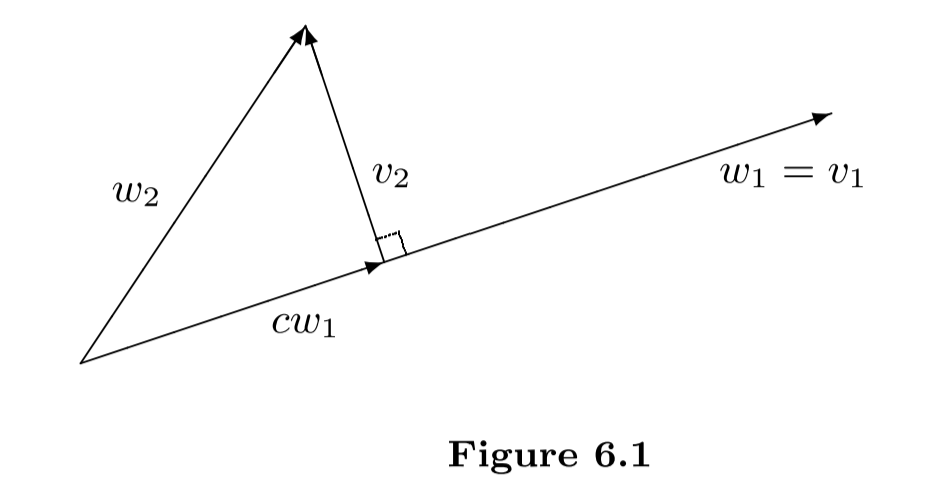
\includegraphics[width=10cm]{images/figure-6-1.png}

To find \(c\), we need only solve the following equation:
\[
    0 = \LG v_2, w_1 \RG = \LG w_2 - cw_1, w_1 \RG = \LG w_2, w_1 \RG - c \LG w_1, w_1 \RG.
\]
So
\[
    c = \frac{\LG w_1, w_2 \RG}{ \norm{w_1}^2 }
\]
Thus
\[
    v_2 = w_2 - c w_1 = w_2 - \frac{\LG w_1, w_2 \RG}{ \norm{w_1}^2 } w_1.
\]
The next theorem shows us that this process can be \emph{extended} to any \emph{finite} linearly independent subset.
\end{remark}

\begin{theorem} [Gram-Schmidt process] \label{thm 6.4}
Let \(\V\) be an inner product space and \(S = \{ w_1, w_2, ..., w_n \}\) be a \LID{} susbet of \(\V\).
Define \(S' = \{ v_1, v_2, ..., v_n \}\), where \(v_1 = w_1\) and
\[
    v_k = \RED{w_k} - \sum_{\BLUE{j = 1}}^{k - 1} \frac{\LG \RED{w_k}, \BLUE{v_j} \RG}{\norm{\BLUE{v_j}}^2} \BLUE{v_j} \quad \text{ for } 2 \le k \le n \quad \quad \MAROON{(1)}
\]
Then \(S'\) is an orthogonal set of nonzero vectors such that \(\spann(S') = \spann(S)\).
\end{theorem}

\begin{note}
The intuition is, to get \(v_k\), we need to subtract off any part of \(w_k\) ``that is \emph{not} orthogonal to the new vectors \(v_1, ..., v_{k - 1}\) we have found'', and this part is equal to the summation in \MAROON{(1)};
hence \(v_k\) will be orthogonal to all the previously found \(v_1, ..., v_k\).
\end{note}

\begin{proof}
The proof is by mathematical induction on \(n\), the \emph{number of vectors in} \(S\).
For \(k = 1, 2, ..., n\), let \(S_k = \{ w_1, w_2, ..., w_k \}\).
If \(n = 1\), then the theorem is proved by taking \(S_1' = S_1\); i.e., \(w_1 = v_1 \ne \OV\).
Assume then that the set \(S'_{k - 1} = \{ v_1, v_2, ..., v_{k-1} \}\) \emph{with the desired properties has been constructed}(i.e. \textbf{induction hypothesis}) by the repeated use of \MAROON{(1)}.
We show that the set \(S'_k = \{ v_1, v_2, ..., v_{k - 1}, v_k \}\) also has the desired properties, where \(v_k\) is obtained from \(S'_{k - 1}\) by \MAROON{(1)}.
If \(v_k = \OV\), then \MAROON{(1)} implies that \(w_k \in \spann(S'_{k - 1})\), which (by induction hypothesis) is equal to \(\spann(S_{k-1})\), which contradicts the assumption that \(S_k\) is \LID{}, hence \(v_k\) must be nonzero vector.

Now for \(1 \le i \le k- 1\), it follows from \MAROON{(1)} that
\begin{align*}
    \LG v_k, v_i \RG & = \LG w_k - \sum_{j = 1}^{k - 1} \frac{\LG w_k, v_j \RG}{\norm{v_j}^2} v_j, v_i \RG & \text{by \MAROON{(1)}} \\
        & = \LG w_k, v_i \RG - \sum_{j = 1}^{k - 1} \frac{\LG w_k, v_j \RG}{\norm{v_j}^2} \LG v_j, v_i \RG & \text{by \DEF{6.1}(a)(b)} \\
        & = \LG w_k, v_i \RG - \frac{\LG w_k, v_i \RG}{\norm{v_i}^2} \LG v_i, v_i \RG & \text{since \(S'\) is orthogonal by induction hypo} \\
        & = \LG w_k v_i \RG - \frac{\LG w_k, v_i \RG}{\norm{v_i}^2} \norm{v_i}^2 & \text{by \DEF{6.3}} \\
        & = \LG w_k v_i \RG - \LG w_k, v_i \RG = 0 & \text{of course}
\end{align*}
Hence \(v_k\) is orthogonal to \(v_1, ..., v_{k - 1}\).
With induction hypothesis that \(S'_{k - 1} = \{ v_1, ..., v_{k - 1} \}\) is orthogonal, we have that \(S'_k\) is an orthogonal set of nonzero vectors.

Now by induction hypothesis, \(\{ v_1, ..., v_{k - 1} \} = S'_{k - 1} = S_{k - 1} \subseteq S_k\).
And by \MAROON{(1)}, since each term of the right hand side is in \(S_k\), we have \(v_k\), the left hand side, in \(S_k\);
hence \(S'_{k - 1} \cup \{ v_k \} \subseteq S_k\); that is, \(S'_k \subseteq S_k\).
But (since \(S'_k\) is orthogonal and has nonzero vectors,) by \CORO{6.3.2} \(S'_k\) is \LID{}, so \(\dim(\spann(S'_k)) = k\).
But since \(S_k\) is also \LID{}, \(\dim(\spann(S_k)) = k\).
Therefore (by \THM{1.11}) \(\spann(S'_k) = \spann(S_k)\).
This closes the induction.
\end{proof}

\begin{remark} \label{remark 6.2.3}
The construction of \(\{ v_1, v_2, ..., v_n \}\) by the use of \THM{6.4} is called the \textbf{Gram-Schmidt process}.
And note that whether a set can be called orthogonal or orthonormal \textbf{depends on the inner product you choose}.
For example, the standard ordered basis for \(F^n\) is an orthonormal basis with respect to \emph{standard} inner product.
But it is not an orthonormal basis with respect to an inner product, say, \(\InnerOp' = 2 \InnerOp\), since the norm of each \(e_i\) is \(\norm{e_i}' = \sqrt{\LG e_i, e_i \RG'} = \sqrt{2 \LG e_i, e_i \RG } = \sqrt{2 \cdot 1} = \sqrt{2}\), which is not equal to \(1\).
\end{remark}

\begin{example} \label{example 6.2.4}
In \(\SET{R}^4\), let \(w_1 = (1, 0, 1, 0), w_2 = (1, 1, 1, 1)\), and \(w_3 = (0, 1, 2, 1)\).
Then \(\{ w_1, w_2, w_3 \}\) is \LID{}.
We use the Gram-Schmidt process to compute the orthogonal vectors \(v_1, v_2\), and \(v_3\), and then we normalize these vectors to obtain an orthonormal set.

Take \(v_1 = w_1 = (1, 0, 1, 0)\).
Then
\begin{align*}
    v_{\RED{2}} & = w_{\RED{2}} - \sum_{j = 1}^{\RED{2} - 1} \frac{\LG w_{\RED{2}}, v_j \RG}{\norm{v_j}^2} v_j & \text{by \THM{6.4}} \\
        & = w_2 - \frac{\LG w_2, v_1 \RG}{\norm{v_1}^2} v_1 \\
        & = (1, 1, 1, 1) - \frac{2}{2}(1, 0, 1, 0) = (0, 1, 0, 1)
\end{align*}
And
\begin{align*}
    v_{\RED{3}} & = w_{\RED{3}} - \sum_{j = 1}^{\RED{3} - 1} \frac{\LG w_{\RED{3}}, v_j \RG}{\norm{v_j}^2} v_j & \text{by \THM{6.4}} \\
        & = w_3 - \frac{\LG w_3, v_1 \RG}{\norm{v_1}^2} v_1 - \frac{\LG w_3, v_2 \RG}{\norm{v_2}^2} v_2 \\
        & = (0, 1, 2, 1) - \frac{2}{2} (1, 0, 1, 0) - \frac{2}{2} (0, 1, 0, 1) = (-1, 0, 1, 0).
\end{align*}
These vectors can be normalized to obtain the ortho\emph{normal} basis \(\{ u_1, u_2, u_3 \}\), where
\begin{align*}
    u_1 & = \frac{1}{\norm{v_1}} v_1 = \frac{1}{\sqrt{2}}(1, 0, 1, 0), \\
    u_2 & = \frac{1}{\norm{v_2}} v_2 = \frac{1}{\sqrt{2}}(0, 1, 0, 1), \\
    u_3 & = \frac{1}{\norm{v_3}} v_3 = \frac{1}{\sqrt{2}}(-1, 0, 1, 0).
\end{align*}
\end{example}

\begin{example} \label{example 6.2.5}
Let \(\V = \POLYRINF\) with the inner product
\[
    \LG f(x), g(x) \RG = \int_{-1}^{1} f(t)g(t) dt,
\]
and consider the subspace \(\POLYRR\) with the \emph{standard} ordered basis \(\beta = \{ w_1, w_2, w_3 \} = \{ 1, x, x^2 \}\).
(Note that, the point is, \(\beta\) may not be an \emph{orthogonal} basis with respect to \emph{this} inner product.)
We use the Gram Schmidt process to replace \(\beta\) by an orthogonal basis \(\{v_1, v_2, v_3 \}\) for \(\POLYRR\), \emph{with respect to} this inner product, and then use this orthogonal basis to obtain an orthonormal basis for \(\POLYRR\).

So by the process, take \(v_1 = 1\).
Then \(\norm{v_1}^2 = \LG 1, 1 \RG = \int_{-1}^1 1 \cdot 1 dt = 2\), and \(\LG x, v_1 \RG = \int_{-1}^1 t \cdot 1 dt = 0\).
Thus
\begin{align*}
    v_2 & = x - \frac{\LG x, v_1 \RG}{\norm{v_1}^2} & \text{by \THM{6.4}} \\
        & = x - \frac{0}{2} = x.
\end{align*}
Furthermore,
\[
    \LG x^2, v_1 \RG = \int_{-1}^1 t^2 \cdot 1 dt = \frac{2}{3} \quad \text{ and } \quad \LG x^2, v_2 \RG = \int_{-1}^1 t^2 \cdot t dt = 0.
\]
Therefore
\begin{align*}
    v_3 & = x^2 - \frac{\LG x^2, v_1 \RG}{\norm{v_1}^2} v_1 - \frac{\LG x^2, v_2 \RG}{\norm{v_2}^2} v_2 & \text{by \THM{6.4}} \\
        & = x^2 - \frac{1}{3} \cdot 1 - 0 \cdot x \\
        & = x^2 - \frac{1}{3}.
\end{align*}
We conclude that \(\{ 1, x, x^2 - \frac{1}{3} \}\) is an orthogonal basis for \(\POLYRR\) with respect to this inner product.

To obtain an ortho\emph{normal} basis, we normalize \(v_1, v_2\), and \(v_3\) to obtain
\begin{align*}
    u_1 & = \frac{1}{\sqrt{\int_{-1}^1 1^2 dt}} \cdot 1 = \frac{1}{\sqrt{2}}, \\
    u_2 & = \frac{1}{\sqrt{\int_{-1}^1 t^2 dt}} \cdot x = \sqrt{\frac{3}{2}} x, \\
    u_3 & = \frac{1}{\norm{v_3}} \cdot v_3 = \sqrt{\frac{5}{8}}(3x^2 - 1).
\end{align*}
Thus \(\{ u_1, u_2, u_3 \}\) is the desired orthonormal basis for \(\POLYRR\).
\end{example}

\begin{remark} \label{remark 6.2.4}
Continuing to apply the Gram-Schmidt orthogonalization process to the basis \(\{ 1, x, x^2, ... \}\) for \(\POLYRINF\), we obtain an ortho\emph{\textbf{\RED{gonal}}} basis \(\{ v_1, v_2, v_3, ... \}\).
Note that we do \emph{not} normalize them, so in particular, from \EXAMPLE{6.2.5},
\[
    \{ v_1, v_2, v_3 \} = \left\{ 1, x, x^2 - \frac{1}{3} \right\}.
\]
For each \(n\), the polynomial
\[
    \frac{1}{v_k(1)} v_k
\]
is called the \(k\)th \textbf{\href{https://www.wikiwand.com/en/Legendre_polynomials\#/Orthogonality_and_completeness}{Legendre polynomial}}.

(I don't know why we also need to multiply this additional scalar \(\frac{1}{v_k(1)}\).
In particular, why it must be true that \(v_k(1) \ne 0\) for all positive integer \(k\)?)

Then first three Legendre polynomials are
\begin{align*}
    \frac{1}{v_1(1)} v_1 & = \frac{1}{1} 1 = 1 \\
    \frac{1}{v_2(1)} v_2 & = \frac{1}{1} x = x \\
    \frac{1}{v_3(1)} v_3 & = \frac{1}{1 - \frac{1}{3}} \left( x^2 - \frac{1}{3} \right) = \frac{1}{2}(3x^2 - 1).
\end{align*}
The set of Legendre polynomials is also an orthogonal basis for \(\POLYRINF\).
\end{remark}

The following result gives us a simple method of representing a vector as a linear combination of the vectors in an ortho\emph{normal} basis.

\begin{theorem} \label{thm 6.5}
Let \(\V\) be a nonzero \emph{finite}-dimensional inner product space.
Then \(\V\) \textbf{has} an orthonormal basis \(\beta\).
Furthermore. if \(\beta = \{ v_1, v_2, ..., v_n \}\) and \(x \in \V\), then
\[
    x = \sum_{i = 1}^n \LG x, v_i \RG v_i.
\]
\end{theorem}

\begin{note}
要證明無限維度內積空間有標準正交基底也需要選擇公里或\ Zorn's Lemma.
\end{note}

\begin{proof}
Let \(\beta_0\) be an ordered basis for \(\V\).
Apply \THM{6.4} to obtain an orthogonal \emph{set} \(\beta'\) of nonzero vectors with \(\spann(\beta') = \spann(\beta_0) = \V\).
By normalizing each vector in \(\beta'\), we obtain an orthonormal \emph{set} \(\beta\) that generates \(\V\).
By \CORO{6.3.2}, \(\beta\) is \LID{}; therefore \(\beta\) is an orthonormal \emph{basis} for \(\V\).
The remainder of the theorem follows from \CORO{6.3.1}.
\end{proof}

\begin{example} \label{example 6.2.6}
We use \THM{6.5} to represent the polynomial \(f(x) = 1 + 2x + 3x^2\) as a linear combination of the vectors in the \emph{orthonormal} basis \(\{ u_1, u_2, u_3 \}\) for \(\POLYRR\) obtained in \EXAMPLE{6.2.5}.
Observe that
\[
    \LG f(x), u_1 \RG = \int_{-1}^{1} \frac{1}{\sqrt{2}} (1+2 t+3 t^2) \cdot 1 dt = 2 \sqrt{2}
\]
\[
    \LG f(x), u_2 \RG = \int_{-1}^{1} \sqrt{\frac{3}{2}} (1+2 t+3 t^2) \cdot t dt = \frac{2 \sqrt{6}}{3}
\]
and
\[
    \LG f(x), u_3 \RG = \int_{-1}^{1} \sqrt{\frac{5}{8}} (1 + 2t + 3t^2) (3 t^2 - 1) d t = \frac{2 \sqrt{10}}{5}.
\]
So by \THM{6.5}, \(f(x) = \LG f(x), u_1 \RG u_1 + \LG f(x), u_2 \RG u_2 + \LG f(x), u_3 \RG u_3 = 2 \sqrt{2} u_1 + \frac{2 \sqrt{6}}{3} u_2 + \frac{2 \sqrt{10}}{5} u_3\).
\end{example}

\THM{6.5} gives us a simple method for computing the entries of the \textbf{matrix representation} of a linear operator \textbf{with respect to an orthonormal basis}.

\begin{corollary} \label{corollary 6.5.1}
Let \(\V\) be a \emph{finite}-dimensional inner product space with an \emph{orthonormal} basis \(\beta = \{ v_1, v_2, ..., v_n \}\).
Let \(\T\) be a linear operator on \(\V\), and let \(A = [\T]_{\beta}\).
Then for any \(i\) and \(j\), \(A_{ij} = \LG \T(v_j), v_i \RG\).
(Notice the order of \(i\) and \(j\) in the equation.)
\end{corollary}

\begin{proof}
In particular from \THM{6.5}, we have
\[
    \T(v_j) = \sum_{i = 1}^n \LG \T(v_j), v_i \RG v_i.
\]
Hence by definition of matrix representation, \(A_{ij} = \LG \T(v_j), v_i \RG\).
\end{proof}

\begin{remark} \label{remark 6.2.5}
The scalars \(\LG x, v_i \RG\) given in \THM{6.5} have been studied \emph{extensively} for special inner product spaces. 
Although the vectors \(v_1, v_2, ..., v_n\) were chosen from an orthonormal basis, we introduce a terminology associated
with orthonormal sets \(\beta\) in more general inner product spaces.
\end{remark}

\begin{definition} \label{def 6.6}
Let \(\beta\) be an orthonormal subset (possibly infinite) of an inner product space \(\V\), and let \(x \in \V\).
We define the \textbf{Fourier coefficient\RED{s}} of \(x\) relative to \(\beta\) to be the scalars \(\LG x, y \RG\), where \(y \in \beta\).
\end{definition}

\begin{remark} \label{remark 6.2.6}
In the first half of the 19th century, the French mathematician Jean Baptiste Fourier was associated with the study of the \emph{scalars} (for any integer \(n\))
\[
    \int_0^{2\pi} f(t) \sin nt dt \quad \text{ and } \quad \int_0^{2\pi} f(t) \cos nt dt
\]
or in the complex case,
\[
    c_n = \frac{1}{2\pi} f(t) e^{-\iu n t} dt.
\]
for a function \(f\).
In the context of \EXAMPLE{6.1.9}, we see that \(c_n = \LG f, f_n \RG\), where \(f_n(t) = e^{\iu nt}\); that is, \(c_n\) is the nth \emph{Fourier coefficient} for a continuous function \(f \in \textsf{H}\) relative to \(S\).
The coefficients \(c_n\) are the ``classical'' Fourier coefficients of a function, and the literature concerning their behavior is extensive.
We learn more about Fourier coefficients in the remainder of this chapter.
\end{remark}

\begin{example} \label{example 6.2.7}
Let \(S = \{ e^{\iu n t} : n \text{ is an integer} \}\).
In \EXAMPLE{6.1.9}, \(S\) was shown to be an orthonormal set in \(\textsf{H}\).
We compute the Fourier coefficients of \(f(t) = t\) relative to \(S\).
Using \emph{integration by parts}, we have, for \(n \ne 0\),
\[
    \LG f, f_n \RG = \frac{1}{2\pi} \int t \conjugatet{e^{\iu n t}} dt = \int \frac{1}{2\pi} t e^{-\iu n t} dt = \frac{-1}{\iu n}, \quad \MAROON{(1)}
\]
and, for \(n = 0\),
\[
    \LG f, f_n \RG = \LG f, e^0 \RG = \LG f, 1 \RG = \int \frac{1}{2\pi} t \cdot 1 dt = \pi. \quad \MAROON{(2)}
\]
As a result of these computations, and using \EXEC{6.2.16}, we obtain an \emph{upper bound} for the sum of a special \emph{infinite series}, \(\sum_{i = 1}^{\infty} \frac{1}{n^2}\), as follows:
(Note that since \(S\) is orthonormal, in particular \(S_k = \{ e^{\iu n t} : -k \le n \le k \}\) is orthonormal.)
\begin{align*}
    \norm{f}^2 & \ge \sum_{n = -k}^k \abs{ \LG f, f_n \RG }^2 & \text{by \EXEC{6.2.16} with aforementioned \(S_k\)} \\
        & = \sum_{n = -k}^{-1} \abs{ \LG f, f_n \RG }^2 + \abs{ \LG f, 1 \RG }^2 + \sum_{n = 1}^k \abs{f, f_n}^2 \\
        & = \sum_{n = -k}^{-1} \frac{1}{n^2} + \pi^2 + \sum_{n = 1}^k \frac{1}{n^2} & \text{by using \MAROON{(1)(2)}, but taking square} \\
        & = 2 \sum_{n = 1}^k \frac{1}{n^2} + \pi^2 & \text{of course}
\end{align*}
for every \(k\).

Now, using the fact that \(\norm{f}^2 = \frac{4}{3}\pi^2\), we obtain
\[
    \frac{4}{3}\pi^2 \ge 2 \sum_{n = 1}^k \frac{1}{n^2} + \pi^2,
\]
or
\[
    \frac{\pi^2}{6} \ge \sum_{n = 1}^k \frac{1}{n^2}.
\]
Because this inequality holds \emph{for all} \(k\), we may let \(k \to \infty\) to obtain
\[
    \frac{\pi^2}{6} \ge \sum_{n = 1}^{\infty} \frac{1}{n^2}.
\]
Additional results may be produced by replacing \(f\) by other functions.
\end{example}

\begin{note}
(My professor said) The inequality we have shown is in fact an equality, but the proof need some technique in Analysis courses.
\end{note}

We are now ready to proceed with the concept of an \emph{orthogonal complement}.

\begin{definition} \label{def 6.7}
Let \(S\) be a nonempty subset of an inner product space \(\V\).
We define \(S^{\perp}\) (read ``\(S\) perp'') to be the set of all vectors in \(\V\) that are \emph{orthogonal} to every vector in \(S\);
that is, \(S^{\perp} = \{ x \in \V: \LG x, y \RG = 0 \text{ for all } y \in S\}\).
The set \(S^{\perp}\) is called the \textbf{orthogonal complement} of \(S\).

It is easily seen that \(S^{\perp}\) is a subspace of \(\V\) for any subset \(S\) of \(\V\). (See \EXEC{6.2.1}(c).)

And in particular, if \(S\) itself is also a subspace, then \(S \cap S^{\perp} = \{ \OV \}\).
(Otherwise if \(v \in S\) and \(v \in S^{\perp}\) where \(v \ne \OV\), the we have \(\LG \BLUE{v}, \RED{v} \RG = 0\) where \(\BLUE{v} \in S^{\perp}\) and \(\RED{v} \in S\), but this contradicts \DEF{6.1}(d).)
\end{definition}

\begin{example} \label{example 6.2.8}
The reader should verify that \(\{ \OV \}^{\perp} = \V\) and \(\V^{\perp} = \{ \OV \}\) for any inner product space \(\V\).
\end{example}

\begin{example} \label{example 6.2.9}
If \(\V = \SET{R}^3\) and \(S = \{ e_3 \}\), then \(S^{\perp}\) equals the \(xy\)-plane (see \EXEC{6.2.5}).
\end{example}

\EXEC{6.2.18} provides an interesting example of an orthogonal complement in an \emph{infinite}-dimensional inner product space. 
\begin{remark} \label{remark 6.2.7}
Consider the problem in \(\SET{R}^3\) of finding the \emph{distance} from a point \(P\) to a plane \(\W\).
(See Figure 6.2.)

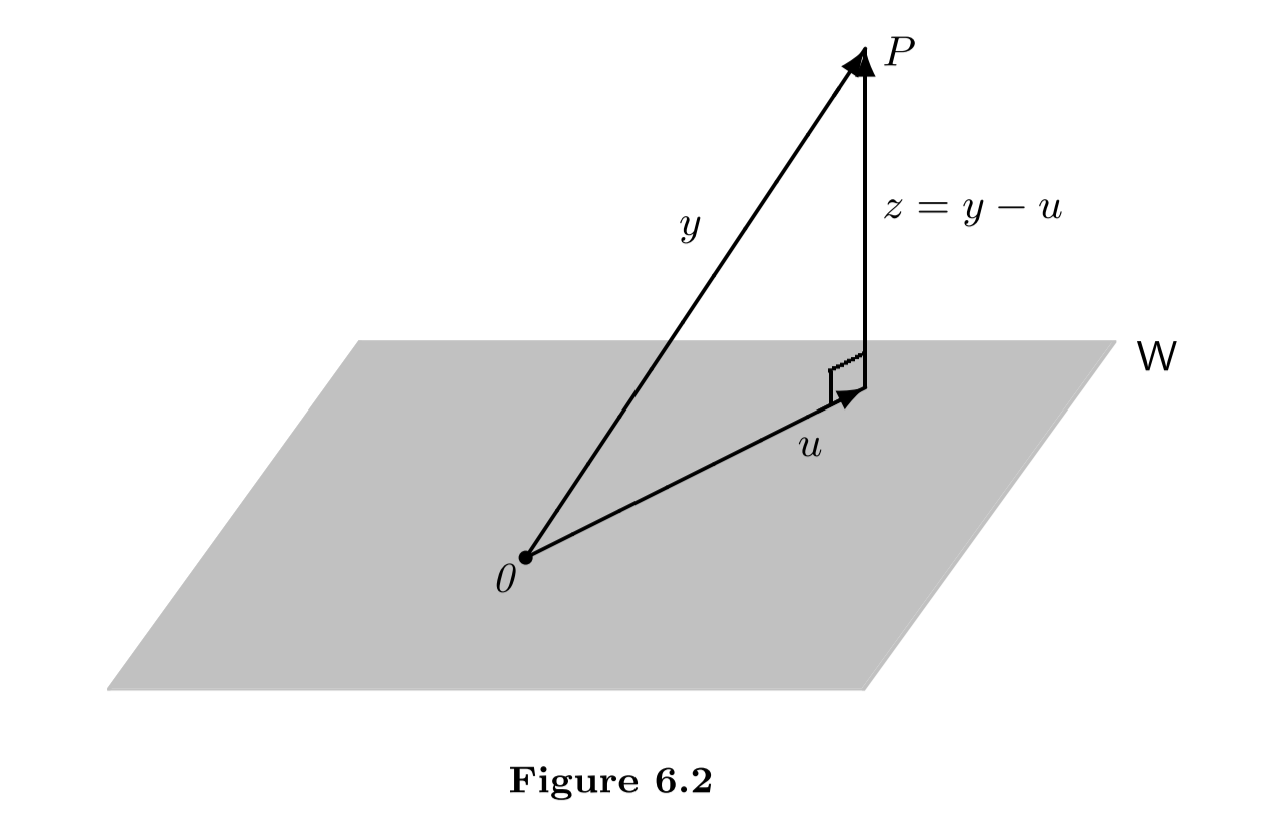
\includegraphics[width=12cm]{images/figure-6-2.png}

(This is high school algebra, but) Problems of this type arise in many settings.
If we let \(y\) be the vector determined by \(0\) and \(P\).
We may restate the problem as follows:
Determine the vector \(u\) in \(\W\) that is ``\textbf{closest}'' to \(y\).
The desired distance is clearly given by \(\norm{y - u}\).
\emph{Notice} from the figure that the vector \(z = y - u\) is \emph{orthogonal} to \textbf{every vector} in \(\W\), and so \(z \in \W^{\perp}\).

The next result presents a practical method of finding \(u\) in the case that \(\W\) is a \emph{finite}-dimensional \emph{subspace} of an inner product space.
\end{remark}

\begin{theorem} \label{thm 6.6}
Let \(\W\) be a \emph{finite}-dimensional subspace of an inner product space \(\V\), and let \(y \in \V\).
Then \emph{there exist} \textbf{unique} vector \(u \in \W\) and \textbf{unique} vector \(z \in \W^{\perp}\), such that \(y = u + z\).
Furthermore, if \(\{ v_1, v_2, ..., v_k \}\) is an orthonormal basis \textbf{for \(\W\)}, then
\[
    u = \sum_{i = 1}^k \LG y, v_i \RG v_i.
\]
\end{theorem}

\begin{note}
\THM{6.6} 就是最廣義的看法:
給定一個子空間 \(\W\),然後給定一個向量\ \(y \in \V\),這個向量\ \(y\) 可以拆成\textbf{唯一的}表示法\ \(u + z\),使得\ \(u \in \W\),\(z \in \W^{\perp}\)。
另外\ \(u\) 就是\ \textbf{\(y\) 在\ \(\W\) 的「投影」},並且可用\ \(\W\) 的\ orthonormal basis 來表示,係數就是\ \(y\) 對每個\ basis vector 的投影量。
如果是\ \(\SET{R}^3\) 的例子就會是\ Figure 6.2。
\end{note}

\begin{proof}
Let \(\{ v_1, v_2, ..., v_k \}\) be an orthonormal basis for \(\W\), let \(u\) be as defined in the preceding equation, and let \(z = y - u\). Clearly \(u \in \W\) and \(y = u + z\).

To show that \(z \in \W^{\perp}\), it suffices to show, by \EXEC{6.2.7}, that \(z\) is orthogonal to each \(v_j\) for \(1 \le j \le k\).
So for any \(j\), we have
\begin{align*}
    \LG z, v_j \RG & = \LG y - u, v_j \RG = \LG y - \sum_{i = 1}^k \LG y, v_i \RG v_i, v_j \RG & \text{of course} \\
        & = \LG y, v_j \RG - \sum_{i = 1}^k \LG y, v_i \RG \LG v_i, v_j \RG & \text{by \DEF{6.1}(a)(b)} \\
        & = \LG y, v_j \RG - \LG y, v_{\RED{j}} \RG \LG v_{\RED{j}}, v_j \RG & \text{since \(v_i\)'s are in particular orthogonal} \\
        & = \LG y, v_j \RG - \LG y, v_{j} \RG \norm{v_j}^2 & \text{by \DEF{6.3}} \\
        & = \LG y, v_j \RG - \LG y, v_{j} \RG \cdot 1 = \LG y, v_j \RG - \LG y, v_{j} \RG & \text{since \(v_i\)'s are ortho\emph{normal}} \\
        & = 0.
\end{align*}
Hence \(z \in \W^{\perp}\), hence the existence part that \(y = u + z\) where \(u \in \W\) and \(z \in \W^{\perp}\) is showed.

Now for the uniqueness part, suppose that \(y = u + z = u' + z'\), where \(u' \in \W\) and \(z' \in \W^{\perp}\).
Then in particular by arranging equation, \(u - u' = z'- z\); but \(u - u' \in \W\) and \(z' - z \in \W^{\perp}\), so the equation implies both \(u - u', z' - z \in \W \cap \W^{\perp}\).
But in \DEF{6.7} we have shown \(\W \cap \W^{\perp} = \{ \OV \}\), hence \(u - u' = z' - z = \OV\), hence \(u = u'\) and \(z = z'\), showing the uniqueness.
\end{proof}

\begin{corollary} \label{corollary 6.6.1}
In the notation of \THM{6.6}, the vector \(u\) is the unique vector in \(\W\) that is ``closest'' to \(y\);
that is, for any \(x \in \W\), \(\norm{y - x} \ge \norm{y - u}\), and this inequality is an equality if and only if \(x = u\).
\end{corollary}

\begin{proof}
As in \THM{6.6}, we have that \(y = u + z\), where \(z \in \W^{\perp}\).
Let \(x \in \W\).
Then \(u - x \in \W\), hence is orthogonal to \(z\). \MAROON{(1)}

So by \EXEC{6.1.10}, we have
\begin{align*}
    \norm{y - x}^2 & = \norm{(u + z) - x}^2 = \norm{(u - x) + z^2} & \text{tricky but of course} \\
        & = \norm{u - x}^2 + \norm{z}^2 & \text{by \MAROON{(1)} and \EXEC{6.1.10}} \\
        & \ge \norm{z}^2 & \text{by \THM{6.2}(b), \(\norm{u - x}^2 \ge 0\)} \\
        & = \norm{y - u}^2, & \text{of course}
\end{align*}
which implies \(\norm{y - x} \ge \norm{y - u}\).

Now suppose that \(\norm{y - x} = \norm{y - u}\).
Then the inequality above becomes an equality, and therefore \(\norm{u - x}^2 + \norm{z}^2 = \norm{z}^2\).
It follows that \(\norm{u - x} = 0\), and hence (by \THM{6.2}(a)) \(x = u\).

For the converse, if \(x = u\), then of course \(y - x = y - u\) hence of course \(\norm{y - x} = \norm{y - u}\).
\end{proof}

\begin{additional definition} \label{adef 6.3}
The vector \(u\) in the corollary is called the \textbf{orthogonal projection} of \(y\) on \(\W\).
We will see the importance of orthogonal projections of vectors in the application to \emph{least squares} in \SEC{6.3}.
\end{additional definition}

\begin{example} \label{example 6.2.10}
Let \(\V = \POLYRRR\) with the inner product
\[
    \LG f(x),g(x) \RG = \int_{-1}^{1} f(t)g(t) dt
\]
for all \(f(x), g(x) \in \V\).
We compute the orthogonal projection of \(f(x) = x^3\) on \(\POLYRR\).
Let it be \(f_1(x)\).

By \EXAMPLE{6.2.5},
\[
    \{ u_1, u_2, u_3 \} = \left\{ \frac{1}{\sqrt{2}}, \sqrt{\frac{3}{2}} x, \sqrt{\frac{5}{8}}(3x^2 - 1) \right\}
\]
is an orthonormal basis for \(\POLYRR\).
By \THM{6.6}, we need to compute \(\LG f(x), u_1 \RG, \LG f(x), u_2 \RG\) and \(\LG f(x), u_3 \RG\).
So we have
\[
    \LG f(x), u_1 \RG = \int_{-1}^{1} t^3 \frac{1}{\sqrt{2}} dt = 0,
    \quad \LG f(x), u_2 \RG = \int_{-1}^{1} t^3 \sqrt{\frac{3}{2}} t dt = \frac{\sqrt{6}}{5}
\]
and
\[
    \LG f(x), u_3 \RG = \int_{-1}^{1} t^{3} \sqrt{\frac{5}{8}} (3 t^2 - 1) dt = 0
\]
Hence
\begin{align*}
    f_{1}(x) & = \LG f(x), u_1 \RG u_1 + \LG f(x), u_2 \RG u_2 + \LG f(x), u_3 \RG u_3 & \text{by \THM{6.6}} \\
        & = 0 u_1 + \frac{\sqrt{6}}{5} u_2 + 0 u_3 \\
        & = \frac{\sqrt{6}}{5} \cdot \sqrt{\frac{3}{2}}x = \frac{3}{5} x
\end{align*}
\end{example}

\begin{remark} \label{remark 6.2.8}
It was shown in \CORO{1.10.2}(corollary to the replacement theorem) that any \LID{} set in a \emph{finite}-dimensional vector space can be \emph{extended} to a basis.
The next theorem provides an interesting analog for an orthonormal subset of a \emph{finite}-dimensional inner product space.
\end{remark}

\begin{theorem} \label{thm 6.7}
Suppose that \(S = \{ v_1, v_2, ..., v_k \}\) is an orthonormal set in an \(n\)-dimensional inner product space \(\V\).
Then
\begin{enumerate}
\item \(S\) can be extended to an \textbf{orthonormal} basis \(\{ v_1, v_2, ..., v_k, v_{k+1}, ..., v_n \}\) for \(\V\).
\item If \(\W = \spann(S)\), then \(S_1 = \{v_{k+1}, v_{k+2}, ..., v_n \}\) is an orthonormal basis for \(\W^{\perp}\) (using the preceding notation).
\item If \(\W\) is any \emph{subspace} of \(\V\), then \(\dim(\V) = \dim(\W) + \dim(\W^{\perp})\).
\end{enumerate}
\end{theorem}

\begin{proof} \ 

\begin{enumerate}
\item By \CORO{1.10.2}, \(S\) can be extended to an \emph{ordered basis} \(S' = \{ v_1, v_2, ..., v_{k}, w_{k+1}, ..., w_n \}\) for \(\V\).
Now apply the Gram-Schmidt process to \(S'\).
By \EXEC{6.2.8}, the first \(k\) vectors resulting from this process \textbf{are still the vectors in \(S\)} , and this new set spans \(\V\).
Normalizing the last \(n - k\) vectors of this set produces an orthonormal set that spans \(\V\).
The result now follows.

\item Because \(S_1\) is a subset of a (orthonormal) basis, it is \LID{}.
And for every vector in \(S_1\), it is orthogonal to every vector in \(S\), hence is orthogonal to every vector in \(\spann(S) = \W\), so by \DEF{6.7} it is in \(\W^{\perp}\), hence \(S_1 \subseteq \W^{\perp}\).

Now we show that it spans \(\W^{\perp}\).
Note that \(\spann(S_1) \subseteq \W^{\perp}\) is automatically true.
And for any \(x \in \V\), since \(\{ v_1, v_2, ..., v_n \}\) is an orthonormal basis, (by \THM{6.5}) we have
\[
    x = \sum_{i = 1}^n \LG x, v_i \RG v_i.
\]
Now if \(x\) is also in \(\W^{\perp}\), then \(\LG x, v_i \RG = 0\) for \(1 \le i \le k\).
Therefore
\[
    x = \sum_{i = k + 1}^n \LG x, v_i \RG v_i \in \spann(S_1).
\]
Hence \(\W^{\perp} \subseteq \spann(S_1)\).
Hence \(\W^{\perp} = \spann(S_1)\).
So \(S_1\) generates \(\W^{\perp}\) and is \LID{}, hence is a basis for \(\W^{\perp}\).

\item Let \(\W\) be a subspace of \(\V\).
It is a \emph{finite}-dimensional inner product space because \(\V\) is, and so it has an orthonormal basis \(\{ u_1, u_2, ..., u_k \}\).
By (a) and (b). we have
\begin{align*}
    & \dim(\V) \\
    & = n = k + (n - k) & \text{of course} \\
    & = \dim(\W) + (n - k) & \text{\(\{ u_1, ..., u_k \}\) is a basis for \(\W\)} \\
    & = \dim(\W) + \dim(\W^{\perp}) & \text{by (a)(b), the extended \(\{ u_{k + 1}, ..., u_{n} \}\) is a basis for \(\W^{\perp}\)}
\end{align*}
\end{enumerate}
\end{proof}

\begin{example} \label{example 6.2.11}
Let \(\W = \spann(\{ e_1, e_2 \})\) in \(F^3\).
Then \(x = (a, b, c) \in \W^{\perp}\) if and only if \(0 = \LG x, e_1 \RG = a\) and \(0 = \LG x , e_2 \RG = b\).
So \(x = (0, 0, c)\), and therefore \(\W^{\perp} = \spann(\{ e_3 \})\).
One can deduce the same result by noting that \(e_3 \in \W^{\perp}\) and, from \THM{6.7}(c), that \(\dim(\W^{\perp}) = \dim(V) - \dim(W) = 3 - 2 = 1\).
\end{example}

\exercisesection

\begin{exercise} \label{exercise 6.2.1}
Label the following statements as true or false.
\begin{enumerate}
\item The Gram-Schmidt orthogonalization process produces an orthonormal set from an arbitrary \emph{\LID{}} set.
\item Every nonzero finite-dimensional inner product space has an orthonormal basis.
\item The orthogonal complement of any set is a subspace.
\item If \(\{ v_1, v_2, ..., v_n \}\) is a basis for an inner product space \(\V\), then for any \(x \in \V\) the scalars \(\LG x, v_i \RG\) are the Fourier coefficients of \(x\).
\item An orthonormal basis must be an ordered basis.
\item Every orthogonal set is linearly independent.
\item Every orthonormal set is linearly independent.
\end{enumerate}
process 那提很尷尬;gen 出來的嚴格來說是 orthogonal,但是把 process 多一步做 normalize 也可以吧
Fourier coefficients 那個,basis 要 orthonormal ==
\end{exercise}

\begin{proof}
\end{proof}

\begin{exercise} \label{exercise 6.2.2}
In each part, apply the Gram-Schmidt process to the given subset \(S\) of the inner product space \(\V\) to obtain an orthogonal basis for \(\spann(S)\).
Then normalize the vectors in this basis to obtain an orthonormal basis \(\beta\) for \(\spann(S)\), and compute the Fourier coefficients of the given vector relative to \(\beta\).
Finally, use \THM{6.5} to verify your result.

\begin{enumerate}
\item \(\V = \SET{R}^3, S = \{ (1, 0, 1), (0, 1, 1), (1, 3, 3) \}\), and \(x = (1, 1, 2)\)
\item \(\V = \SET{R}^3, S = \{ (1, 1, 1), (0, 1, 1), (0, 0, 1) \}\), and \(x = (1, 0, 1)\)
\item \(\V = \POLYRR\) with the inner product \(\LG f(x), g(x) \RG = \int_0^1 f(t) g(t) dt, S = \{1, x, x^2 \}\), and \(h(x) = 1 + x\)
\item \(\V = \spann(S)\), where \(S = \{(1, \iu, 0), (1 - \iu, 2, 4\iu) \}\), and \(x = (3 + \iu, 4\iu, -4)\)
\item \(\V = \SET{R}^4, S = \{ (2, -1, -2, 4), (-2, 1, -5, 5), (-1, 3, 7, 11) \}\), and \(x = (-11, 8, -4, 18)\)
\item \(\V = \SET{R}^4, S = \{ (1, -2, -1, 3), (3, 6, 3, -1), (1, 4, 2, 8) \}\), and \(x = (-1, 2, 1, 1)\)
\item \(\V = M_{2 \X 2}(\SET{R}),
    S = \left\{
        \begin{pmatrix}3 & 5 \\ -1 & 1\end{pmatrix},
        \begin{pmatrix}-1 & 9 \\ 5 & -1\end{pmatrix},
        \begin{pmatrix}7 & -17 \\ 2 & -6\end{pmatrix}\right
    \}\),
    and \(A = \begin{pmatrix}-1 & 27 \\ -4 & 8\end{pmatrix}\)
\item \(\V = M_{2 \X 2}(\SET{R}),
    S = \left\{
        \begin{pmatrix}2 & 2 \\ 2 & 1\end{pmatrix},
        \begin{pmatrix}11 & 4 \\ 2 & 5\end{pmatrix},
        \begin{pmatrix}4 & -12 \\ 3 & -16\end{pmatrix}
    \right\}\),
    and \(A = \begin{pmatrix}8 & 6 \\ 25 & -13\end{pmatrix}\)
\item \(\V = \spann(S)\) with the inner product \(\LG f, g \RG = \int_0^{\pi} f(t)g(t) dt, S = \{\sin t, \cos t, 1, t\}\), and \(h(t) = 2t + 1\)
\item \(\V = \SET{C}^4,
    S = \{ (1, i, 2 - \iu, -1), (2 + 3\iu, 3\iu, 1 - \iu, 2\iu), (-1 + 7\iu, 6 + 10\iu, 11 - 4\iu, 3 + 4\iu)\}\),
    and \(x = (-2 + 7\iu, 6 + 9\iu, 9 - 3\iu, 4 + 4\iu)\)
\item \(\V = \SET{C}^4, S = \{(-4, 3 - 2\iu, \iu, 1 - 4\iu), (-1 - 5\iu, 5 - 4\iu, -3 + 5\iu, 7 - 2\iu), (-27 - \iu, -7 - 6\iu, -15 + 25\iu, -7 - 6\iu)\}\), and \(x = (-13 - 7\iu, -12 + 3\iu, -39 - 11\iu, -26 + 5\iu)\)
\item \(\V = M_{2 \X 2}(\SET{C})\),
\[
    S = \left\{
        \begin{pmatrix} 1 - \iu & -2 - 3\iu \\ 2 + 2\iu & 4 + \iu \end{pmatrix},
        \begin{pmatrix} 8\iu & 4 \\ -3 - 3\iu & -4 + 4\iu \end{pmatrix},
        \begin{pmatrix} -25 - 38\iu & -2 - 13\iu \\ 12 - 78\iu & -7 + 24\iu \end{pmatrix}
    \right\},
\]
and \(A=\begin{pmatrix} -2 + 8\iu & -13 + \iu \\ 10 - 10\iu & 9 - 9\iu \end{pmatrix}\)
\item \(\V = M_{2 \X 2}(\SET{C})\),
\[
    S = \left\{
        \begin{pmatrix} -1 + \iu & -\iu \\ 2 - \iu & 1 + 3\iu\end{pmatrix},
        \begin{pmatrix} -1 - 7\iu & -9 - 8\iu \\ 1 + 10\iu & -6 - 2\iu\end{pmatrix},
        \begin{pmatrix} -11 - 132\iu & -34 -31\iu \\ 7 - 126\iu & -71 - 5\iu \end{pmatrix}
    \right\},
\]
and \(A=\begin{pmatrix} -7 + 5\iu & 3 + 18\iu \\ 9 - 6\iu & -3 + 7\iu \end{pmatrix}\)
\end{enumerate}
\end{exercise}

\begin{proof}
手寫吧... 跳過
\end{proof}

\begin{exercise} \label{exercise 6.2.3}
In \(\SET{R}^2\), let
\[
    \beta = \left\{
        \left( \frac{1}{\sqrt{2}}, \frac{1}{\sqrt{2}} \right), \left( \frac{1}{\sqrt{2}}, \frac{-1}{\sqrt{2}} \right)
    \right\}
\]
Find the Fourier coefficients of \((3, 4)\) relative to \(\beta\).
\end{exercise}

\begin{proof}
\end{proof}

\begin{exercise} \label{exercise 6.2.4}
Let \(S = \{ (1, 0, \iu), (1, 2, 1) \}\) in \(\SET{C}^3\). Compute \(S^{\perp}\).
\end{exercise}

\begin{proof}
\end{proof}

\begin{exercise} \label{exercise 6.2.5}
Let \(S_0 = \{ x_0 \}\), where \(x_0\) is a nonzero vector in \(\SET{R}^3\).
Describe \(S_0^{\perp}\) geometrically.
Now suppose that \(S = \{ x_1, x_2 \}\) is a \LID{} subset of \(\SET{R}^3\).
Describe \(S^{\perp}\) geometrically.
\end{exercise}

\begin{proof}
\end{proof}

\begin{exercise} \label{exercise 6.2.6}
Let \(\V\) be an inner product space, and let \(\W\) be a \emph{finite}-dimensional subspace of \(\V\).
If \(x \notin \W\), prove that there \emph{exists} \(y \in \V\) such that \(y \in W^{\perp}\), but \(\LG x, y \RG \ne 0\).
Hint: Use \THM{6.6}.
\end{exercise}

\begin{proof}
\end{proof}

\begin{exercise} \label{exercise 6.2.7}
Let \(\beta\) be a basis for a subspace \(\W\) of an inner product space \(\V\), and let \(z \in \V\).
Prove that \(z \in \W^{\perp}\) if and only if \(\LG z, v \RG = 0\) for every \(v \in \beta\).
\end{exercise}

\begin{note}
又一題,只要檢查 basis 行為就可決定整體行為的。
\end{note}

\begin{proof}
\end{proof}

\begin{exercise} \label{exercise 6.2.8}
Prove that if \(\{ w_1, w_2, ..., w_n \}\) is an \emph{orthogonal} set of nonzero vectors, then the vectors \(v_1, v_2, ..., v_n\) derived from the Gram-Schmidt process \emph{satisfy} \(v_i = w_i\) for \(i = 1, 2, ..., n\).
Hint: Use mathematical induction.
\end{exercise}

\begin{proof}
\end{proof}

\begin{exercise} \label{exercise 6.2.9}
Let \(\W = \spann(\{ ( \iu, 0, 1) \})\) in \(\SET{C}^3\).
Find orthonormal bases for \(\W\) and \(\W^{\perp}\).
\end{exercise}

\begin{proof}
\end{proof}

\begin{exercise} \label{exercise 6.2.10}
Let \(\W\) be a \emph{finite}-dimensional subspace of an inner product space \(\V\).
Prove that \(\V = \W \oplus \W^{\perp}\).
Using the \ADEF{2.2}, prove that there exists a projection \(\T\) on \(\W\) along \(\W^{\perp}\) that satisfies \(\NULLT = \W^{\perp}\).
In addition, prove that \(\norm{\T(x)} \le \norm{x}\) for all \(x \in \V\).
Hint: Use \THM{6.6} and \EXEC{6.1.10}.
\end{exercise}

\begin{proof}
這感覺用 1.6 3x 題 dim v = dim w + dim w perp 可以吧?
\end{proof}

\begin{exercise} \label{exercise 6.2.11}
Let \(A\) be an \(n \X n\) matrix with \emph{complex} entries.
Prove that \(A A^* = I\) if and only if the \emph{rows} of \(A\) form an \emph{orthonormal} basis for \(\SET{C}^n\).
\end{exercise}

\begin{proof}
\end{proof}

\begin{exercise} \label{exercise 6.2.12}
Prove that for any matrix \(A \in M_{m \X n}(F)\), \((\RANGE(\LMTRAN_{A^*}))^{\perp} = \NULL(\LMTRAN_A)\).
\end{exercise}

\begin{note}
幹,怕
A 的零空間會跟 A 的共軛轉置矩陣的 range 的正交補集一樣
\end{note}

\begin{proof}
\end{proof}

\begin{exercise} \label{exercise 6.2.13}
Let \(\V\) be an inner product space, \(S\) and \(S_0\) be \emph{subsets} of \(\V\), and \(\W\) be a finite-dimensional \emph{subspace} of \(\V\).
Prove the following results.
\begin{enumerate}
\item \(S_0 \subseteq S\) implies that \(S^{\perp} \subseteq S_0^{\perp}\).
\item \(S \subseteq (S^{\perp})^{\perp}\); so \(\spann(S) \subseteq (S^{\perp})^{\perp}\).
\item \(\W = (\W^{\perp})^{\perp}\). Hint: Use \EXEC{6.2.6}.
\item \(\V = \W \oplus \W^{\perp}\). (See the exercises of \SEC{1.3}.)
\end{enumerate}
\end{exercise}

\begin{proof}
(d) 在銃殺小? 第十題不就有了?
\end{proof}

\begin{exercise} \label{exercise 6.2.14}
Let \(\W_1\) and \(\W_2\) be subspaces of a \emph{finite}-dimensional inner product space.
Prove that \((\W_1 + \W_2)^{\perp} = \W_1^{\perp} \cap \W_2^{\perp}\) and \((\W_1 \cap \W_2)^{\perp} = \W_1^{\perp} + \W_2^{\perp}\).
Hint for the second equation: Apply \EXEC{6.2.13}(c) to the first equation.
\end{exercise}

\begin{proof}
\end{proof}

\begin{exercise} \label{exercise 6.2.15}
Let \(\V\) be a \emph{finite}-dimensional inner product space over \(F\).
\begin{enumerate}
\item \emph{Parseval's Identity}.
Let \(\{ v_1, v_2, ..., v_n \}\) be an orthonormal basis for \(\V\).
For any \(x, y \in \V\) prove that
\[
    \LG x, y \RG = \sum_{i = 1}^n \LG x, v_i \RG \conjugatet{\LG y, v_i \RG}.
\]
\item Use (a) to prove that if \(\beta\) is an orthonormal basis for \(\V\) with inner product \(\InnerOp\), then for any \(x, y \in \V\)
\[
    \LG \phi_{\beta}(x), \phi_{\beta}(y) \RG' = \LG [x]_{\beta}, [y]_{\beta} \RG' = \LG x, y \RG,
\]
where \(\InnerOp'\) is the \emph{standard} inner product on \(F^n\).
\end{enumerate}
\end{exercise}

\begin{proof}
\end{proof}

\begin{exercise} \label{exercise 6.2.16} \ 

\begin{enumerate}
\item \emph{Bessel's Inequality}.
Let \(\V\) be an inner product space, and let \(S = \{ v_1, v_2, ..., v_n \}\) be an orthonormal subset of \(\V\).
Prove that for any \(x \in \V\) we have
\[
    \norm{x}^2 \ge \sum_{i = 1}^n \abs{\LG x, v_i \RG}^2.
\]
Hint: Apply \THM{6.6} to \(x \in \V\) and \(\W = \spann(S)\).
Then use \EXEC{6.1.10}.
\item In the context of (a), prove that Bessel's inequality is an equality if and only if \(x \in \spann(S)\).
\end{enumerate}
\end{exercise}

\begin{proof}
\end{proof}

\begin{exercise} \label{exercise 6.2.17}
Let \(\T\) be a linear operator on an inner product space \(\V\).
If \(\LG \T(x), y \RG = 0\) for all \(x, y \in \V\), prove that \(\T = \TZERO\).
In fact, prove this result if the equality holds for all \(x\) and \(y\) in some \emph{basis} for \(\V\).
\end{exercise}

\begin{proof}
\end{proof}

\begin{exercise} \label{exercise 6.2.18}
Let \(\V = \CONT([-1, 1])\).
Suppose that \(\W_e\) and \(\W_o\) denote the subspaces of \(\V\) consisting of the \emph{even} and \emph{odd} functions, respectively.
Prove that \(\W_e^{\perp} = W_o\), where the inner product on \(\V\) is defined by
\[
    \LG f, g \RG = \int_{-1}^1 f(t) g(t) dt.
\]
\end{exercise}

\begin{proof}
\end{proof}

\begin{exercise} \label{exercise 6.2.19}
In each of the following parts, find the orthogonal projection of the given vector on the given subspace \(\W\) of the inner product space \(\V\).
\begin{enumerate}
\item \(\V = \SET{R}^2, u = (2, 6)\), and \(\W = \{ (x, y): y = 4x \}\).
\item \(\V = \SET{R}^3, u = (2, 1, 3)\), and \(\W = \{ (x, y, z): x + 3y - 2z = 0 \}\).
\item \(\V = \POLYRINF\) with the inner product \(\LG f(x), g(x) \RG = \int_0^1 f(t) g(t) dt, h(x) = 4 + 3x - 2x^2\), and \(\W = \POLYR\).
\end{enumerate}
\end{exercise}

\begin{proof}
\end{proof}

\begin{exercise} \label{exercise 6.2.20}
In each part of \EXEC{6.2.19}, find the distance from the given vector to the subspace \(\W\).
\end{exercise}

\begin{proof}
\end{proof}

\begin{exercise} \label{exercise 6.2.21}
Let \(\V = \CONT([-1, 1])\) with the inner product \(\LG f,g \RG = \int_{-1}^1 f(t)g(t) dt\), and let \(\W\) be the subspace \(\POLYRR\), viewed as a space \emph{of functions}.
(See the difference between polynomial and polynomial \emph{functions} in \RMK{e.7}.)
Use the orthonormal basis obtained in \EXAMPLE{6.2.5} to compute the ``best'' (closest) second-degree polynomial approximation of the function \(h(t) = e^t\) on the interval \([-1, 1)\).
\end{exercise}

\begin{proof}
\end{proof}

\begin{exercise} \label{exercise 6.2.22}
Let \(\V = \CONT([0, 1])\) with the inner product \(\LG f, g \RG = \int_0^1 f(t)g(t) dt\).
Let \(\W\) be the subspace spanned by the \LID{} set \(\{ t, \sqrt{t} \}\).
\begin{enumerate}
\item Find an orthonormal basis for \(\W\).
\item Let \(h(t) = t^2\).
Use the orthonormal basis obtained in (a) to obtain the ``best'' (closest) approximation of \(h\) in \(\W\).
\end{enumerate}
\end{exercise}

\begin{proof}
\end{proof}

\begin{exercise} \label{exercise 6.2.23}
Let \(\V\) be the vector space defined in \EXAMPLE{1.2.5}, the space of all \emph{sequences} \(\sigma\) in \(F\) (where \(F = \SET{R}\) or \(F = \SET{C})\) such that \(\sigma(n) \ne 0\) for \emph{only finitely many} positive integers \(n\).
For \(\sigma, \mu \in \V\), we define \(\LG \sigma, \mu \RG = \sum_{n = 1}^{\infty} \sigma(n) \conjugatet{\mu(n)}\).
Since all but a finite number of terms of the series are zero, the series converges.
\begin{enumerate}
\item Prove that \(\InnerOp\) is an inner product on \(\V\), and hence \(\V\) is an inner product space.
\item For each positive integer \(n\), let \(e_n\) be the sequence defined by \(e_n(k) = \delta_{nk}\), where \(\delta_{nk}\) is the Kronecker delta.
Prove that \(\{ e_1, e_2, ... \}\) is an orthonormal basis for \(\V\).
\item Let \(\sigma_n = e_1 + e_n\) and \(\W = \spann(\{ \sigma_n : n \ge 2 \})\).
    \begin{enumerate}
    \item[(i)] Prove that \(e_1 \notin \W\), so \(\W \ne \V\).
    \item[(ii)] Prove that \(\W^{\perp} = \{ \OV \}\), and conclude that \(\W \ne (\W^{\perp})^{\perp}\).
    Thus the assumption in \EXEC{6.2.13}(c) that \(\W\) is \emph{finite}-dimensional is essential.
    \end{enumerate}
\end{enumerate}
\end{exercise}

\begin{proof}
\end{proof}

\section{The Adjoint of a Linear Operator} \label{sec 6.3}

\section{Normal and Self-Adjoint Operators} \label{sec 6.4}

We have seen the importance of diagonalizable operators in \CH{5}.
For an operator on a vector space \(\V\) to be diagonalizable, (by \THM{5.1}) it is necessary and sufficient for \(\V\) to contain a basis of eigenvectors for this operator.
As \(\V\) is an inner product space in this chapter, \emph{it is reasonable to seek conditions that guarantee that \(\V\) has an \textbf{orthonormal} basis of eigenvectors}.
A very important result that helps achieve our goal is Schur's theorem (\THM{6.14}).
The formulation that follows is in terms of linear operators.
The next section contains the more familiar matrix form.
We begin with a lemma.

\begin{note}
小總結,這一節探討的是一個線性算子可用\textbf{標準正交基底}來對角化的充分必要條件,並且把複數內積空間跟實數內積空間分開討論。
但這個對角化實際上比第五章來地嚴格。意思是說,就算有一個線性算子不符合這些充分必要條件,也不代表他不能被對角化,很多時候它可以被對角化,只是對應的基底不是正交的。
\end{note}

\begin{lemma} \label{lem 6.4}
Let \(\T\) be a linear operator on a \emph{finite}-dimensional inner product
space \(\V\).
If \(\T\) has an eigenvector, then so does \(\T^*\).
\end{lemma}

\begin{proof}
Suppose that \(v\) is an eigenvector \textbf{of \(\T\)} with corresponding eigenvalue \(\lambda\);
that is, \(\T(v) = \lambda v\) and hence \((\T - \lambda\ITRAN{})(v) = \OV\). \MAROON{(1)}
Then for any \(x \in \V\),
\begin{align*}
    0 & = \LG \OV, x \RG & \text{by \THM{6.1}(c)} \\
      & = \LG (\T - \lambda\ITRAN{})(v), x \RG & \text{by \MAROON{(1)}} \\
      & = \LG v, (\T - \lambda\ITRAN{})^*(x) \RG & \text{by \THM{6.9}} \\
      & = \LG v, (\T^* - \conjugatet{\lambda} \ITRAN{})(x) \RG, & \text{by \THM{6.11}(a)(b)(e)}
\end{align*}
hence \(v\) is orthogonal to the \emph{range} of \(\T^* - \conjugatet{\lambda} \ITRAN{}\), so by \DEF{6.7}, \(v \in \RANGE(\T^* - \conjugatet{\lambda} \ITRAN{})^{\perp}\).
But since \(v \ne \OV\), so (since \(\RANGE(\T^* - \conjugatet{\lambda} \ITRAN{}) \cap \RANGE(\T^* - \conjugatet{\lambda} \ITRAN{})^{\perp} = \{ \OV \}\),) \(v \notin \RANGE(\T^* - \conjugatet{\lambda} \ITRAN{})\).
Then this implies \(\T^* - \conjugatet{\lambda} \ITRAN{}\) is not onto, (since there exists a vector that is not in its range) hence (by \THM{2.5}) is not one-to-one.
So there exists a nonzero vector \(u\) such that \(\T^* - \conjugatet{\lambda} \ITRAN{} (u) = \OV\), which implies \(\T^*(u) = \conjugatet{\lambda} u\), so \(u\) is an eigenvector of \(\T^*\) with corresponding eigenvalue \(\conjugatet{\lambda}\).
\end{proof}

Recall \DEF{5.14} that a subspace \(\W\) of \(\V\) is said to be \(\T\)-invariant if \(\T(\W)\) is contained in \(\W\).
If \(\W\) is \(\T\)-invariant, we may define the restriction \(\T_\W : \W \to \W\) by \(\T_\W(x) = \T(x)\) for all \(x \in \W\).
It is clear that \(\T_\W\) is a linear operator on \(\W\).
Recall from \DEF{5.5} that a polynomial is said to \textbf{split} if it factors into \emph{linear} polynomials.

\begin{theorem} [Schur] \label{thm 6.14}
Let \(\T\) be a linear operator on a \emph{finite}-dimensional inner product space \(\V\).
Suppose that the \CPOLY{} of \(\T\) splits.
Then there exists an \textbf{orthonormal} basis \(\gamma\) for \(\V\) such that the matrix \([\T]_{\gamma}\) is \textbf{upper triangular}.
\end{theorem}

\begin{proof}
Since the \CPOLY{} of \(\T\) splits, by \EXEC{5.2.12}(a), there exists an ordered basis \(\beta = \{ w_1, w_2, ..., w_n \}\) for \(\V\) such that \([\T]_{\beta}\) is upper triangular.
Now apply the Gram-Schmidt process (\THM{6.4}) to \(\beta\) to obtain an ortho\emph{gonal} basis \(\beta' = \{ v_1, v_2, ..., v_n \}\) for \(\V\).
For each \(k\), \(1 \le k \le n\), let
\[
    S_k = \{ w_1, w_2, ..., w_k \} \quad \text{ and } \quad S'_k = \{ v_1, v_2, ..., v_k \}.
\]
As in the proof of \THM{6.4}, \(\spann(S_k) = \spann(S'_k)\) for all \(k\). \MAROON{(1)}
By \EXEC{2.2.12}, (since \([\T]_{\beta}\) is upper triangular,) \(\T(w_k) \in \spann(S_k)\) for all \(k\). \MAROON{(2)}
So by \MAROON{(1)(2)}, \(\T(v_k) \in \spann(S'_k)\) for all \(k\), and by \EXEC{2.2.12} again, \([\T]_{\beta'}\) is also upper triangular.
Finally, let \(z_i = \frac{1}{\norm{z_i}} v_i\) for all \(1 \le i \le n\) and \(\gamma = \{ z_1, z_2, ..., z_n \}\).
Then \(\gamma\) is an ortho\textbf{normal} basis for \(\V\), and \([\T]_{\gamma}\) is (of course still) upper triangular.
\end{proof}

\begin{proof} [\MAROON{Proof in the fourth edition}]
The proof is by mathematical induction \textbf{on the dimension} \(n\) of \(\V\).
The result is immediate if n = 1, since by definition an one-by-one matrix is upper triangular.

So suppose that the result is true for linear operators on \((n - 1)\)-dimensional inner product spaces whose \CPOLY{} split, for some \(n > 1\).
Now let \(\T\) be a linear operator on \(n\)-dimensional inner product space \(\V\) whose \CPOLY{} splits (hence \(\T\) has eigenvector(s)).
Then by \LEM{6.4}, we can assume that \(\T^*\) has a \emph{unit} eigenvector \(z\).
Suppose that \(\T^*(z) = \lambda z\) and that \(\W = \spann(\{ z \})\).

We first show that \(\W^{\perp}\) is \(\T\)-invariant.
So suppose \(y \in \W^{\perp}\), and suppose arbitrary \(x \in \W\), then
\begin{align*}
    \LG \T(y), x \RG & = \LG \T(y), cz \RG \text{\ for come \(c\)} & \text{since \(x \in \W = \spann(\{z\})\)} \\
        & = \LG y, \T^*(cz) \RG & \text{by \THM{6.9}} \\
        & = \LG y, c\T^*(z) \RG & \text{since \(\T^*\) is linear} \\
        & = \LG y, c \lambda z \RG \\
        & = \conjugatet{c \lambda} \LG y, z \RG & \text{by \THM{6.1}(b)} \\
        & = \conjugatet{c \lambda} \cdot 0 = 0. & \text{since \(y \in \W^{\perp}\) and \(z \in \W\)}
\end{align*}
So by \DEF{6.7}, \(\T(y) \in \W^{\perp}\), hence \(\W^{\perp}\) is \(\T\)-invariant.
By \THM{5.20} the \CPOLY{} of \(\T_{\W^{\perp}}\)
\emph{divides} the \CPOLY{} of \(\T\) and hence splits.
By \THM{6.7}(c), \(\dim(\W^{\perp}) = \dim(\V) - \dim(\W) = n - 1\), \emph{so we may apply the induction hypothesis} to \(\T_{\W^{\perp}}\) and obtain an orthonormal basis \(\gamma\) of \(\W^{\perp}\) such that \([\T_{\W^{\perp}}]_{\gamma}\) is upper triangular.
Clearly, \(\beta = \gamma \cup \{ z \}\) is an orthonormal basis for \(\V\) such that \([\T]_{\beta}\) is upper triangular.
\end{proof}

We now return to our original goal of finding an orthonormal basis of eigenvectors of a linear operator \(\T\) on a finite-dimensional inner product space \(\V\).

\begin{remark} \label{remark 6.4.1}
Note that if such an orthonormal basis \(\beta\) exists, then (by \THM{6.10}) \([\T]_{\beta}\) is a diagonal matrix, and hence \([\T^*]_{\beta} = [\T]^*_{\beta}\) is \emph{also a diagonal} matrix.
Because diagonal matrices (of course, trivially, obvious, by definition of matrix product) \emph{commute}, we conclude that \(\T\) and \(\T^*\) commute, since
\begin{align*}
    [\T\T^*]_{\beta} & = [\T]_{\beta}[\T^*]_{\beta} & \text{by \THM{2.11}} \\
        & = [\T^*]_{\beta}[\T]_{\beta} & \text{since diagonal matrices commute} \\
        & = [\T^*\T]_{\beta} & \text{by \THM{2.11}}
\end{align*}
Thus \emph{if there exists an orthonormal basis for \(\V\) consisting of eigenvectors of \(\T\), then \(\T\T^* = \T^*\T\)}.
\end{remark}

\begin{definition} \label{def 6.8}
Let \(\V\) be an inner product space, and let \(\T\) be a linear operator on \(\V\).

\BLUE{(1)} We say that \(\T\) is \textbf{normal} if \(\T\T^* = \T^*\T\).

\BLUE{(2)} An \(n \X n\) real or complex matrix \(A\) is \textbf{normal} if \(AA^* = A^*A\).
\end{definition}

\begin{remark} \label{remark 6.4.2}
It follows immediately from \THM{6.10} that \(\T\) is normal if and only if \([\T]_{\beta}\) is normal for any orthonormal basis \(\beta\).

That is, given arbitrary orthonormal basis \(\beta\),
\begin{align*}
    & \T \text{ is normal} \iff \T\T^* = \T^*\T \\
    \iff & [\T\T^*]_{\beta} = [\T^*\T]_{\beta} \\
    \iff & [\T]_{\beta} [\T^*]_{\beta} = [\T^*]_{\beta} [\T]_{\beta} & \text{by \THM{2.11}} \\
    \iff & [\T]_{\beta} ([\T]_{\beta})^* = ([\T]_{\beta})^* [\T]_{\beta} & \text{by \THM{6.10}} \\
    \iff & [\T]_{\beta} \text{ is normal}
\end{align*}
\end{remark}

\begin{note}
\(\T\) 是正規算子,若且唯若存在一個標準正交基底\ \(\beta\) 使得\ \(\T\) 在\ \(\beta\) 的矩陣代表是正規矩陣。
\end{note}

\begin{example} \label{example 6.4.1}
Let \(\T: \SET{R}^2 \to \SET{R}^2\) be \textbf{rotation} by \(\theta\), where \(0 < \theta < \pi\).
The matrix representation of \(\T\) in the standard ordered basis is given by
\[
    A = \begin{pmatrix}
        \cos \theta & -\sin \theta \\
        \sin \theta & \cos \theta
    \end{pmatrix}.
\]
Note that \(A A^* = I = A^* A\); so \(A\) is normal, and hence (by \RMK{6.4.2}), \(\T\), is normal.
\end{example}

\begin{remark} \label{remark 6.4.3}
Geometrically, in \EXAMPLE{6.4.1}, \(A^*\) can be thought as a rotation matrix that rotates \emph{counterclockwise}.
That is,
\begin{align*}
    A^* & = \begin{pmatrix}
        \cos \theta & -\sin \theta \\
        \sin \theta & \cos \theta
    \end{pmatrix}^* \\
    & = \begin{pmatrix}
        \cos \theta & \sin \theta \\
        -\sin \theta & \cos \theta
    \end{pmatrix} & \text{by \DEF{6.2}} \\
    & = \begin{pmatrix}
        \cos (-\theta) & -\sin (-\theta) \\
        \sin (-\theta) & \cos (-\theta)
    \end{pmatrix} & \text{since \(\cos\), \(\sin\) are even and odd functions, respectively}
\end{align*}
\end{remark}

\begin{example} \label{example 6.4.2}
Suppose that \(A\) is a real \emph{skew-symmetric} matrix; that is, \(A^\top = -A\).
Then \(A\) is normal because both \(A A^\top\) and \(A^\top A\) are equal to \(-A^2\).
\end{example}

Clearly, the operator \(\T\) in \EXAMPLE{6.4.1} does \emph{not} even possess one eigenvector (if the field is considered to be \(\SET{R}\)).
So in the case of a \textbf{real} inner product space, we see that \emph{normality is not sufficient to guarantee an orthonormal basis of eigenvectors}.
All is not lost, however.
We show that normality \textbf{suffices} if \(\V\) is a \textbf{complex} inner product space.
Before we prove the promised result for normal operators, we need some general properties of normal operators.

\begin{theorem} \label{thm 6.15}
Let \(\V\) be an inner product space, and let \(\T\) be a \textbf{normal} operator on \(\V\).
(We do not say that \(\V\) is finite-dimensional.)
Then the Following statements are true.
\begin{enumerate}
\item \(\norm{\T(x)} = \norm{\T^*(x)}\) for all \(x \in \V\).
\item \(\T - c\ITRAN{}\) is normal for every \(c \in F\).
\item If \(x\) is an eigenvector of \(\T\) corresponding to eigenvalue \(\lambda\), then \(x\) is also an eigenvector of \(\T^*\) corresponding to eigenvalue \(\conjugatet{\lambda}\).
That is, if \(\T(x) = \lambda x\), then \(\T^*(x) = \conjugatet{\lambda}x\).
\item If \(\lambda_1\) and \(\lambda_2\) are \emph{distinct} eigenvalues of \(\T\) with corresponding eigenvectors \(x_1\) and \(x_2\), then \(x_1\) and \(x_2\) are orthogonal.
\end{enumerate}
\end{theorem}

\begin{proof} \ 

\begin{enumerate}
\item For any \(x \in \V\), we have
\begin{align*}
    \norm{\T(x)}^2 & = \LG \T(x), \T(x) \RG \\
        & = \LG \T^*(\T(x)), x \RG = \LG \T^*\T(x), x \RG & \text{by \THM{6.9}} \\
        & = \LG \T\T^*(x), x \RG = \LG \T(\T^*(x)), x \RG & \text{since \(\T\) is normal} \\
        & = \LG \T^*(x), \T^*(x) \RG & \text{by \THM{6.9}} \\
        & = \norm{\T^*(x)}^2.
\end{align*}

\item We have
\begin{align*}
    (\T - c\ITRAN{})(\T - c\ITRAN{})^*
        & = (\T - c\ITRAN{})(\T^* - \conjugatet{c}\ITRAN{}^*) & \text{by \THM{6.11}(a)(b)} \\
        & = (\T - c\ITRAN{})(\T^* - \conjugatet{c}\ITRAN{}) & \text{by \THM{6.11}(e)} \\
        & = \T\T^* - c\ITRAN{}\T^* - \T\conjugatet{c}\ITRAN{} + \conjugatet{c}c\ITRAN{}^2 & \text{expand} \\
        & = \T\T^* - c\T^* - \conjugatet{c}\T + \abs{c}^2\ITRAN{} \quad \quad \MAROON{(b.1)} & \text{simplify}
\end{align*}
and 
\begin{align*}
    (\T - c\ITRAN{})^*(\T - c\ITRAN{})
        & = (\T^* - \conjugatet{c}\ITRAN{})(\T - c\ITRAN{}) & \text{just use previous case} \\
        & = \T^*\T - \conjugatet{c}\ITRAN{}\T - \T^*c\ITRAN{} + \conjugatet{c}c\ITRAN{}^2 & \text{expand} \\
        & = \T\T^* - \MAROON{\conjugatet{c}\T} - \RED{c\T^*} + \abs{c}^2\ITRAN{} & \text{simplify} \\
        & = \T\T^* - \RED{c\T^*} - \MAROON{\conjugatet{c}\T} + \abs{c}^2\ITRAN{} = \MAROON{(b.1)} & \text{of course}
\end{align*}

\item Suppose that \(\T(x) = \lambda x\) for some \(x \in \V\).
Let \(\U = \T - \lambda \ITRAN{}\) \MAROON{(c.1)}.
Then \(\U(x) = \T(x) - \lambda \ITRAN{}(x) = \OV\) \MAROON{(c.2)}, and \(\U\) is normal by part (b).
Thus
\begin{align*}
    0 & = \norm{\OV} = \norm{\U(x)} & \text{by \MAROON{(c.2)}} \\
      & = \norm{\U^*(x)} & \text{since \(\U\) is normal, and by part(a)} \\
      & = \norm{(\T - \lambda \ITRAN{})^*(x)} & \text{by \MAROON{(c.1)}} \\
      & = \norm{(\T^* - \conjugatet{\lambda} \ITRAN{})(x)} & \text{just use \THM{6.11}} \\
      & = \norm{\T^*(x) - \conjugatet{\lambda}(x)}, & \text{of course}
\end{align*}
So \(\T^*(x) - \conjugatet{\lambda}(x) = \OV\) hence \(\T^*(x) = \conjugatet{\lambda}(x)\).
So in particular, if \(x\) is nonzero, that is, \(x\) is an eigenvector of \(\T\) corresponding to eigenvalue \(\lambda\), then \(x\) is an eigenvector of \(\T^*\) corresponding to eigenvalue \(\conjugatet{\lambda}\).

\item Let \(\lambda_1\) and \(\lambda_2\) be \emph{distinct} eigenvalues of \(\T\) with corresponding eigenvectors \(x_1\) and \(x_2\).
Then we have
\begin{align*}
    \lambda_1 \LG x_1, x_2 \RG & = \LG \lambda_1 x_1, x_2 \RG & \text{by \DEF{6.1}(a)} \\
        & = \LG \T(x_1), x_2 \RG & \text{by supposition} \\
        & = \LG x_1, \T^*(x_2) \RG & \text{by \THM{6.9}} \\
        & = \LG x_1, \conjugatet{\lambda_2} x_2 \RG & \text{by part(c), notice the conjugate} \\
        & = \conjugatet{\conjugatet{\lambda_2}} \LG x_1, x_2 \RG & \text{by \THM{6.1}(b)} \\
        & = \lambda_2 \LG x_1, x_2 \RG, & \text{by \THM{d.2}(a)}
\end{align*}
which implies \((\lambda_1 - \lambda_2) \LG x_1, x_2 \RG = 0\).
Since \(\lambda_1 \ne \lambda_2\), we conclude that \(\LG x_1, x_2 \RG = 0\), that is, \(x_1, x_2\) are orthogonal.
\end{enumerate}
\end{proof}

\begin{theorem} \label{thm 6.16}
Let \(\T\) be a linear operator on a \emph{finite}-dimensional \textbf{complex} inner product space \(\V\).
Then \(\T\) is \textbf{normal} if and only if there exists an
\textbf{orthonormal basis} for \(\V\) consisting of \textbf{eigenvectors} of \(\T\).
\end{theorem}

\begin{proof}
Suppose that \(\T\) is normal.
Since \(\V\) is over \(\SET{C}\), by the fundamental theorem of algebra (\THM{d.4}), the \CPOLY{} of \(\T\) splits.
So we may apply Schur's theorem \THM{6.14} to obtain an \emph{orthonormal} basis \(\beta = \{ v_1, v_2, ..., v_n \}\) for \(\V\) such that \([\T]_{\beta} = A\) is upper triangular.

Now We know that \(v_1\) is an eigenvector of \(\T\) because \(A\) is upper triangular.
Assume that \(v_1, v_2, ..., v_{k - 1}\) are eigenvectors of \(\T\) for some \(k > 1\).
We claim that \(v_k\) is also an eigenvector of \(\T\).
It then follows by mathematical induction on \(k\) that all of the \(v_i\)'s are eigenvectors of \(\T\).
Consider any \(j < k\), and let \(\lambda_j\) denote the eigenvalue of \(\T\) corresponding to \(v_j\).
Since \(\T\) is normal, by \THM{6.15}(c), \(\T^*(v_j) = \conjugatet{\lambda_j} v_j\). \MAROON{(1)}
Since \(A\) is upper triangular,
\begin{align*}
    \T(v_k) & = A_{1k} v_1 + A_{2k} v_2 + ... + A_{jk} v_j + ... + A_{kk}v_k + 0 \cdot v_{k + 1} + ... + 0 \cdot v_{n} \\
    & = A_{1k} v_1 + A_{2k} v_2 + ... + A_{jk} v_j + ... + A_{kk}v_k. \MAROON{(2)}
\end{align*}
Furthermore, by the \CORO{6.5.1}, since \(\beta\) is orthonormal,
\begin{align*}
    A_{jk} & = \LG \T(v_k), v_j \RG & \text{by \CORO{6.5.1}} \\
        & = \LG v_k, \T^*(v_j) \RG & \text{by \THM{6.9}} \\
        & = \LG v_k, \conjugatet{\lambda_j} v_j \RG & \text{by \MAROON{(1)}} \\
        & = \conjugatet{\conjugatet{\lambda_j}} \LG v_j, v_k \RG = \lambda_j \LG v_j, v_k \RG & \text{by \THM{6.1}(b)} \\
        & = \lambda_j \cdot 0 = 0. & \text{since \(v_j\)'s are orthonormal}
\end{align*}
So \(A_{jk} = 0\) for all \(j < k\), hence it follows from \MAROON{(2)} that \(\T(v_k) = A_{kk} v_k\), and hence \(v_k\) is an eigenvector of \(\T\).
So by induction, all the vectors in \(\beta\) are eigenvectors of \(\T\).

The converse was already proved in \RMK{6.4.1}.
\end{proof}

\begin{remark} \label{remark 6.4.4}
Interestingly, as the next example shows, \THM{6.16} does \textbf{not} extend to \textbf{infinite}-dimensional \textbf{complex} inner product spaces.
\end{remark}

\begin{example} \label{example 6.4.3}
Consider the inner product space \(\textsf{H}\) with the orthonormal set \(S\) from \EXAMPLE{6.1.9}.
Let \(\V = \spann(S)\), and let \(\T\) and \(\U\) be the linear operators on \(\V\) defined by \(\T(f) = f_1 f\) and \(\U(f) = f_{-1} f\).
Then by law of (complex) exponents,
\[
  \T(f_n)= f_{n + 1} \quad \text{ and } \quad \U(f_n) = f_{n-1} \quad \MAROON{(1)}
\]
for \emph{all} integers \(n\).
Thus
\begin{align*}
    \LG \T(f_m), f_n \RG & = \LG f_{m + 1}, f_n \RG & \text{by \MAROON{(1)}} \\
        & = \delta_{(m + 1), n} & \text{since \(S\) is orthonormal} \\
        & = \delta_{m, (n -1)} & \text{need to show, but trivial} \\
        & = \LG f_m, f_{n - 1} \RG & \text{again since \(S\) is orthonormal} \\
        & = \LG f_m, \U(f_n) \RG. & \text{by \MAROON{(1)}}
\end{align*}
It follows that \(\U = \T^*\).
Furthermore, by \MAROON{(1)}, it immediately follows that \(\T\T^* = \ITRAN{} = \T^*\T\); so \(\T\) is normal.

Now we show that \(\T\) has \textbf{no} eigenvectors.
For the sake of contradiction, suppose that \(f\) is an eigenvector of \(\T\), say, \(\T(f) = \lambda f\) for some \(\lambda\). \MAROON{(2)}
Since \(\V\) equals the span of \(S\), we may write \(f\) as a \emph{finite} linear combination of vectors in \(S\).
That is, without loss of generality, there exist integer \(n, m\) (as lower bound and upper bound for the indices of vectors we pick) such that \(n \le m\) and
\[
    f = \sum_{i = n}^m a_i f_i, \quad \text{ where } a_m \ne 0. \quad \quad \MAROON{(3)}
\]
In particular,
\begin{align*}
    \lambda \sum_{i = n}^m a_i f_i & = \lambda f & \text{by \MAROON{(3)}} \\
        & = \T(f) & \text{by \MAROON{(2)}} \\
        & = \T \left( \sum_{i = n}^m a_i f_i \right) & \text{by \MAROON{(3)}} \\
        & = \sum_{i = n}^m a_i \T(f_i) & \text{since \(\T\) is linear} \\
        & = \sum_{i = 1}^m a_i f_{i + 1} & \text{by \MAROON{(1)}}
\end{align*}
So \(\lambda \sum_{i = n}^m a_i f_i = \sum_{i = 1}^m a_i f_{i + 1}\).
Since \(a_m \ne 0\), from this equation, by moving \emph{all but the last} terms from the right side to the left side, we can write \(f_{m + 1}\) as a linear combination of \(f_n, f_{n + 1}, ..., f_m\).
But this is a \textbf{contradiction} because \(S\) is \LID{}.
\end{example}

\begin{remark} \label{remark 6.4.5}
\EXAMPLE{6.4.1} illustrates that \emph{normality is not sufficient} to guarantee the existence of an orthonormal basis of eigenvectors for \textbf{real} inner product spaces.
For real inner product spaces, we must \emph{replace normality by the stronger condition} \RED{that \(\T = \T^*\)} in order to guarantee such a basis.
\end{remark}

\begin{definition} \label{def 6.9}
Let \(\T\) be a linear operator on an inner product space \(\V\).
We say that \(\T\) is \textbf{self-adjoint} (or \textbf{Hermitian}) if \(\T = \T^*\).
An \(n \X n\) real or complex matrix \(A\) is \textbf{self-adjoint} (or \textbf{Hermitian}) if \(A = A^*\).
\end{definition}

\begin{remark} \label{remark 6.4.6}
It follows immediately that if \(\beta\) is an orthonormal basis, then (using \THM{6.10}) \(\T\) is self-adjoint if and only if \([\T]_{\beta}\) is self-adjoint.
For \textbf{real} matrices \(A\), this condition reduces to the requirement that \(A\) be \emph{symmetric}.
\end{remark}

\begin{remark} \label{remark 6.4.7}
Before we state our main result for self-adjoint operators, we need some preliminary work.
By definition, a linear operator on a real inner product space \emph{has only real eigenvalues}.
The lemma that follows shows that \emph{the same can be said} for self-adjoint operators on a \textbf{complex} inner product space.
Similarly, the \CPOLY{} of every linear operator on a \textbf{complex} inner product space splits, and \emph{the same is true} for \textbf{self-adjoint} operators on a \textbf{real} inner product space.
\end{remark}

\begin{note}
矩陣看成在複數,則特徵多項式一定\ split。
矩陣若看成在實數,但是矩陣本身\ self-adjoint,則特徵多項式也一定\ split,其中根據定義,分解後得到的根,也就是\ eigenvalues,也是實數。
\end{note}

\begin{lemma} \label{lem 6.5}
Let \(\T\) be a \textbf{self-adjoint} operator on a \emph{finite}-dimensional inner product space \(\V\).
Then
\begin{enumerate}
\item Every eigenvalue of \(\T\) is \textbf{real} (even though the inner product space is on complex field).
\item Suppose that \(\V\) is a \textbf{\RED{real}} inner product space.
Then the \CPOLY{} of \(\T\) splits (over \(\SET{R}\)).
\end{enumerate}
\end{lemma}

\begin{proof} \ 

\begin{enumerate}
\item Suppose that \(\T(x) = \lambda x\) for \(x \ne \OV\).
Because a self-adjoint operator is (of course by definition) also normal, we can apply \THM{6.15}(c) to obtain
\begin{align*}
    \lambda x & = \T(x) \\
        & = \T^*(x) & \text{since \(\T\) is self-adjoint} \\
        & = \conjugatet{\lambda} x, & \text{by \THM{6.15}(c)}
\end{align*}
which implies \(\lambda = \conjugatet{\lambda}\);
that is, (by \THM{d.2}(e)), \(\lambda\) is real.

\item Let \(n = \dim(\V)\), \(\beta\) be an \emph{orthonormal} basis for \(\V\), and \(A = [\T]_{\beta}\).
Then (by \RMK{6.4.6}) \(A\) is self-adjoint.
Let \(\T_A\) be the linear operator \RED{on \(\SET{C}^n\)} defined by \(\T_A(x) = Ax\) for all \(x \in \SET{C}^n\).
Because (by \THM{2.15}(a)) \([\T_A]_{\gamma} = A\), where \(\gamma\) is the standard ordered (orthonormal) basis for \(\SET{C}^n\), (by \RMK{6.4.6} again) \(\T_A\) is also self-adjoint.
So, by part(a), the eigenvalues of \(\T_A\) are \textbf{real}.
By the fundamental theorem of algebra, the
\CPOLY{} of \(\T_A\) splits (over \(\SET{C}\)) into factors of the form \(t - \lambda\).
\emph{But since each \(\lambda\) is real}, the \CPOLY{} splits \RED{over \(\SET{R}\)}.
But \(\T_A\) (by \DEF{5.4}) has the same \CPOLY{} as \(A\), which (again by \DEF{5.4}) has the same \CPOLY{} as \(\T\).
Therefore the \CPOLY{} of \(\T\) splits (over \(\SET{R}\)).
\end{enumerate}
\end{proof}

We are now able to establish one of the major results of this chapter.

\begin{theorem} \label{thm 6.17}
Let \(\T\) be a linear operator on a \emph{finite}-dimensional \textbf{real} inner product space \(\V\).
Then \(\T\) is \textbf{self-adjoint} if and only if there exists an \textbf{orthonormal} basis \(\beta\) for \(\V\) \textbf{consisting of eigenvectors} of \(\T\).
\end{theorem}

\begin{proof}
Suppose that \(\T\) is self-adjoint.
By \LEM{6.5}(b), the \CPOLY{} of \(\T\) \emph{splits} (over \(\SET{R}\)),
so we may apply Schur's theorem(\THM{6.14}) to obtain an \emph{orthonormal} basis \(\beta\) for \(\V\) such that the matrix \(A = [\T]_{\beta}\) is upper triangular.
But
\begin{align*}
    A^* & = ([\T]_{\beta})^* = [\T^*]_{\beta} & \text{by \THM{6.10}} \\
        & = [\T]_{\beta} & \text{since \(\T\) is self-adjoint} \\
        & = A,
\end{align*}
which implies \(A\) and \(A^*\) are both upper triangular.
But (trivially) that only happens when \(A\) is in fact a diagonal matrix.
Thus \(\beta\) must consist of eigenvectors of \(\T\).

Now suppose there exists a basis \(\beta\) for \(\V\) (over \(\SET{R}\)) such that it is orthonormal and consists of eigenvectors of \(\T\).
Then in particular, \(A = [\T]_{\beta}\) \MAROON{(1)} is a diagonal matrix, and the diagonal entries, by \CH{5}, are eigenvalues of \(\T\), which implies \emph{they must be real numbers}, hence we have \(A^* = A\). \MAROON{(2)}
But that implies
\begin{align*}
    [\T^*]_{\beta} & = ([\T]_{\beta})^* & \text{by \THM{6.10}} \\
        & = A^* & \text{by \MAROON{(1)}} \\
        & = A & \text{by \MAROON{(2)}} \\
        & = [\T]_{\beta}, & \text{by \MAROON{(1)} again}
\end{align*}
which implies \(\T^* = \T\), hence \(\T\) is self-adjoint.
\end{proof}

\begin{example} \label{example 6.4.4}
As we noted earlier, \emph{real} symmetric matrices are self-adjoint, and self-adjoint matrices are normal.
The following matrix \(A\) is \emph{complex} and symmetric:
\[
    A = \begin{pmatrix} \iu & \iu \\ \iu & 1 \end{pmatrix} \quad \text{ and } \quad A^* = \begin{pmatrix} -\iu & -\iu \\ -\iu & 1 \end{pmatrix}.
\]
But \(A\) is \emph{not} normal, because \((AA^*)_{12} = 1 + \iu\) and \((A^*A)_{12} = 1 - \iu\).
Therefore complex symmetric matrices need not be normal.
\end{example}

\section{Unitary and Orthogonal Operators and Their Matrices} \label{sec 6.5}
\section{Orthogonal Projections and the Spectral Theorem} \label{sec 6.6}
\section{The Singular Value Decomposition and the Pseudoinverse} \label{sec 6.7}